\documentclass[12pt]{article}
\usepackage[utf8]{inputenc}
\usepackage[a4paper, total={6.5in, 9.5in}]{geometry}
\usepackage{authblk}
\usepackage{multirow}
\usepackage{graphicx}
\usepackage{amsmath}
\usepackage{biblatex}
\usepackage{rotating}
\usepackage{ragged2e}
\usepackage{multicol}
\usepackage{float}
\usepackage{algpseudocode}
\usepackage{enumitem}
\usepackage{caption}
\usepackage{subcaption}
\usepackage{hyperref}
\hypersetup{
    colorlinks=true,
    linkcolor=blue,
    }
\usepackage[label=corner]{karnaugh-map}
\usepackage[siunitx, RPvoltages]{circuitikz}
\usetikzlibrary{calc}
\usepackage{tikz}
\usetikzlibrary{positioning, shapes, arrows.meta, calc}

\title{CSE 326 \\
Information System Design Sessional \\
\vspace{10mm}
ExploreMate: Your Ultimate Travel Guide \\
\vspace{20mm}
Section - A1 \\
Group - 01 \\
\vspace{15mm}
\RaggedRight
Members of the Group: \\
\normalsize	{
\begin{enumerate}[label=\roman*]
    \item 1905001 - Mohammad Sadat Hossain
    \item 1905002 - Nafis Tahmid
    \item 1905004 - Asif Azad
    \item 1905008 - Shattik Islam Rhythm
    \item 1905015 - Amirul Islam Alif
    \item 1905026 - Wasif Hamid
\end{enumerate}
}
}
\author{}
\date{}

\begin{document}

\maketitle

\newpage
\tableofcontents

\newpage
\section{Introduction}

In an era where the world is at our digital fingertips, a new era of exploration and connection beckons through "Exploremate: Your Ultimate Travel Guide." This pioneering travel web application transcends geographical boundaries, crafting a unique avenue for both seasoned globetrotters and curious souls to embark on journeys that ignite the spirit and forge lasting connections.

At the heart of "Exploremate" lies a dual gateway – one that warmly welcomes guest users and extends an even more comprehensive invitation to registered users, unlocking a treasure trove of features designed to enhance the journey from aspiration to realization. Seamlessly blending cutting-edge technology with an innate understanding of the wanderlust-fueled human heart, "Exploremate" is poised to redefine the way we experience the world.\\

For those embarking on their maiden voyage into the realm of exploration, "Exploremate" is a guiding light, illuminating a path to discovery. Guest users are invited to traverse a digital terrain that allows them to search, peruse, and plan with ease. From scrutinizing diverse destinations to estimating budgets and diving into preliminary tour plans, the platform offers a glimpse into the limitless horizons of travel possibilities.\\

However, for those who wish to unveil the full spectrum of exploration, registered users find themselves equipped with an array of tools to shape their journeys. Beyond being passive observers, they assume the role of contributors, suggesting uncharted gems by harnessing the power of Google Maps data. This empowerment extends further, enabling the meticulous creation of tour plans that consider every nuance, from the must-see landmarks to the subtlest of local nuances.\\

Venturing beyond individual voyages, registered users can blend their travel aspirations with the desire for camaraderie. Through the creation of tour events inspired by the essence of Facebook events, kindred spirits unite. A symphony of laughter, discovery, and shared experiences comes to life as travelers find themselves in the company of like-minded adventurers. Each tour event, a chapter of connection within the grand narrative of exploration.\\

Yet, "Exploremate" isn't merely a facilitator; it's an ingenious guide that understands the language of your travel dreams. The intelligent travel recommender system, a crowning achievement, merges technology with intuition. By inputting preferences for places, duration, and budget, users awaken a digital oracle that crafts a dynamic symphony of exploration. The melody encompasses intricately woven tour plans, flanked by suggestions of nearby accommodations and delectable dining options.\\

"Exploremate: Your Ultimate Travel Guide" isn't just a digital platform; it's a testament to the spirit of human curiosity and the art of adventure. Whether you're a seeker of the unknown, a creator of memories, or a connector of hearts across continents, "Exploremate" is the vessel through which dreams become destinations and aspirations become experiences. As we embark on this exploration of exploration itself, let us immerse ourselves in the tapestry of "Exploremate," a tapestry woven with innovation, discovery, and the joy of shared journeys.\\

\newpage

\section{Notable Changes}
\subsection{Requirement Analysis Using BPMN Diagram}
\begin{itemize}
    \item Blogging removed
    \item Plan Tour functionality added
\end{itemize}
\subsection{Mock UI}
\begin{itemize}
    \item Interface for dynamic plan generation added
\end{itemize}
\subsection{ERD}
\begin{itemize}
    \item Attribute for transportation cost added
\end{itemize}
\subsection{Class Diagram}
\begin{itemize}
    \item Country, State and City entity classes are added
    \item Attribute for transportation cost added
\end{itemize}
\subsection{Collaboration Diagram}
\begin{itemize}
    \item 'Actor' is replaced with the name of actor (i.e. User) 
\end{itemize}
\subsection{State Diagram}
\begin{itemize}
    \item Tour cancellation is shown
\end{itemize}


\newpage

\section{Requirement Analysis Using BPMN Diagram}
\subsection{Feedbacks Acknowledged}

\begin{itemize}
    \item Blogging Removed (from both User and System pool)
    \item Plan Tour added (to both User and System pool)
\end{itemize}

\subsection{Full BPMN Diagram}
\begin{figure}[H]
    \centering
        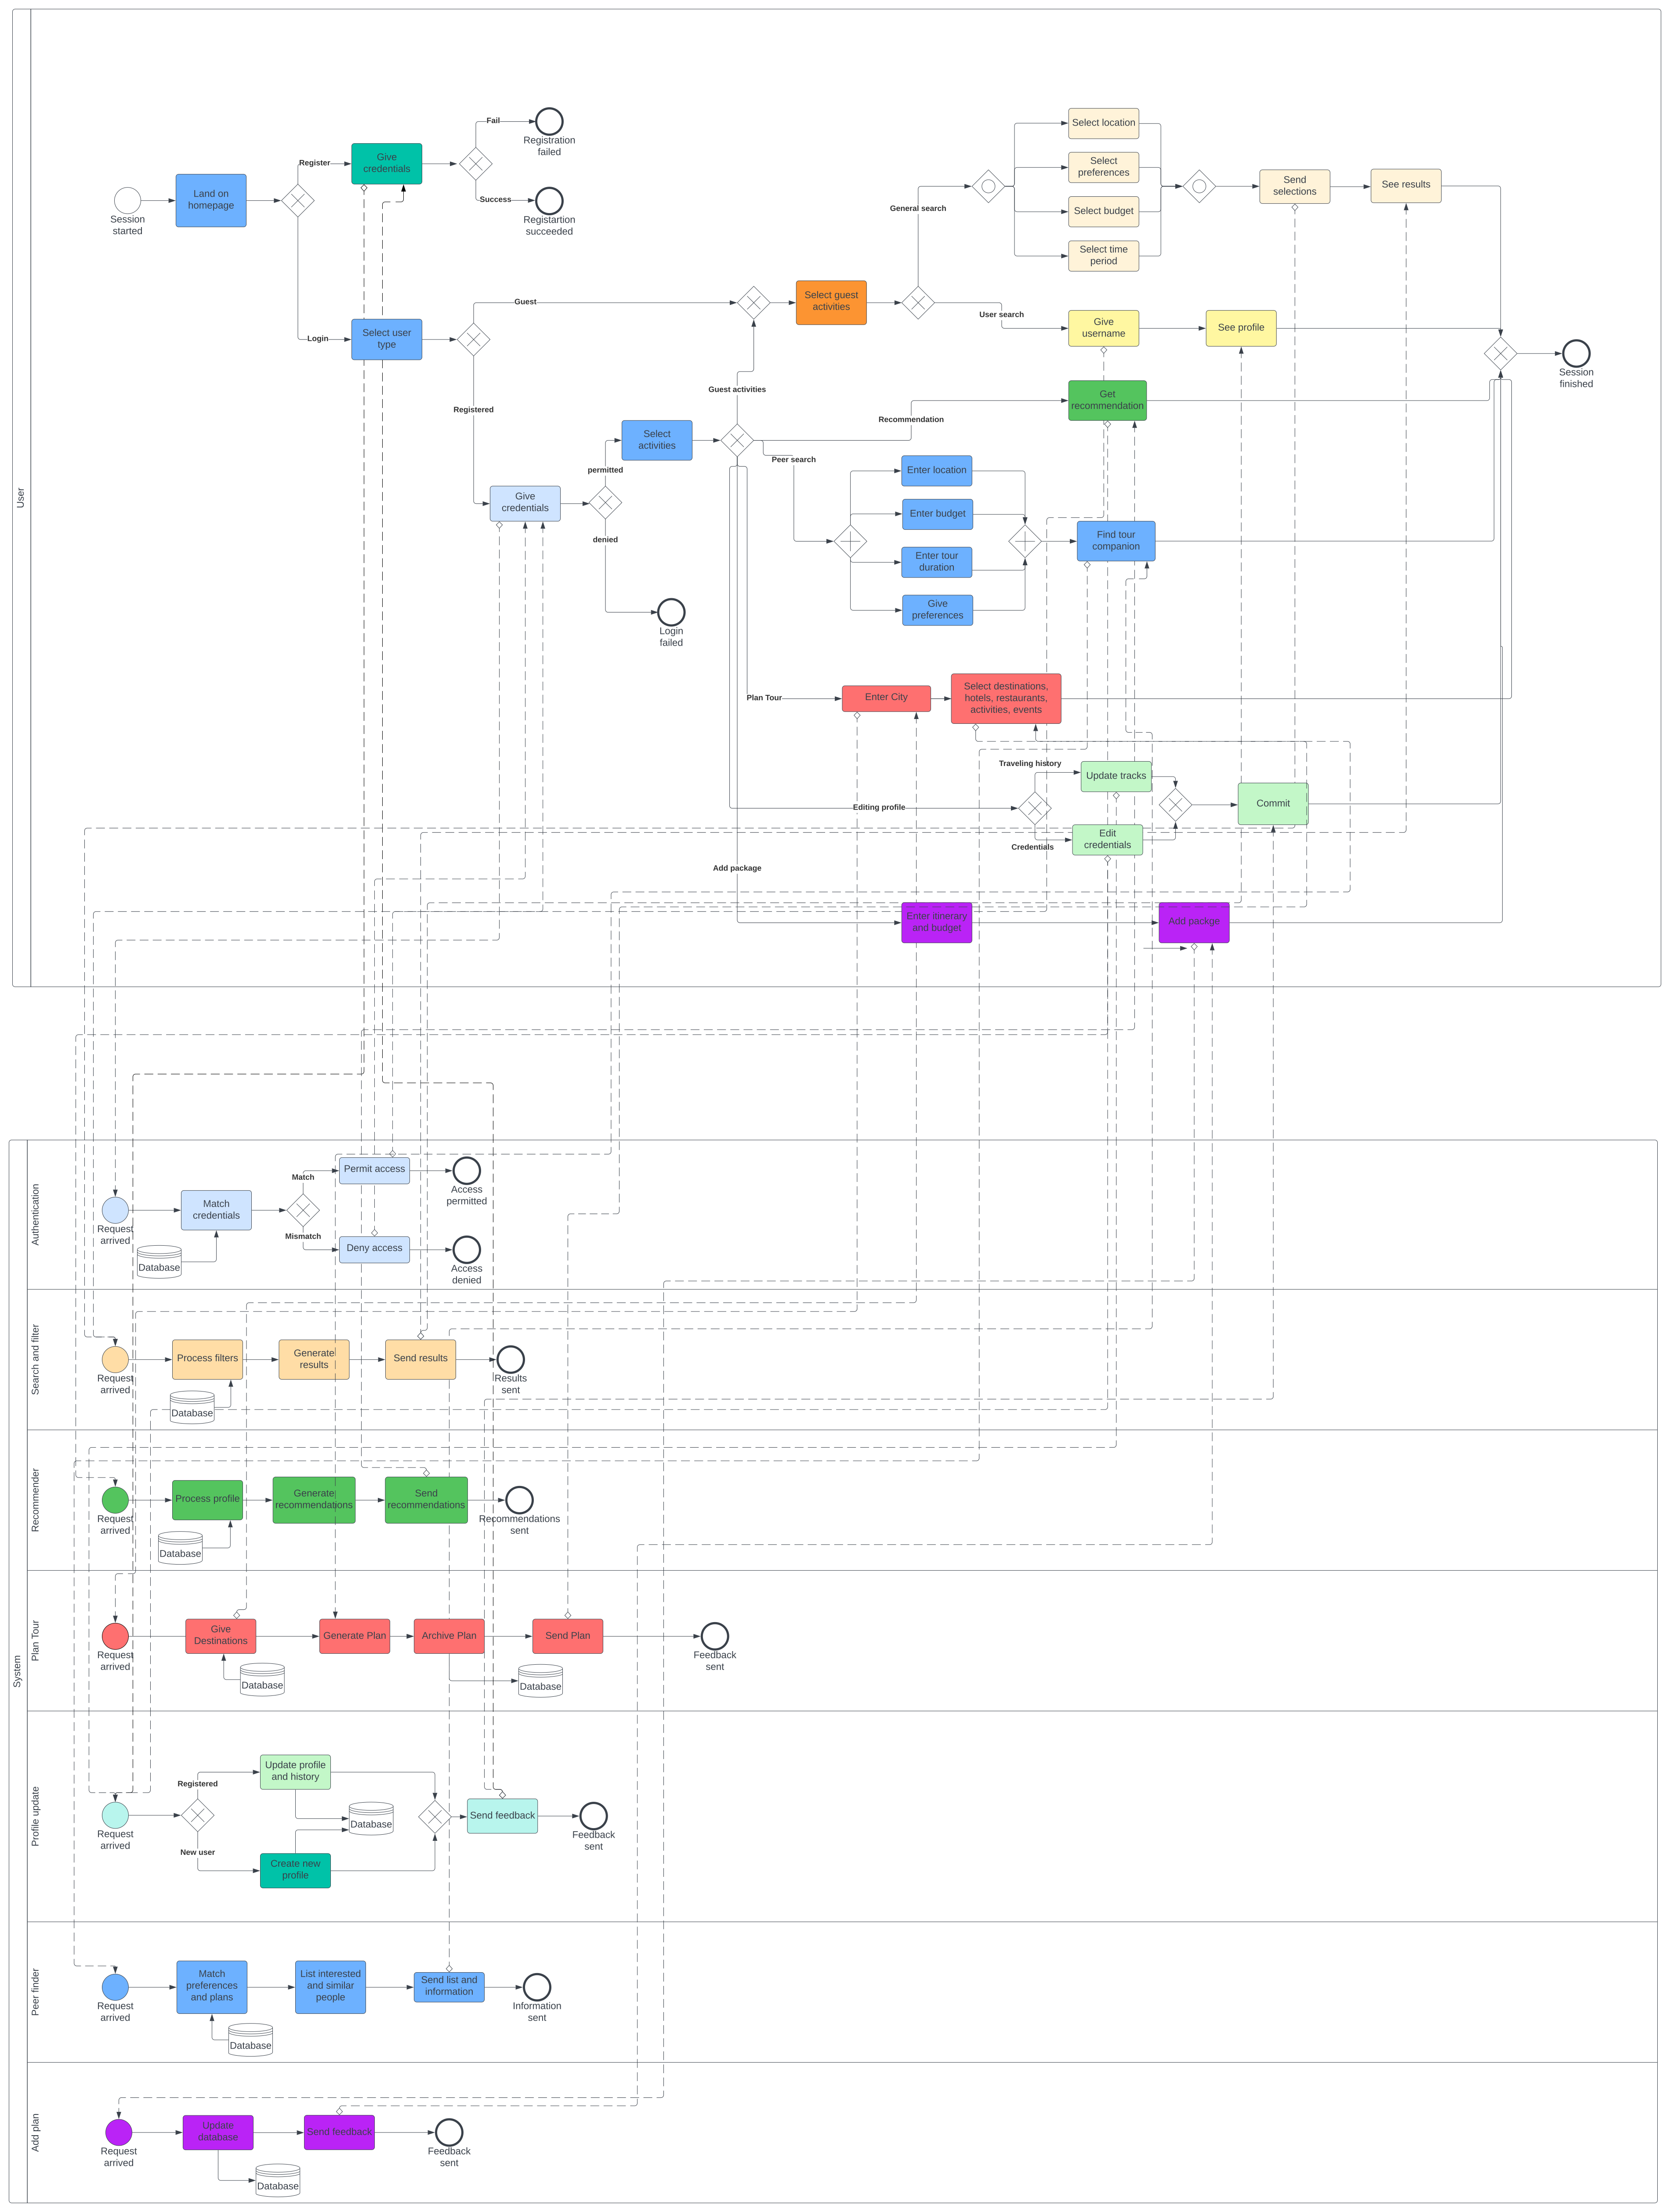
\includegraphics[width=0.80\textwidth]{BPMN/bpmn.png}
        \label{fig:bpmn}
    \caption{The BPMN Diagram}
\end{figure}

\newpage
\subsection{Pools}
\begin{itemize}
    \item User
    \item System
\end{itemize}

\subsubsection{User Pool}
\begin{figure}[H]
    \centering
        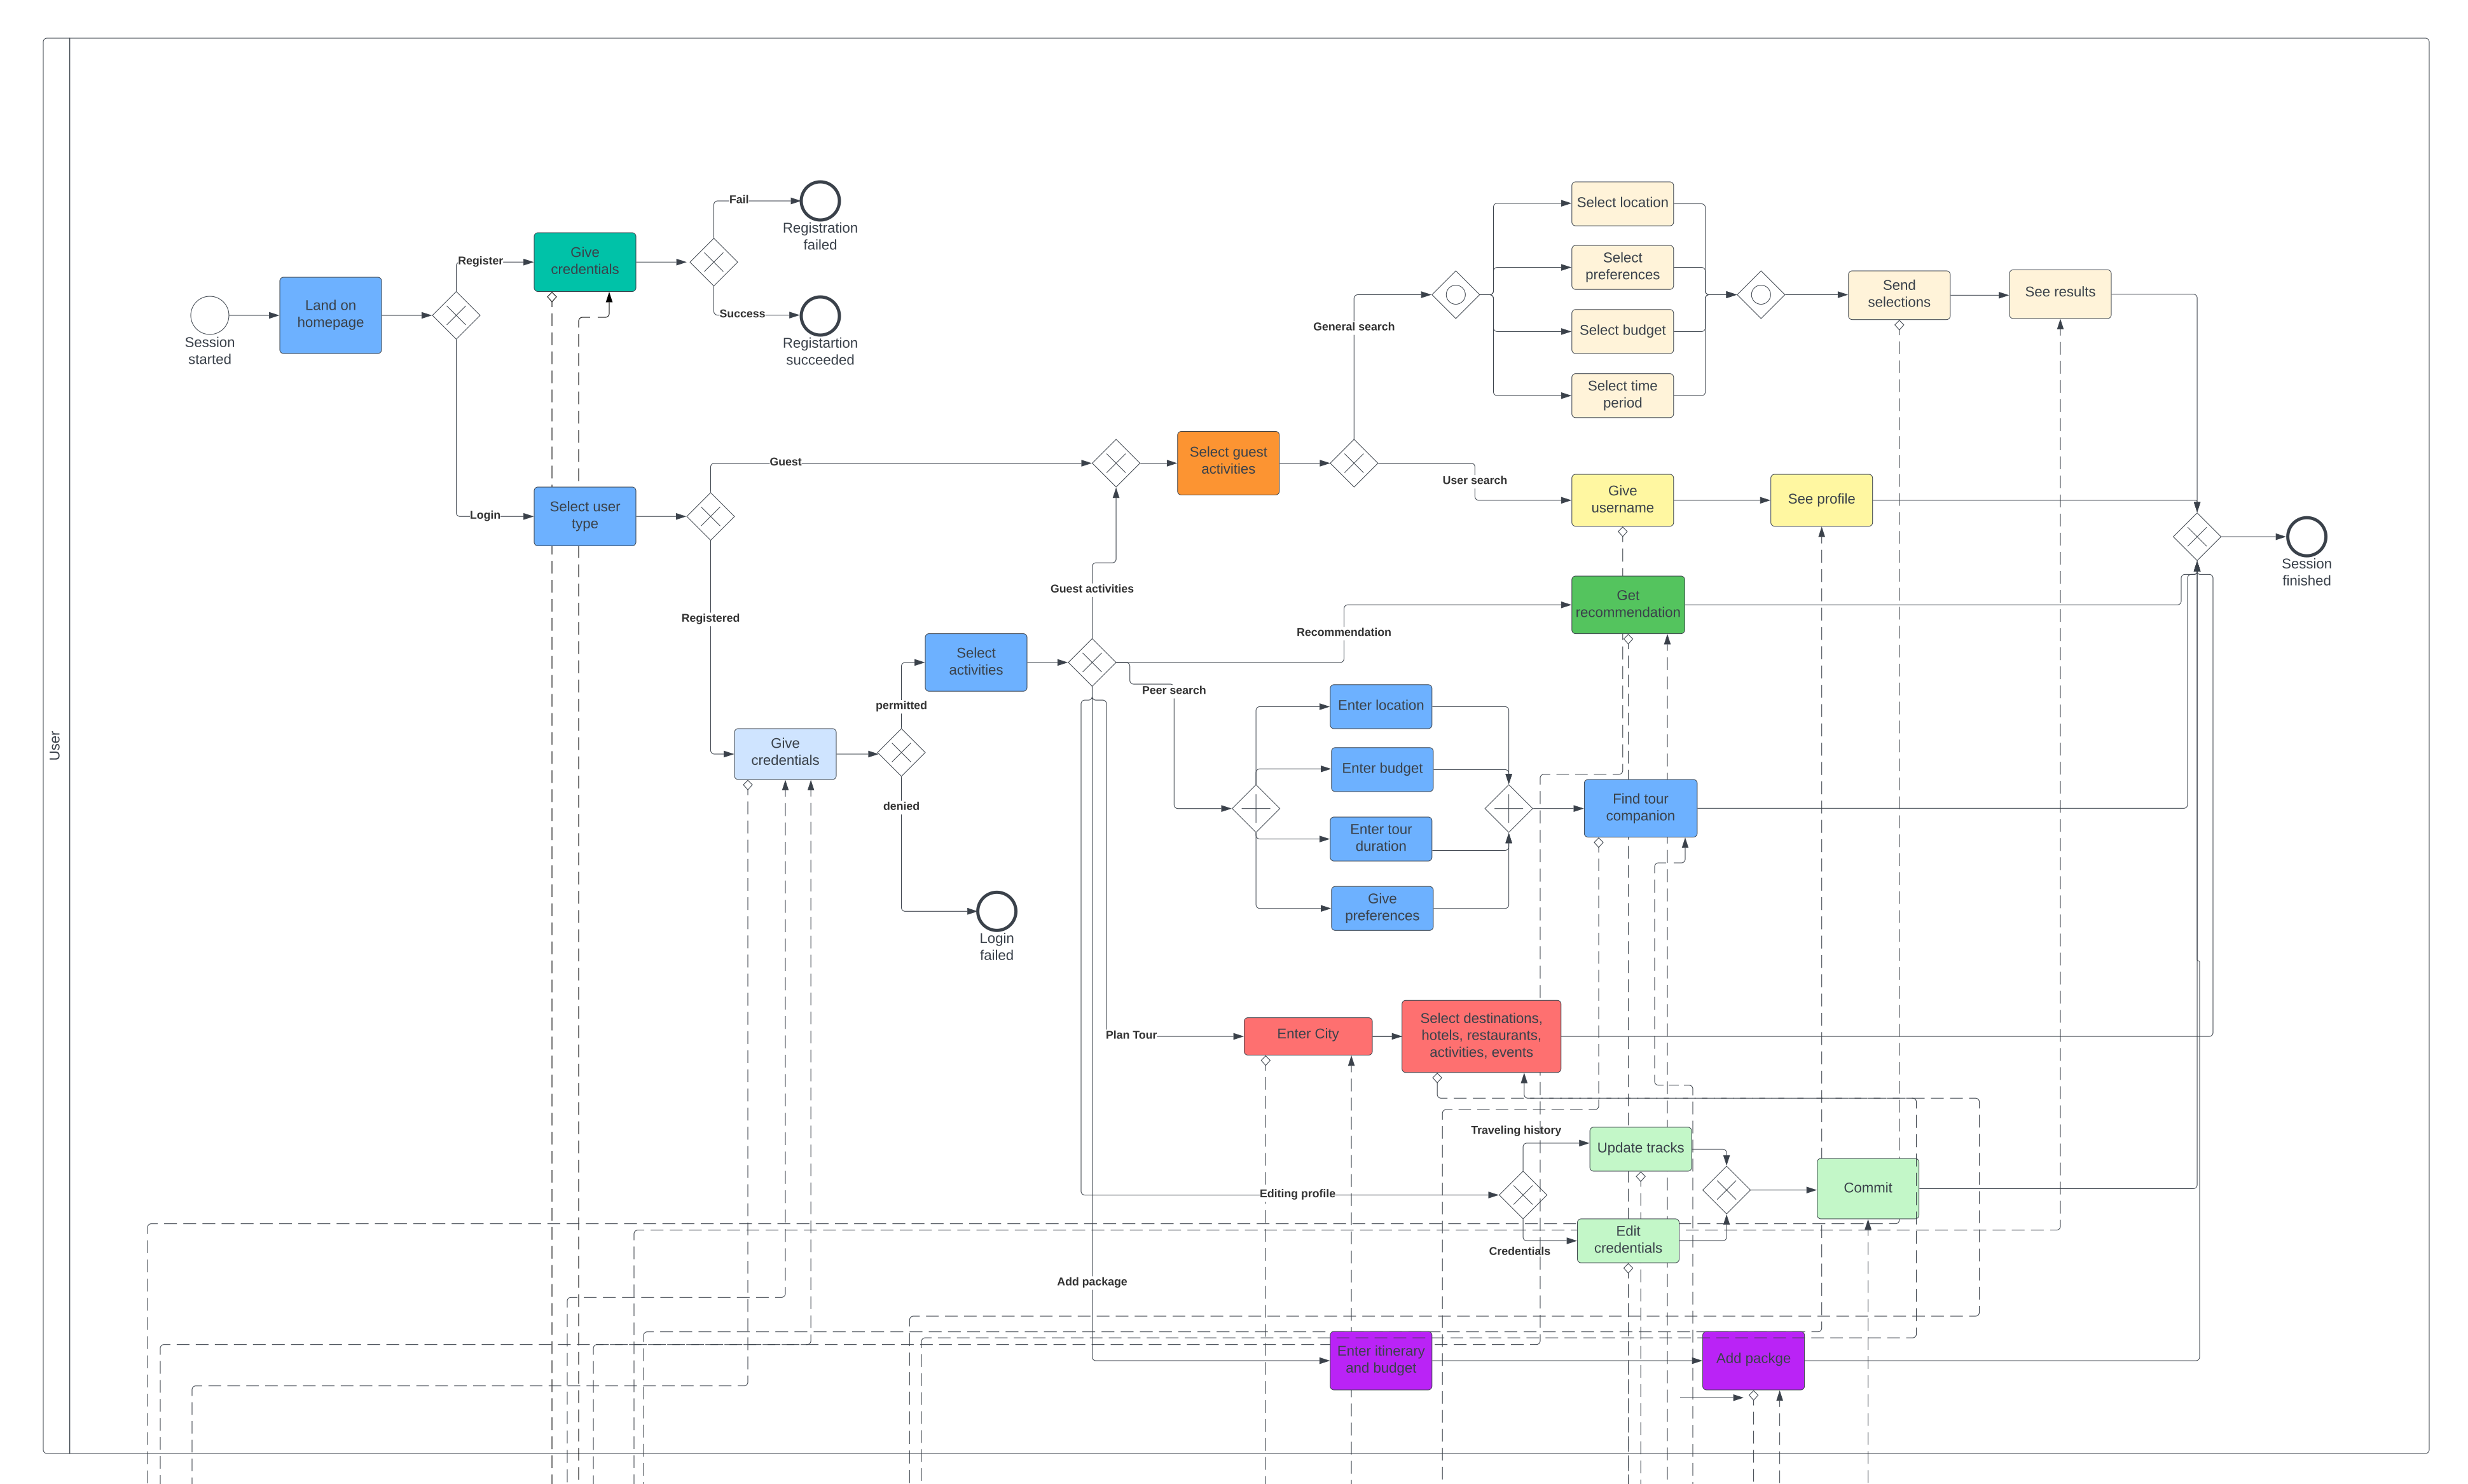
\includegraphics[width=1.0\textwidth]{BPMN/user.png}
        \label{fig:bpmn_userpool}
    \caption{User Pool}
\end{figure}

\newpage
\subsubsection{System Pool}
\begin{figure}[H]
    \centering
        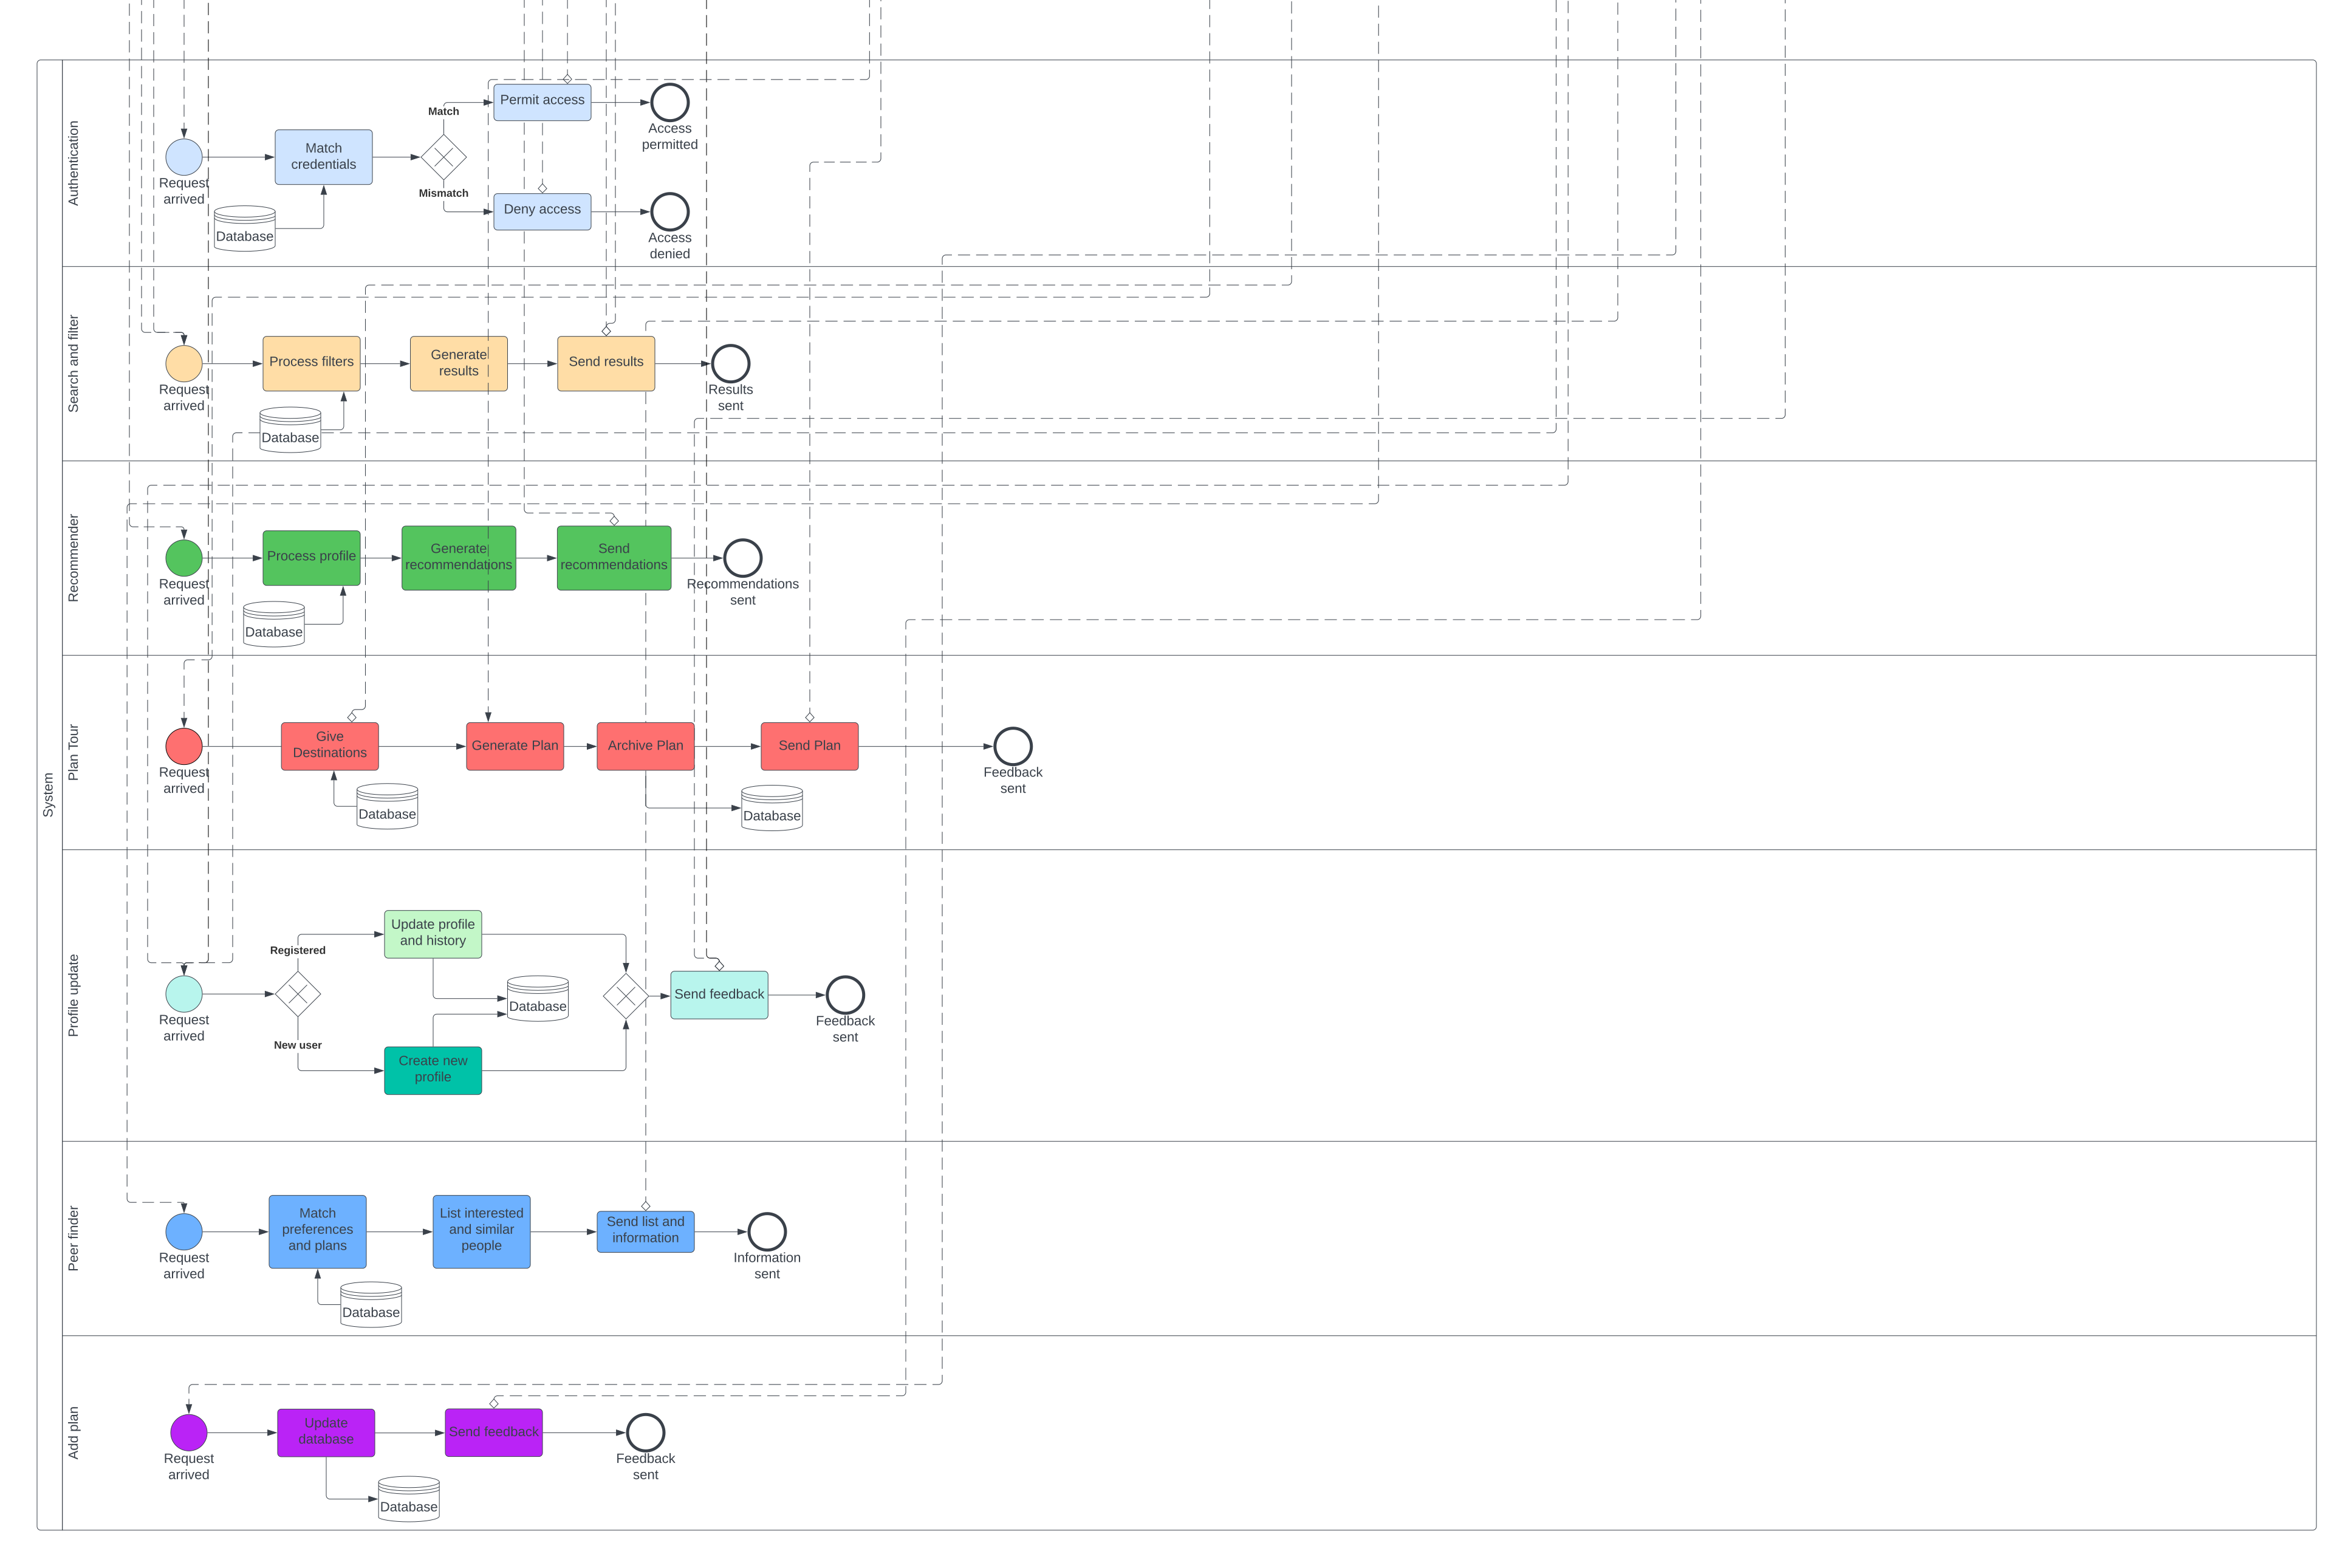
\includegraphics[width=1.0\textwidth]{BPMN/system.png}
        \label{fig:bpmn_systempool}
    \caption{System Pool}
\end{figure}

\newpage

\section{Mock UI}
\subsection{Login Page}
\begin{figure}[H]
    \centering        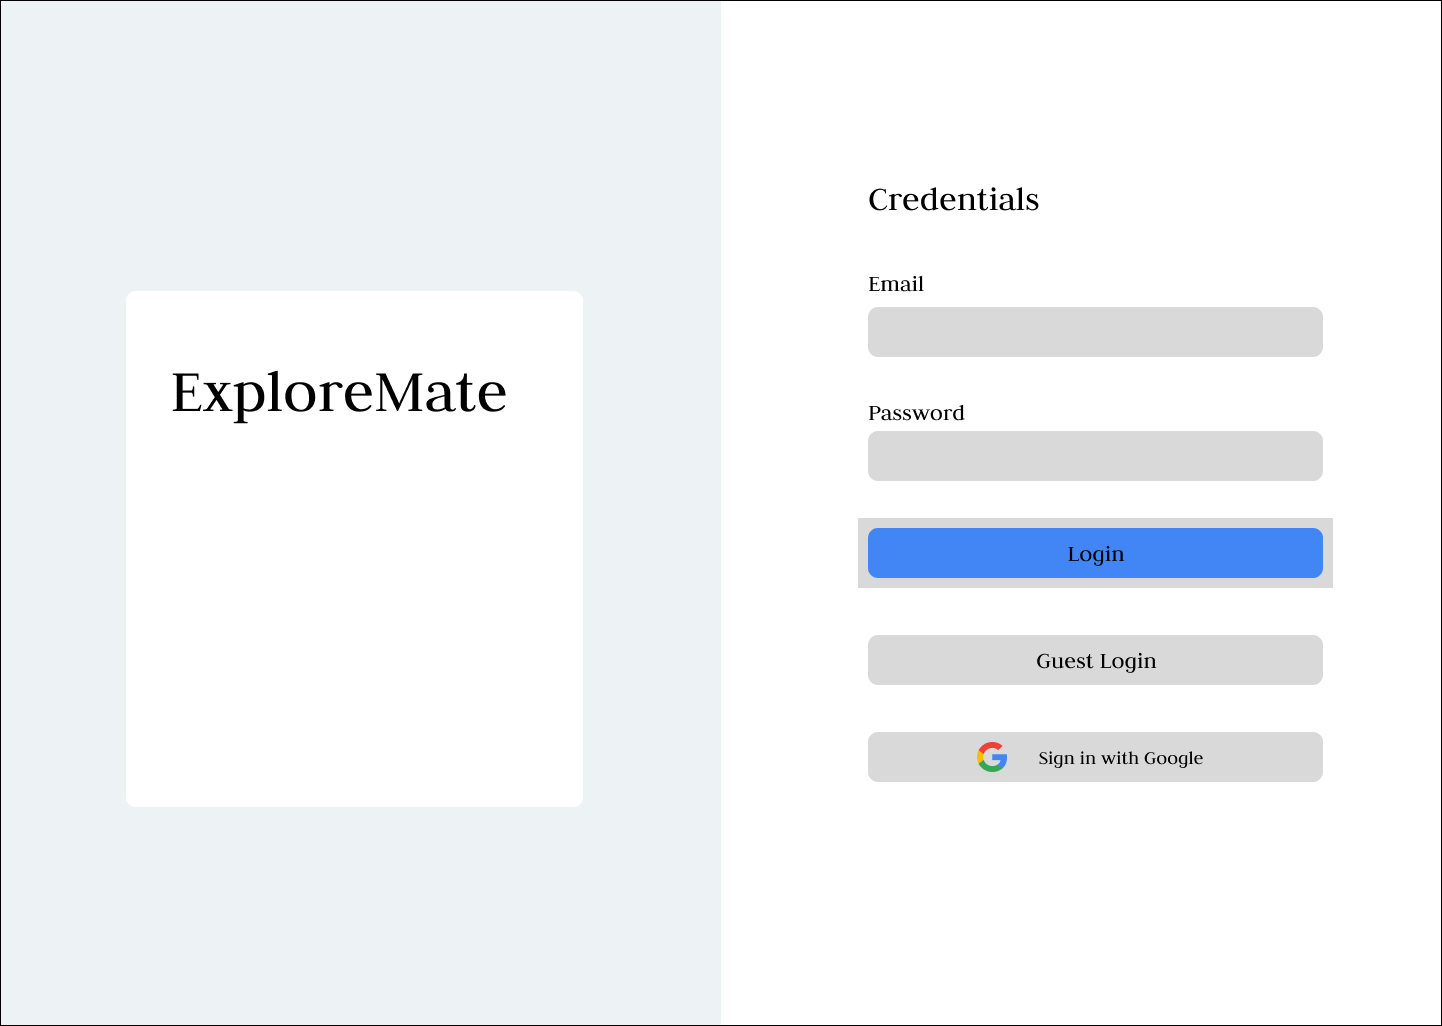
\includegraphics[width=0.9\textwidth]{Mock UI/Login.png}
        \label{fig:login_ui}
    \caption{Login Page}
\end{figure}

\subsection{Home Page}
\begin{figure}[H]
    \centering
        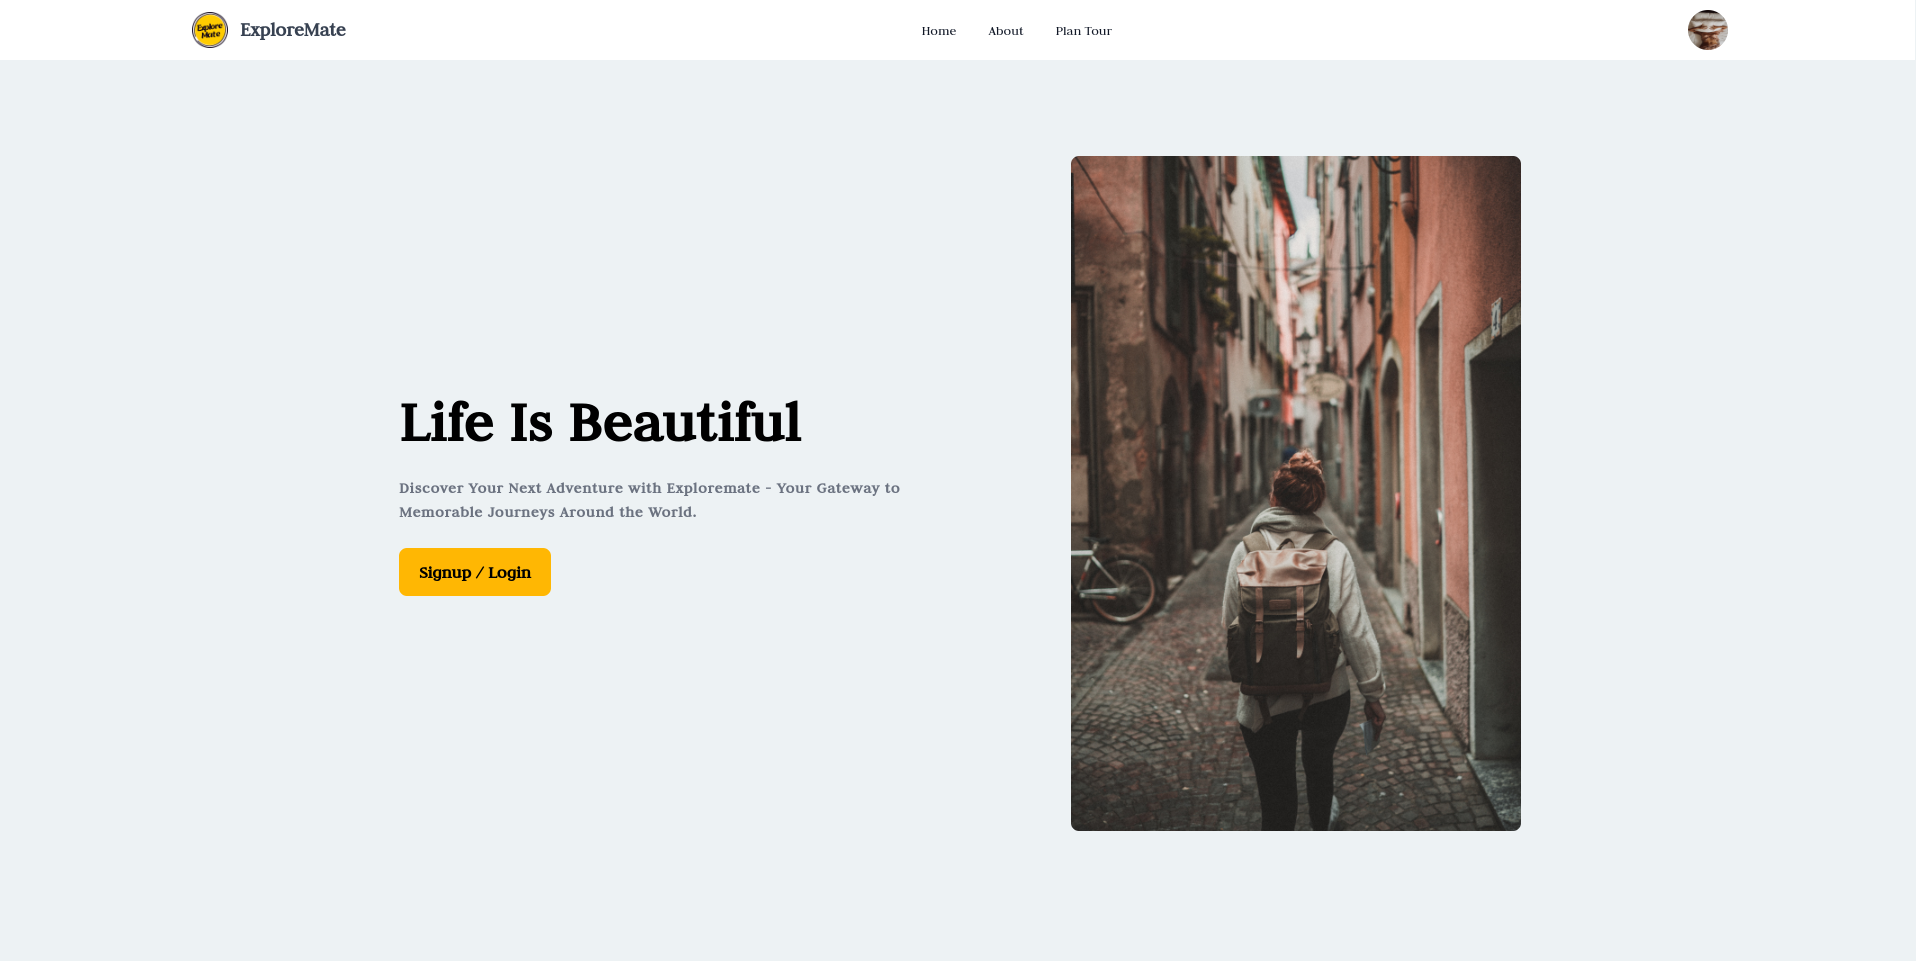
\includegraphics[width=0.9\textwidth]{Mock UI/Home.png}
        \label{fig:home_ui}
    \caption{Home Page}
\end{figure}

\newpage

\subsection{Dashboard}
\begin{figure}[H]
    \centering
        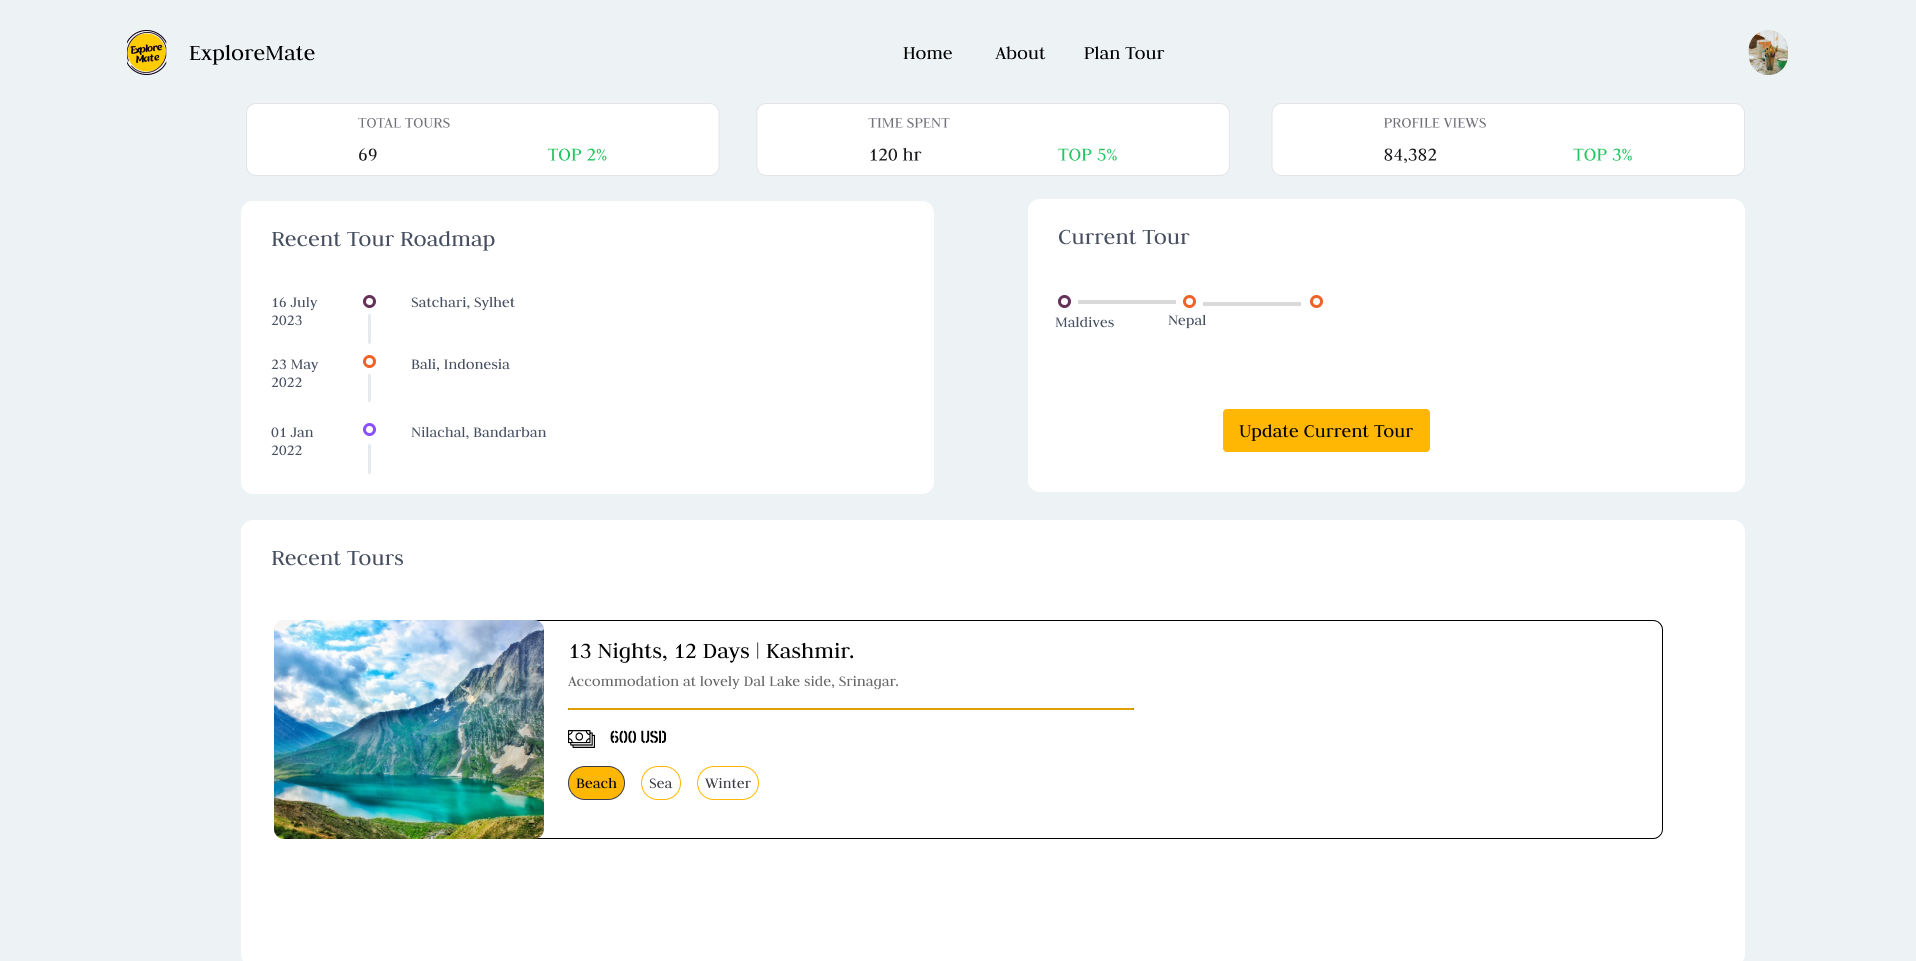
\includegraphics[width=0.9\textwidth]{Mock UI/Dashboard.png}
        \label{fig:dashboard_ui}
    \caption{Dashboard}
\end{figure}

\subsection{Public Profile}
\begin{figure}[H]
    \centering
        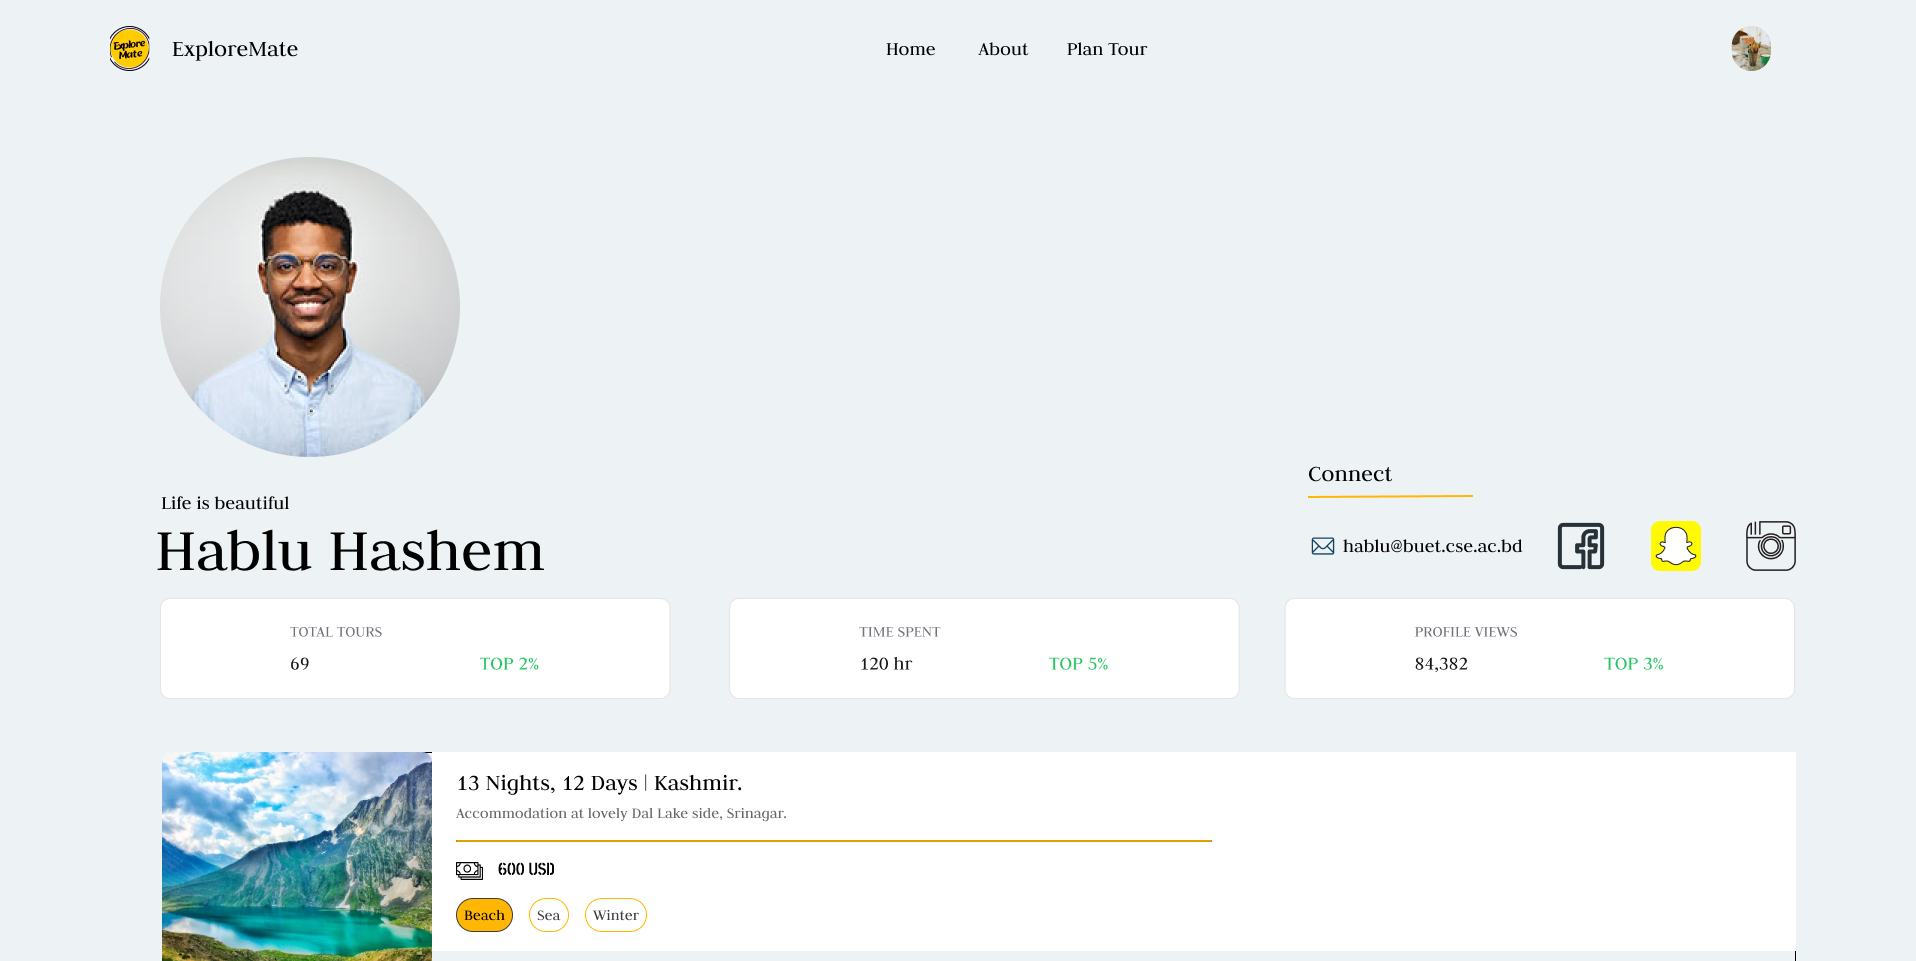
\includegraphics[width=0.9\textwidth]{Mock UI/Public Profile.png}
        \label{fig:public_profile_ui}
    \caption{Public Profile}
\end{figure}

\newpage

\subsection{City Choice Page}
\begin{figure}[H]
    \centering
        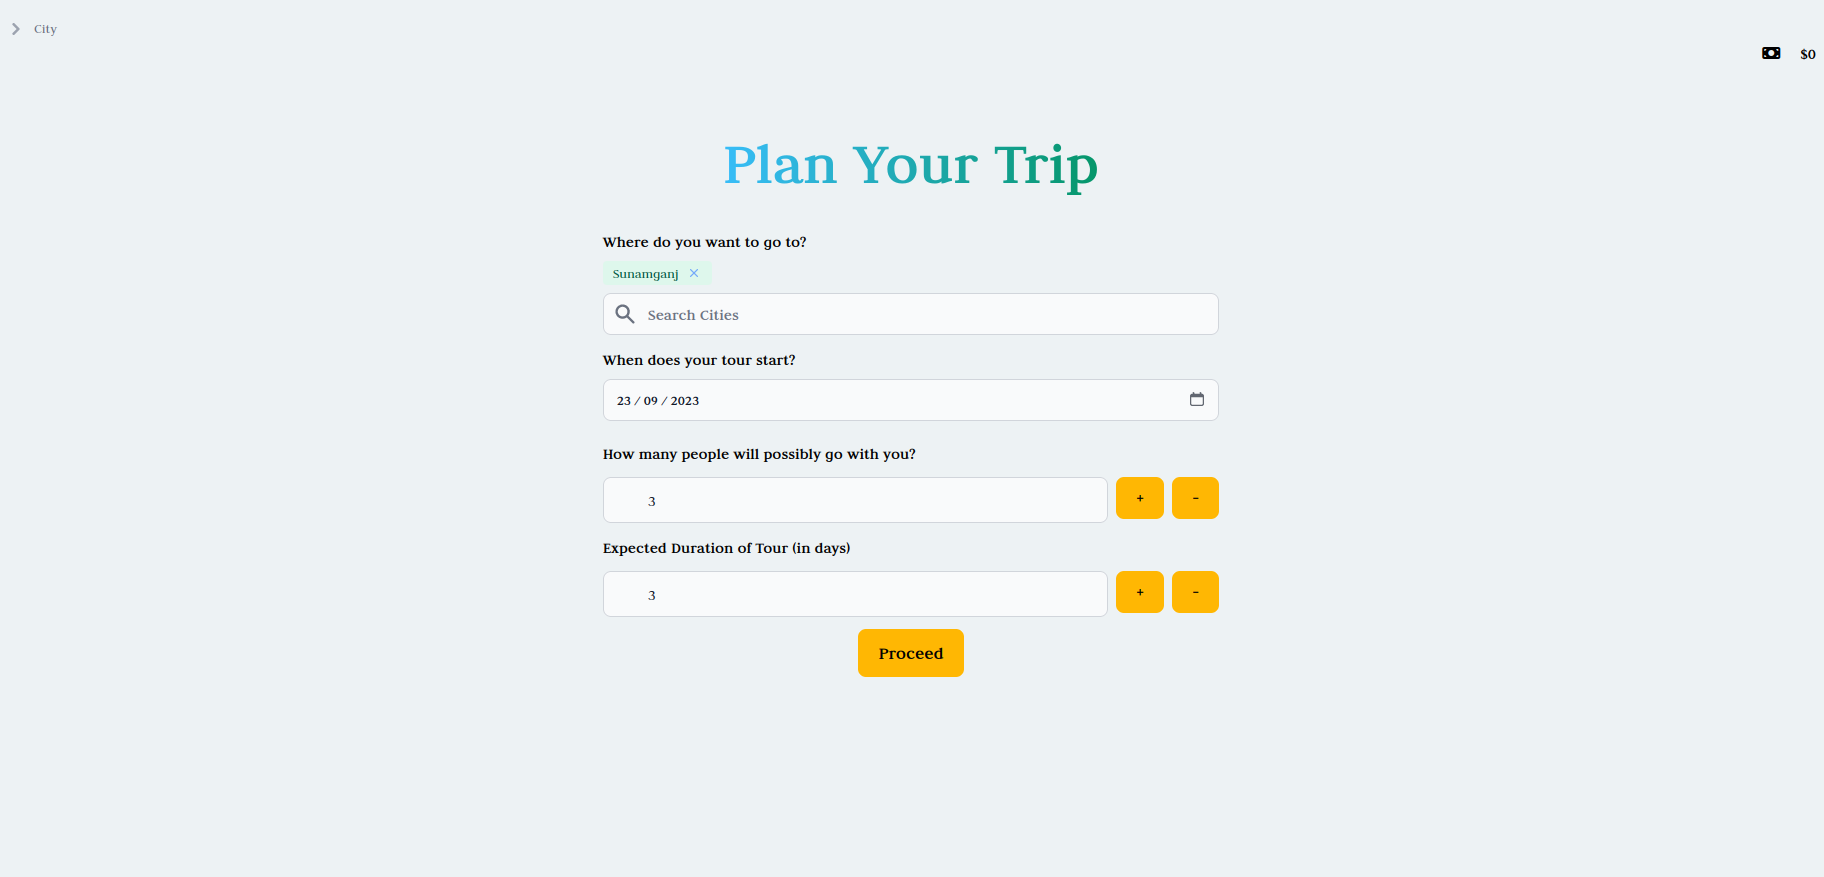
\includegraphics[width=\textwidth]{Mock UI/City Choice.png}
        \label{fig:city_choice_ui}
    \caption{City Choice Page}
\end{figure}

\subsection{Destination Choice}
\begin{figure}[H]
    \centering
        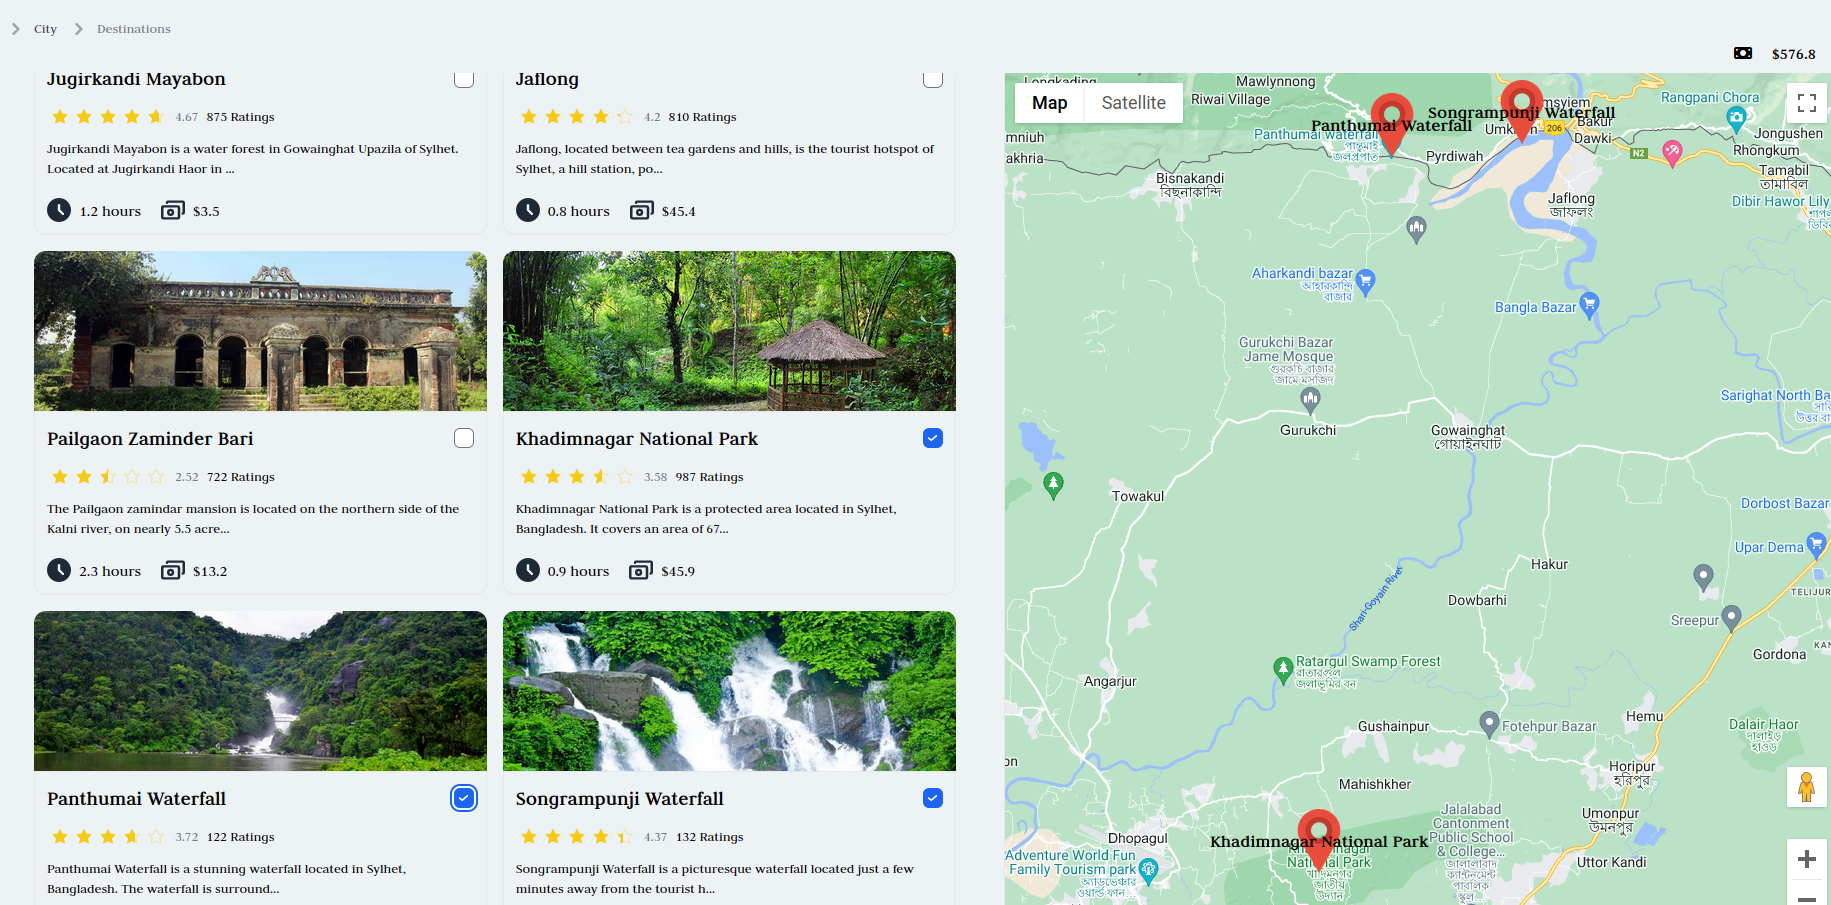
\includegraphics[width=\textwidth]{Mock UI/Destination Choice.png}
        \label{fig:destination_choice_ui}
    \caption{Destination Choice Page}
\end{figure}

\newpage

\subsection{Final Plan}
\begin{figure}[H]
    \centering
        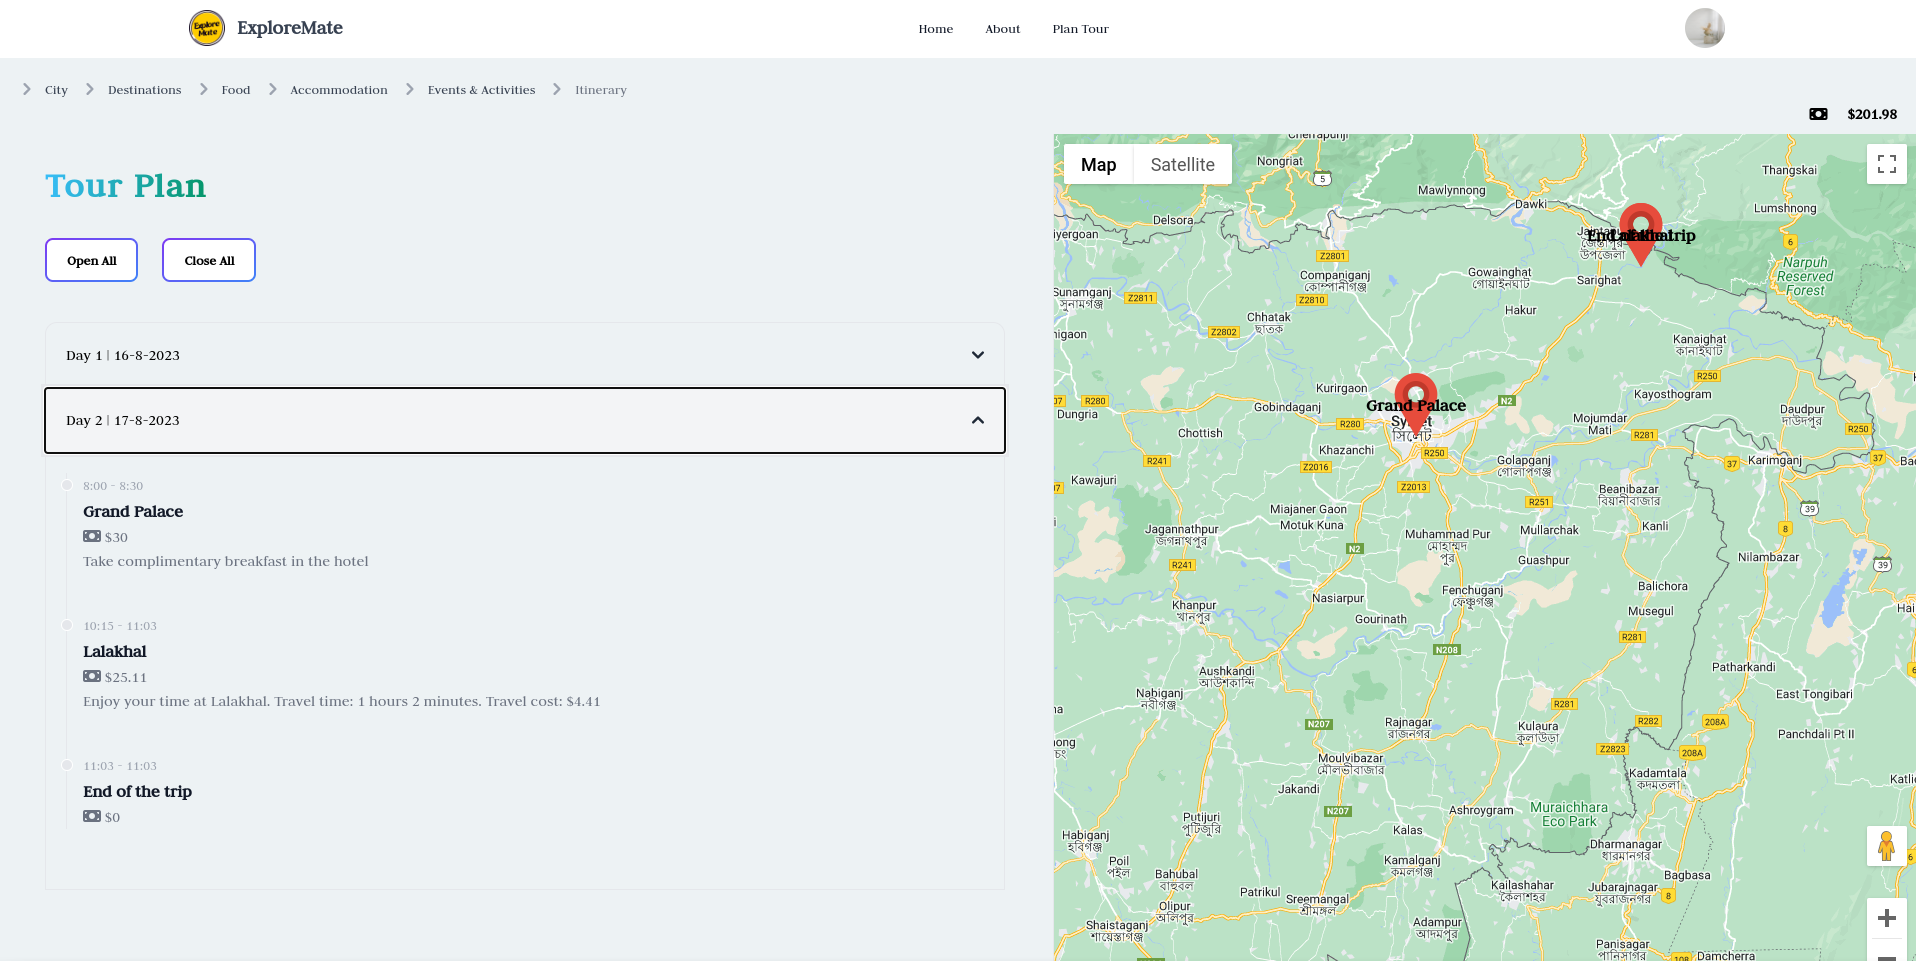
\includegraphics[width=0.9\textwidth]{Mock UI/Final Plan.png}
        \label{fig:final_plan_ui}
    \caption{Final Plan}
\end{figure}

\subsection{Destination Detail}
\begin{figure}[H]
    \centering
        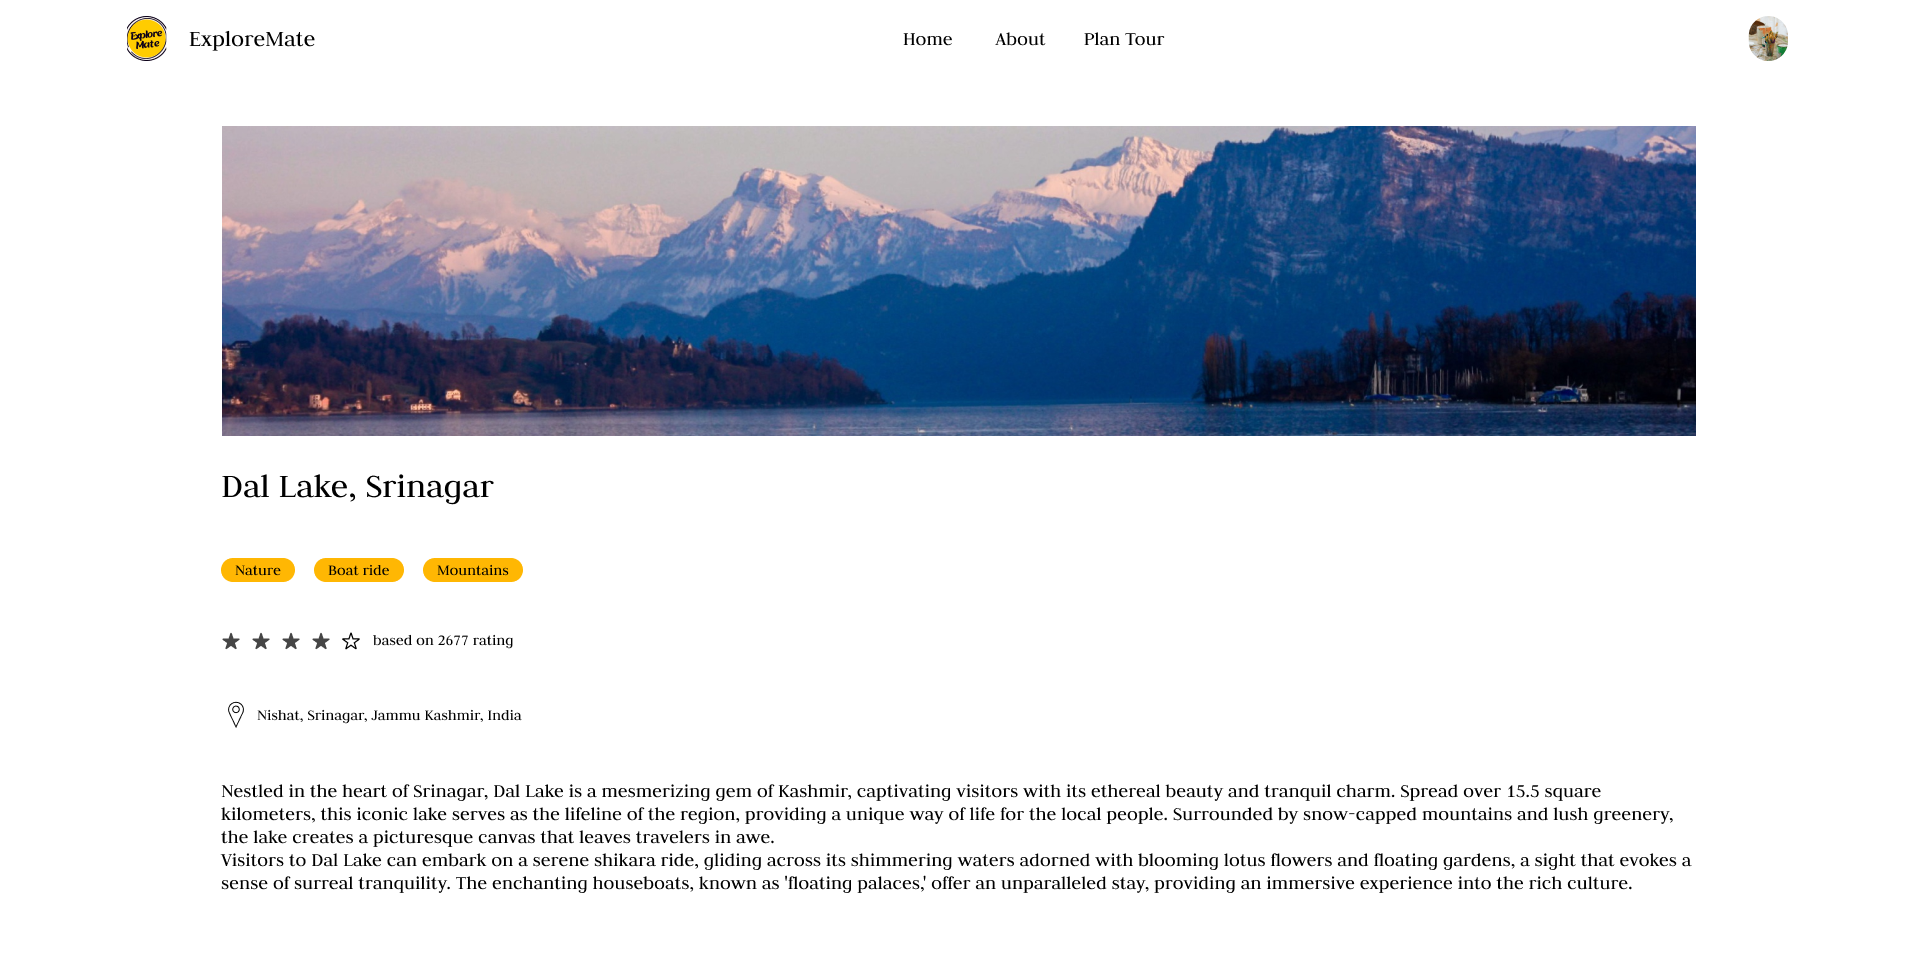
\includegraphics[width=0.9\textwidth]{Mock UI/Destination Detail.png}
        \label{fig:destination_detail_ui}
    \caption{Destination Detail}
\end{figure}

\newpage

\subsection{Tour Detail}
\begin{figure}[H]
    \centering
        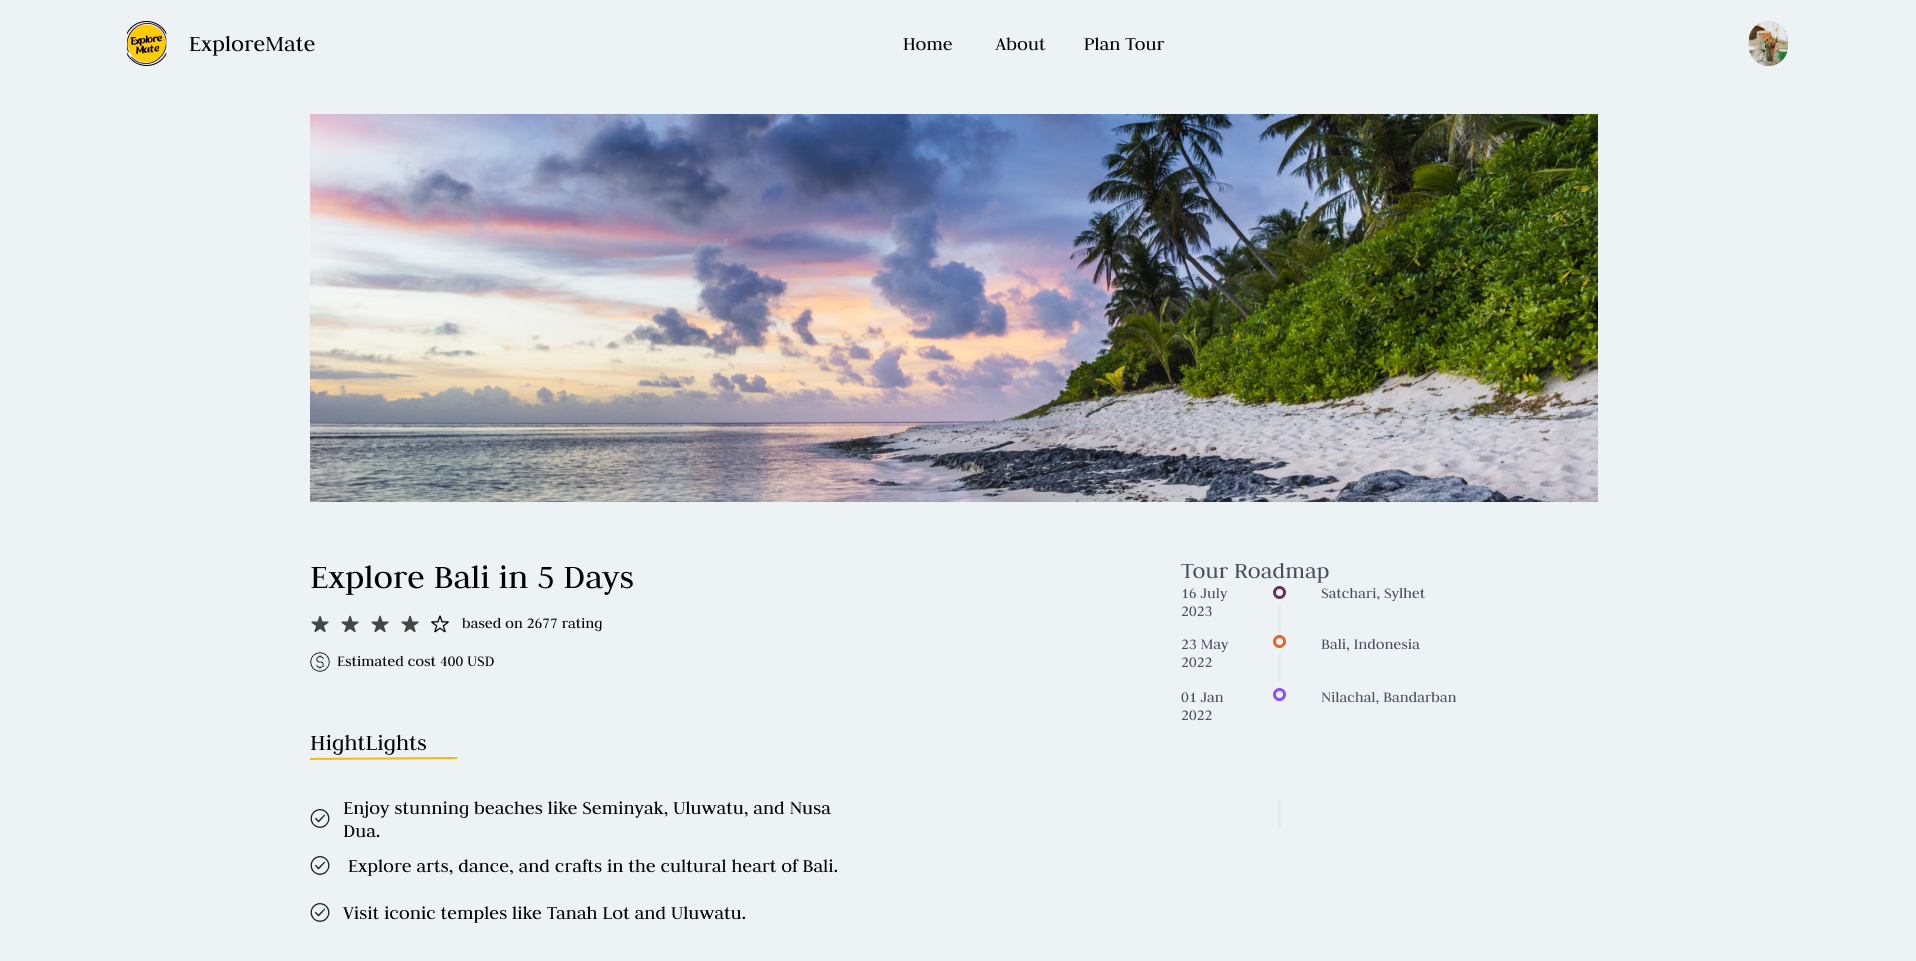
\includegraphics[width=0.9\textwidth]{Mock UI/Tour Detail.png}
        \label{fig:tour_detail_ui}
    \caption{Tour Detail}
\end{figure}

\subsection{Travel Buddy}
\begin{figure}[H]
    \centering
        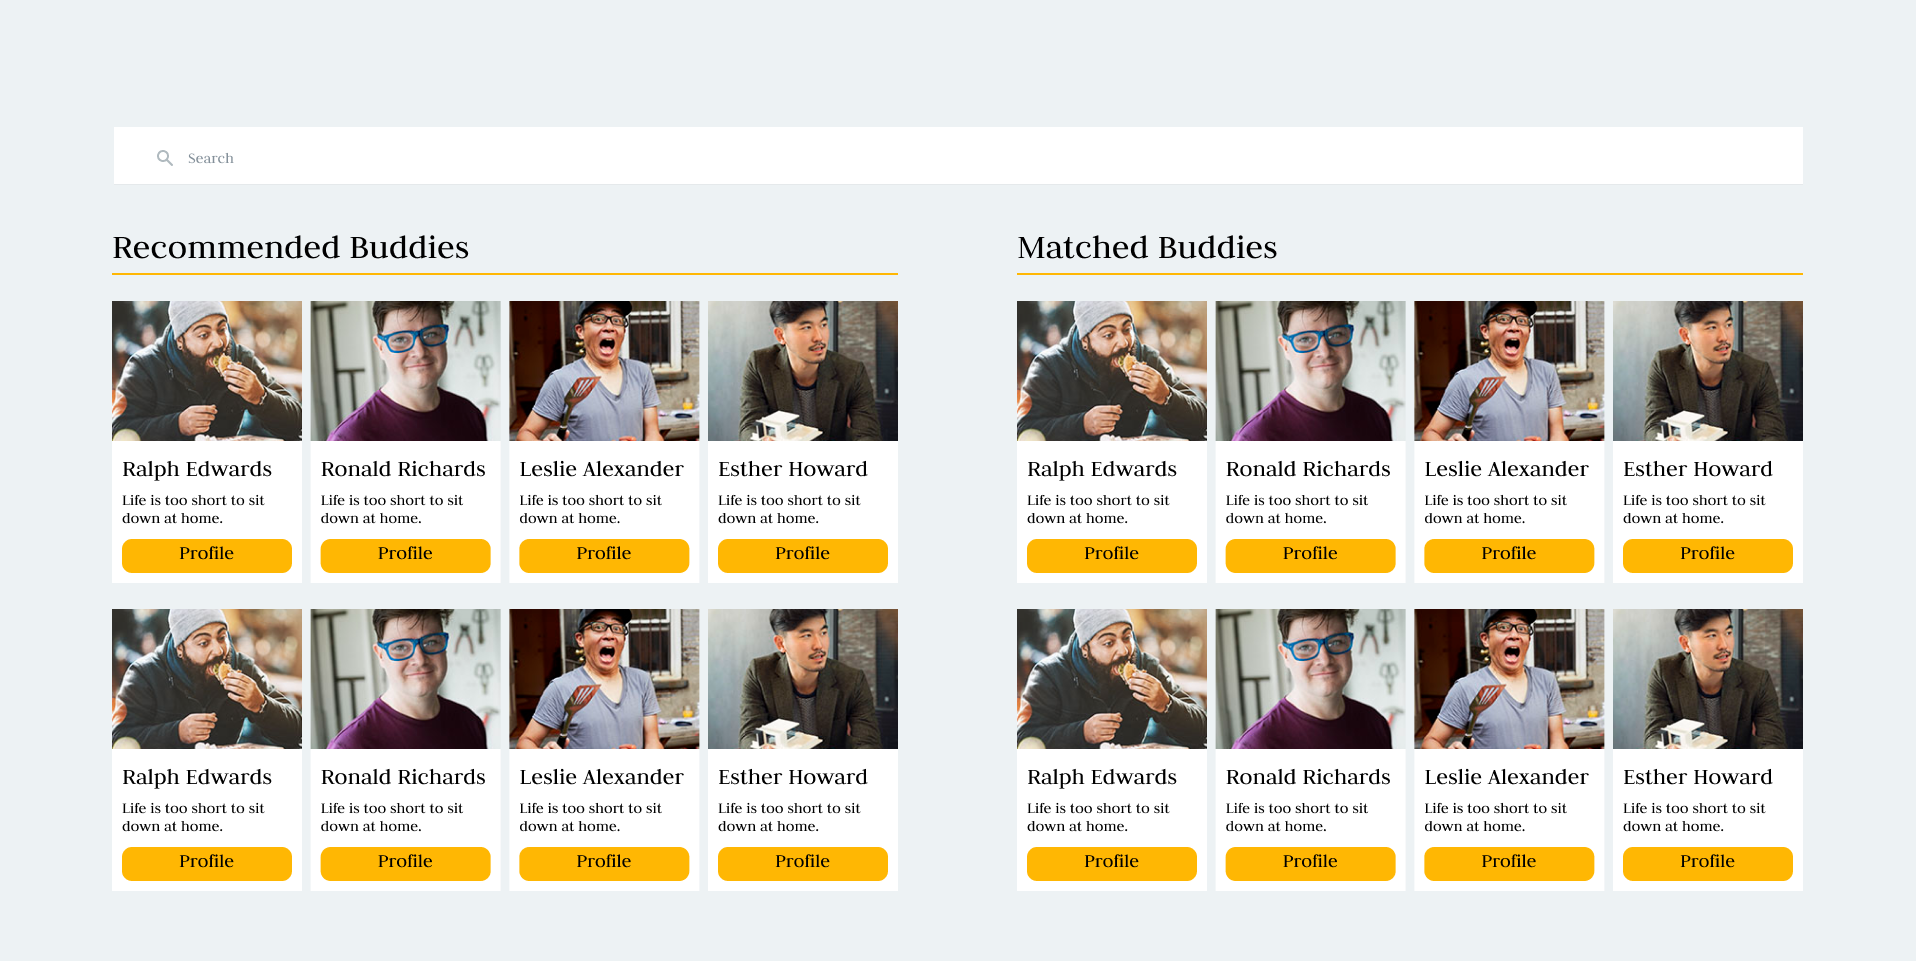
\includegraphics[width=0.9\textwidth]{Mock UI/Travel Buddy.png}
        \label{fig:travel_buddy_ui}
    \caption{Travel Buddy}
\end{figure}

\newpage

\section{ERD}
\subsection{Feedbacks Acknowledged}

\begin{itemize}
    \item Attribute for transportation cost added
\end{itemize}

\subsection{Full ERD}
\begin{figure}[H]
    \centering
        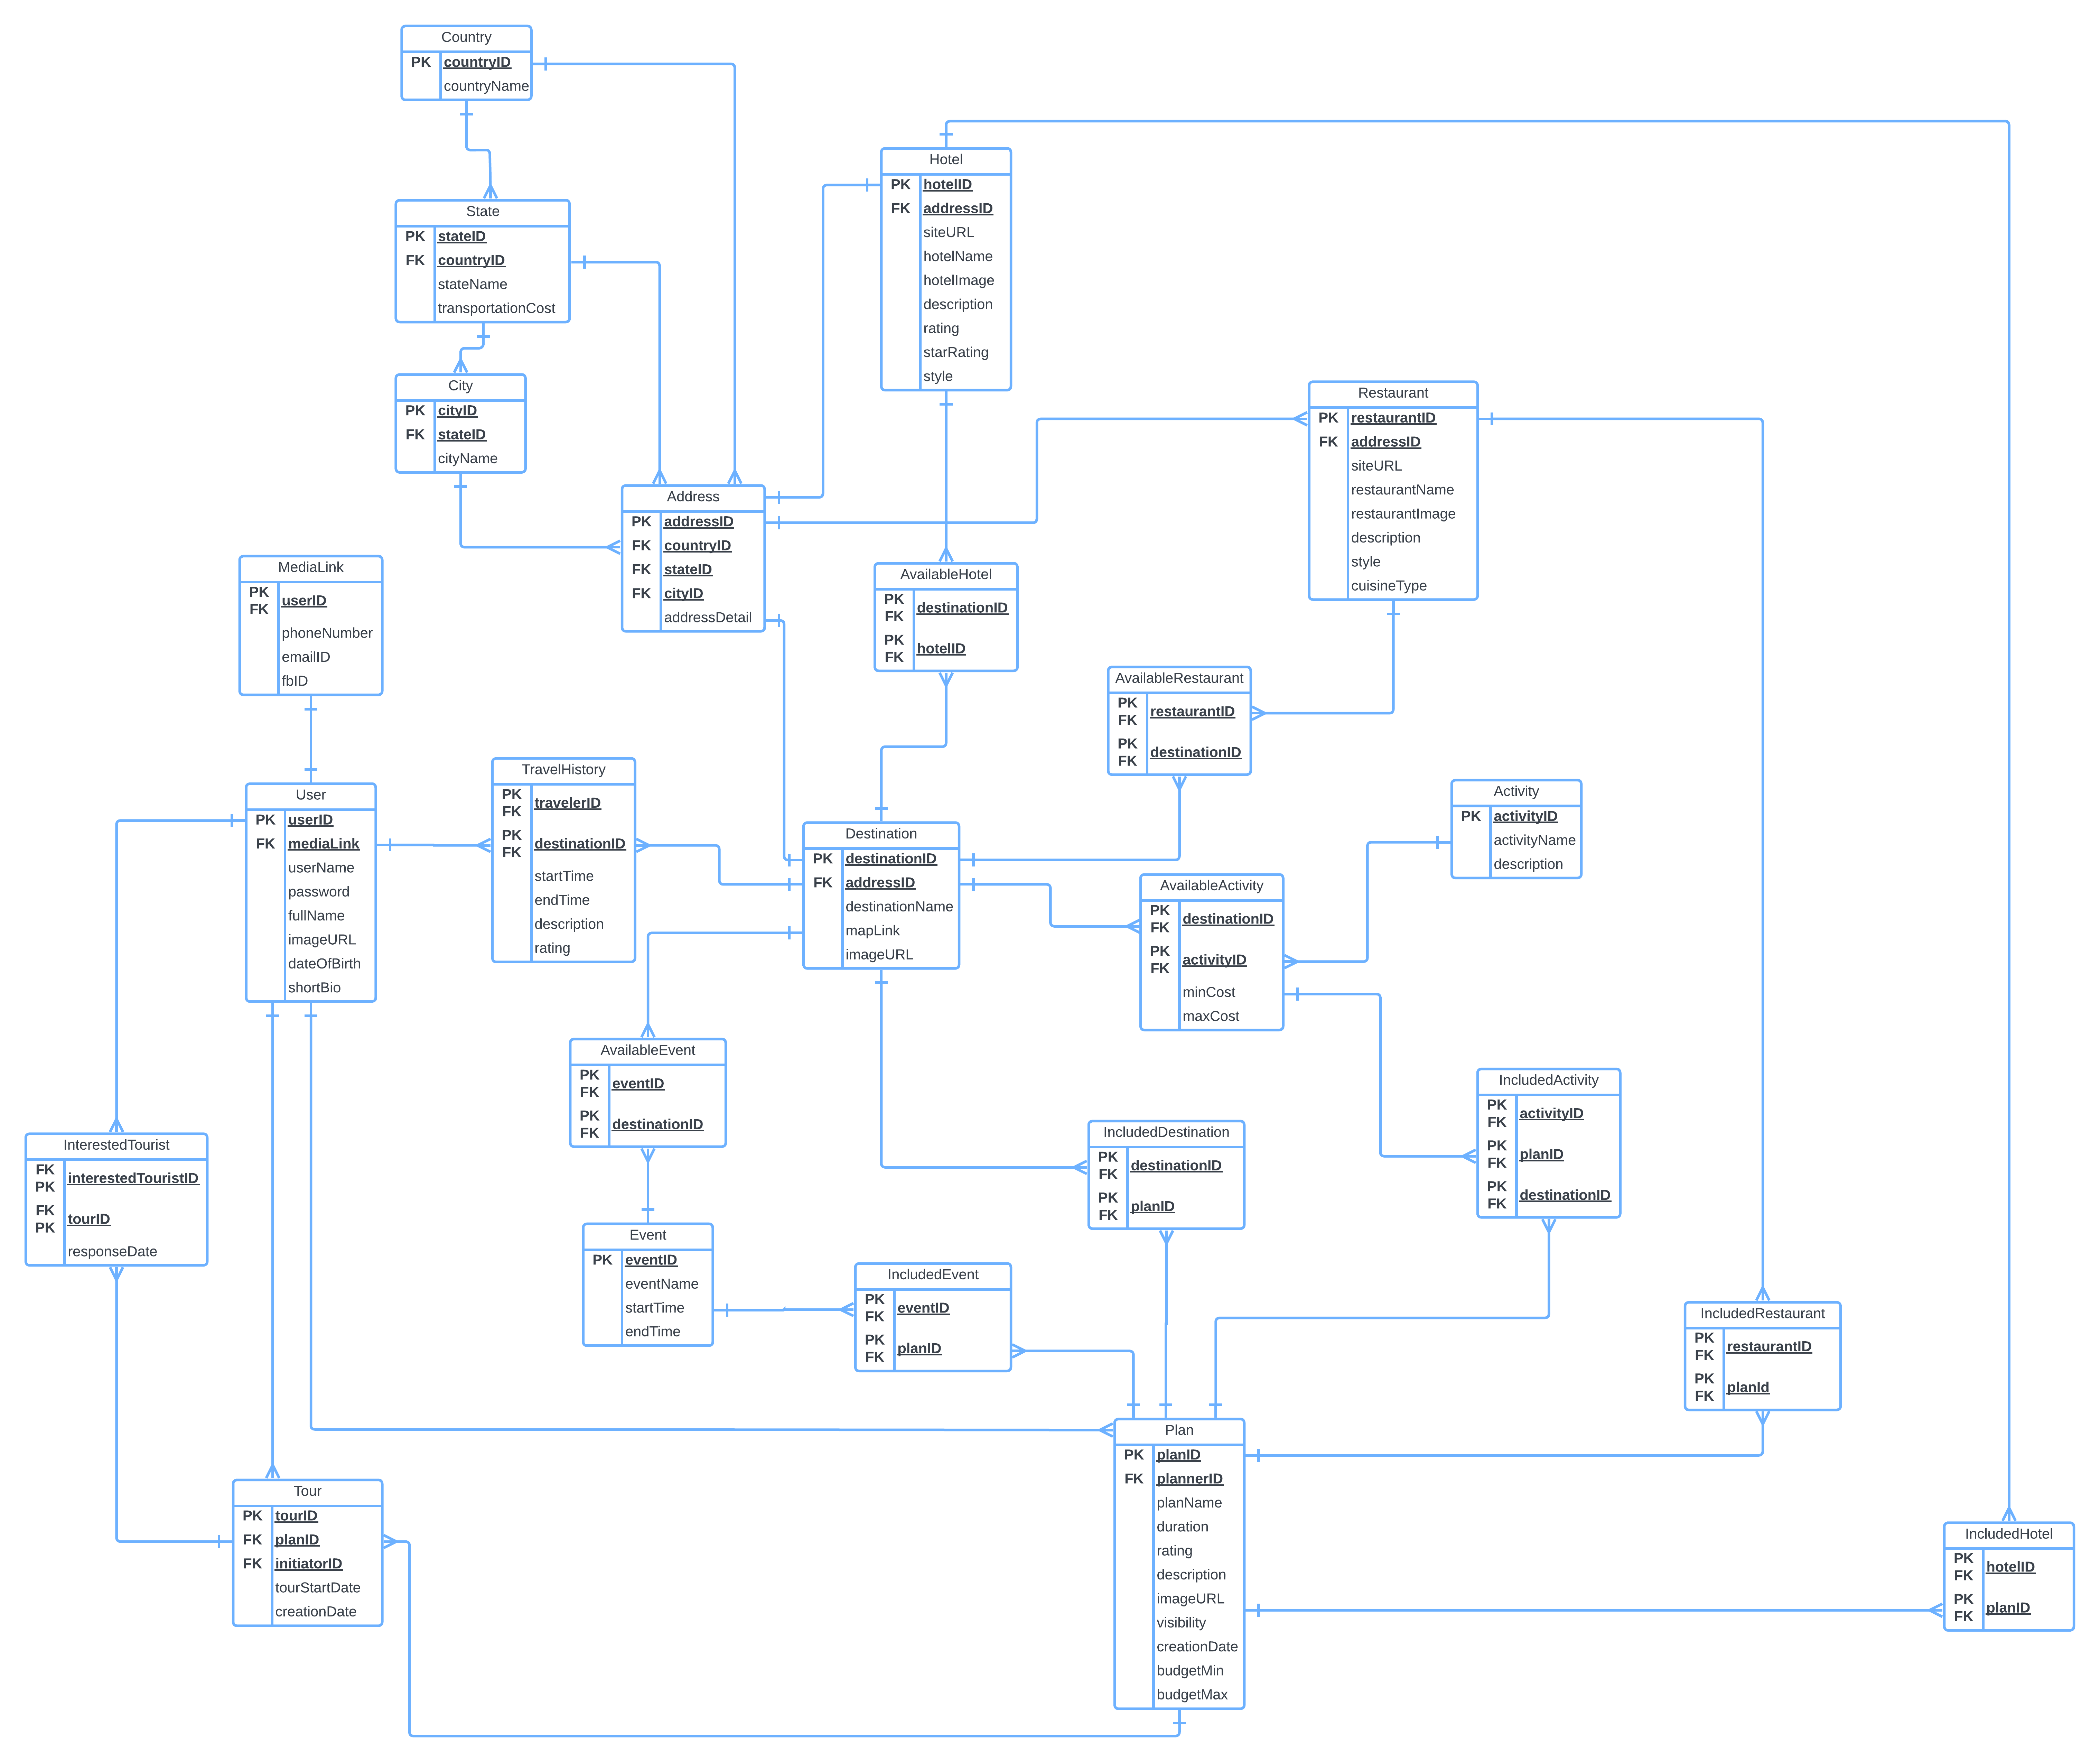
\includegraphics[width=0.85\textwidth]{ERD.png}
        \label{fig:ERD}
    \caption{ERD}
\end{figure}

\newpage

\section{Class Diagrams}
\subsection{Feedbacks Acknowledged}

\begin{itemize}
    \item Country, State and City entity classes are added
    \item Attribute for transportation cost added
\end{itemize}

\subsection{User Authentication}
\begin{figure}[H]
    \centering
        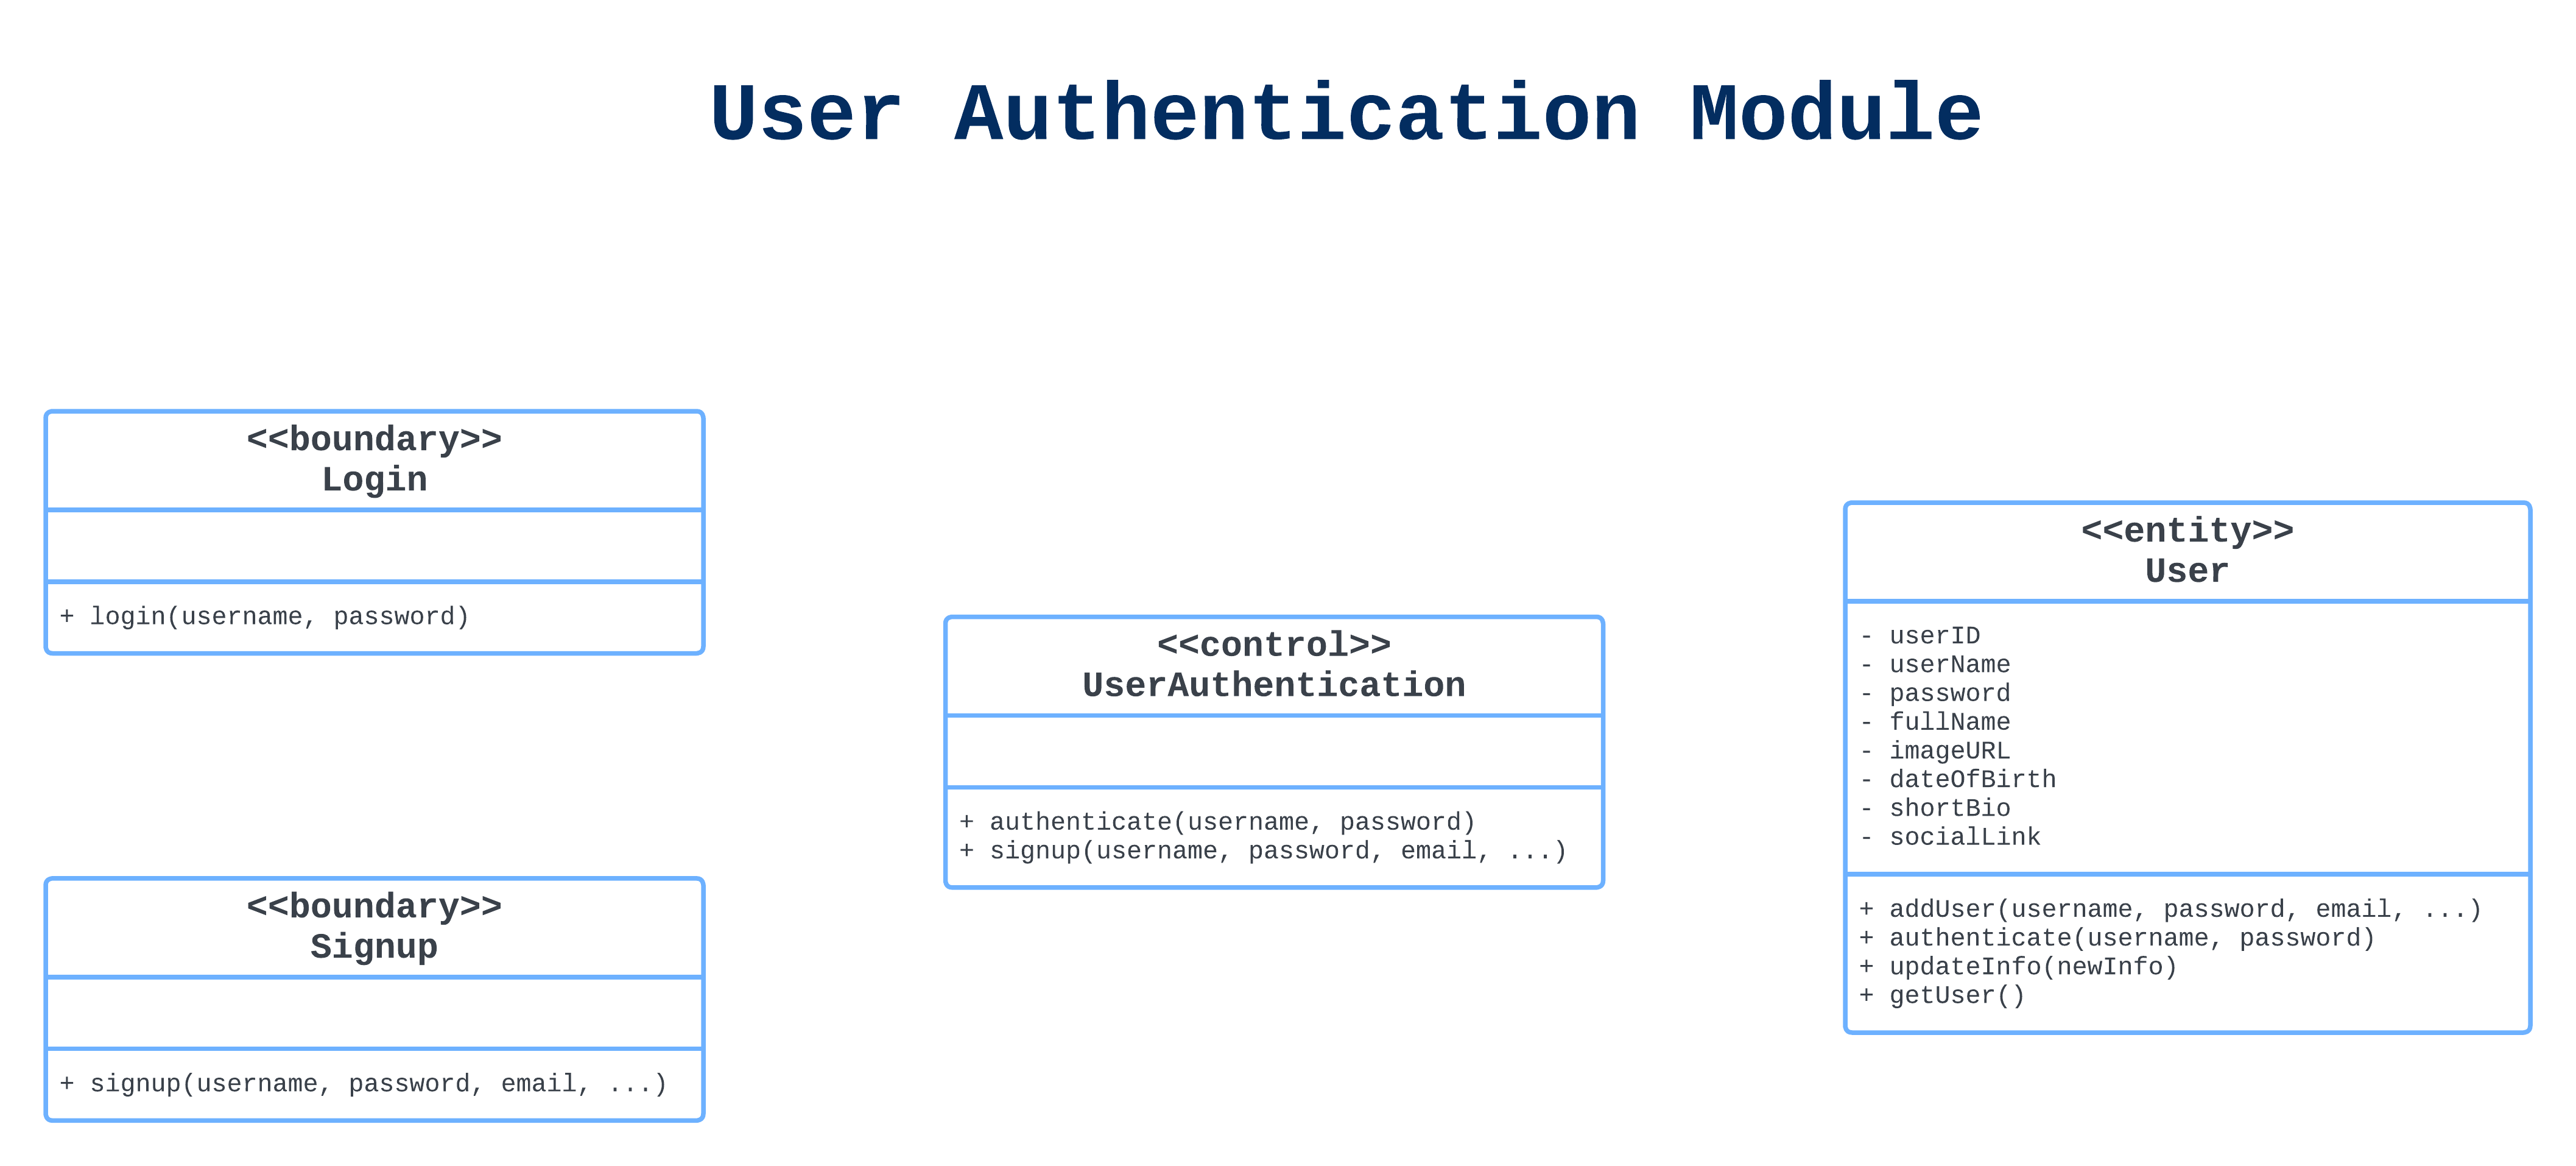
\includegraphics[width=0.85\textwidth]{Class Diagram/User Authentication.png}
        \label{fig:ClassAuth}
    \caption{Class Diagram - User Authentication}
\end{figure}

\subsection{Profile Dashboard}
\begin{figure}[H]
    \centering
        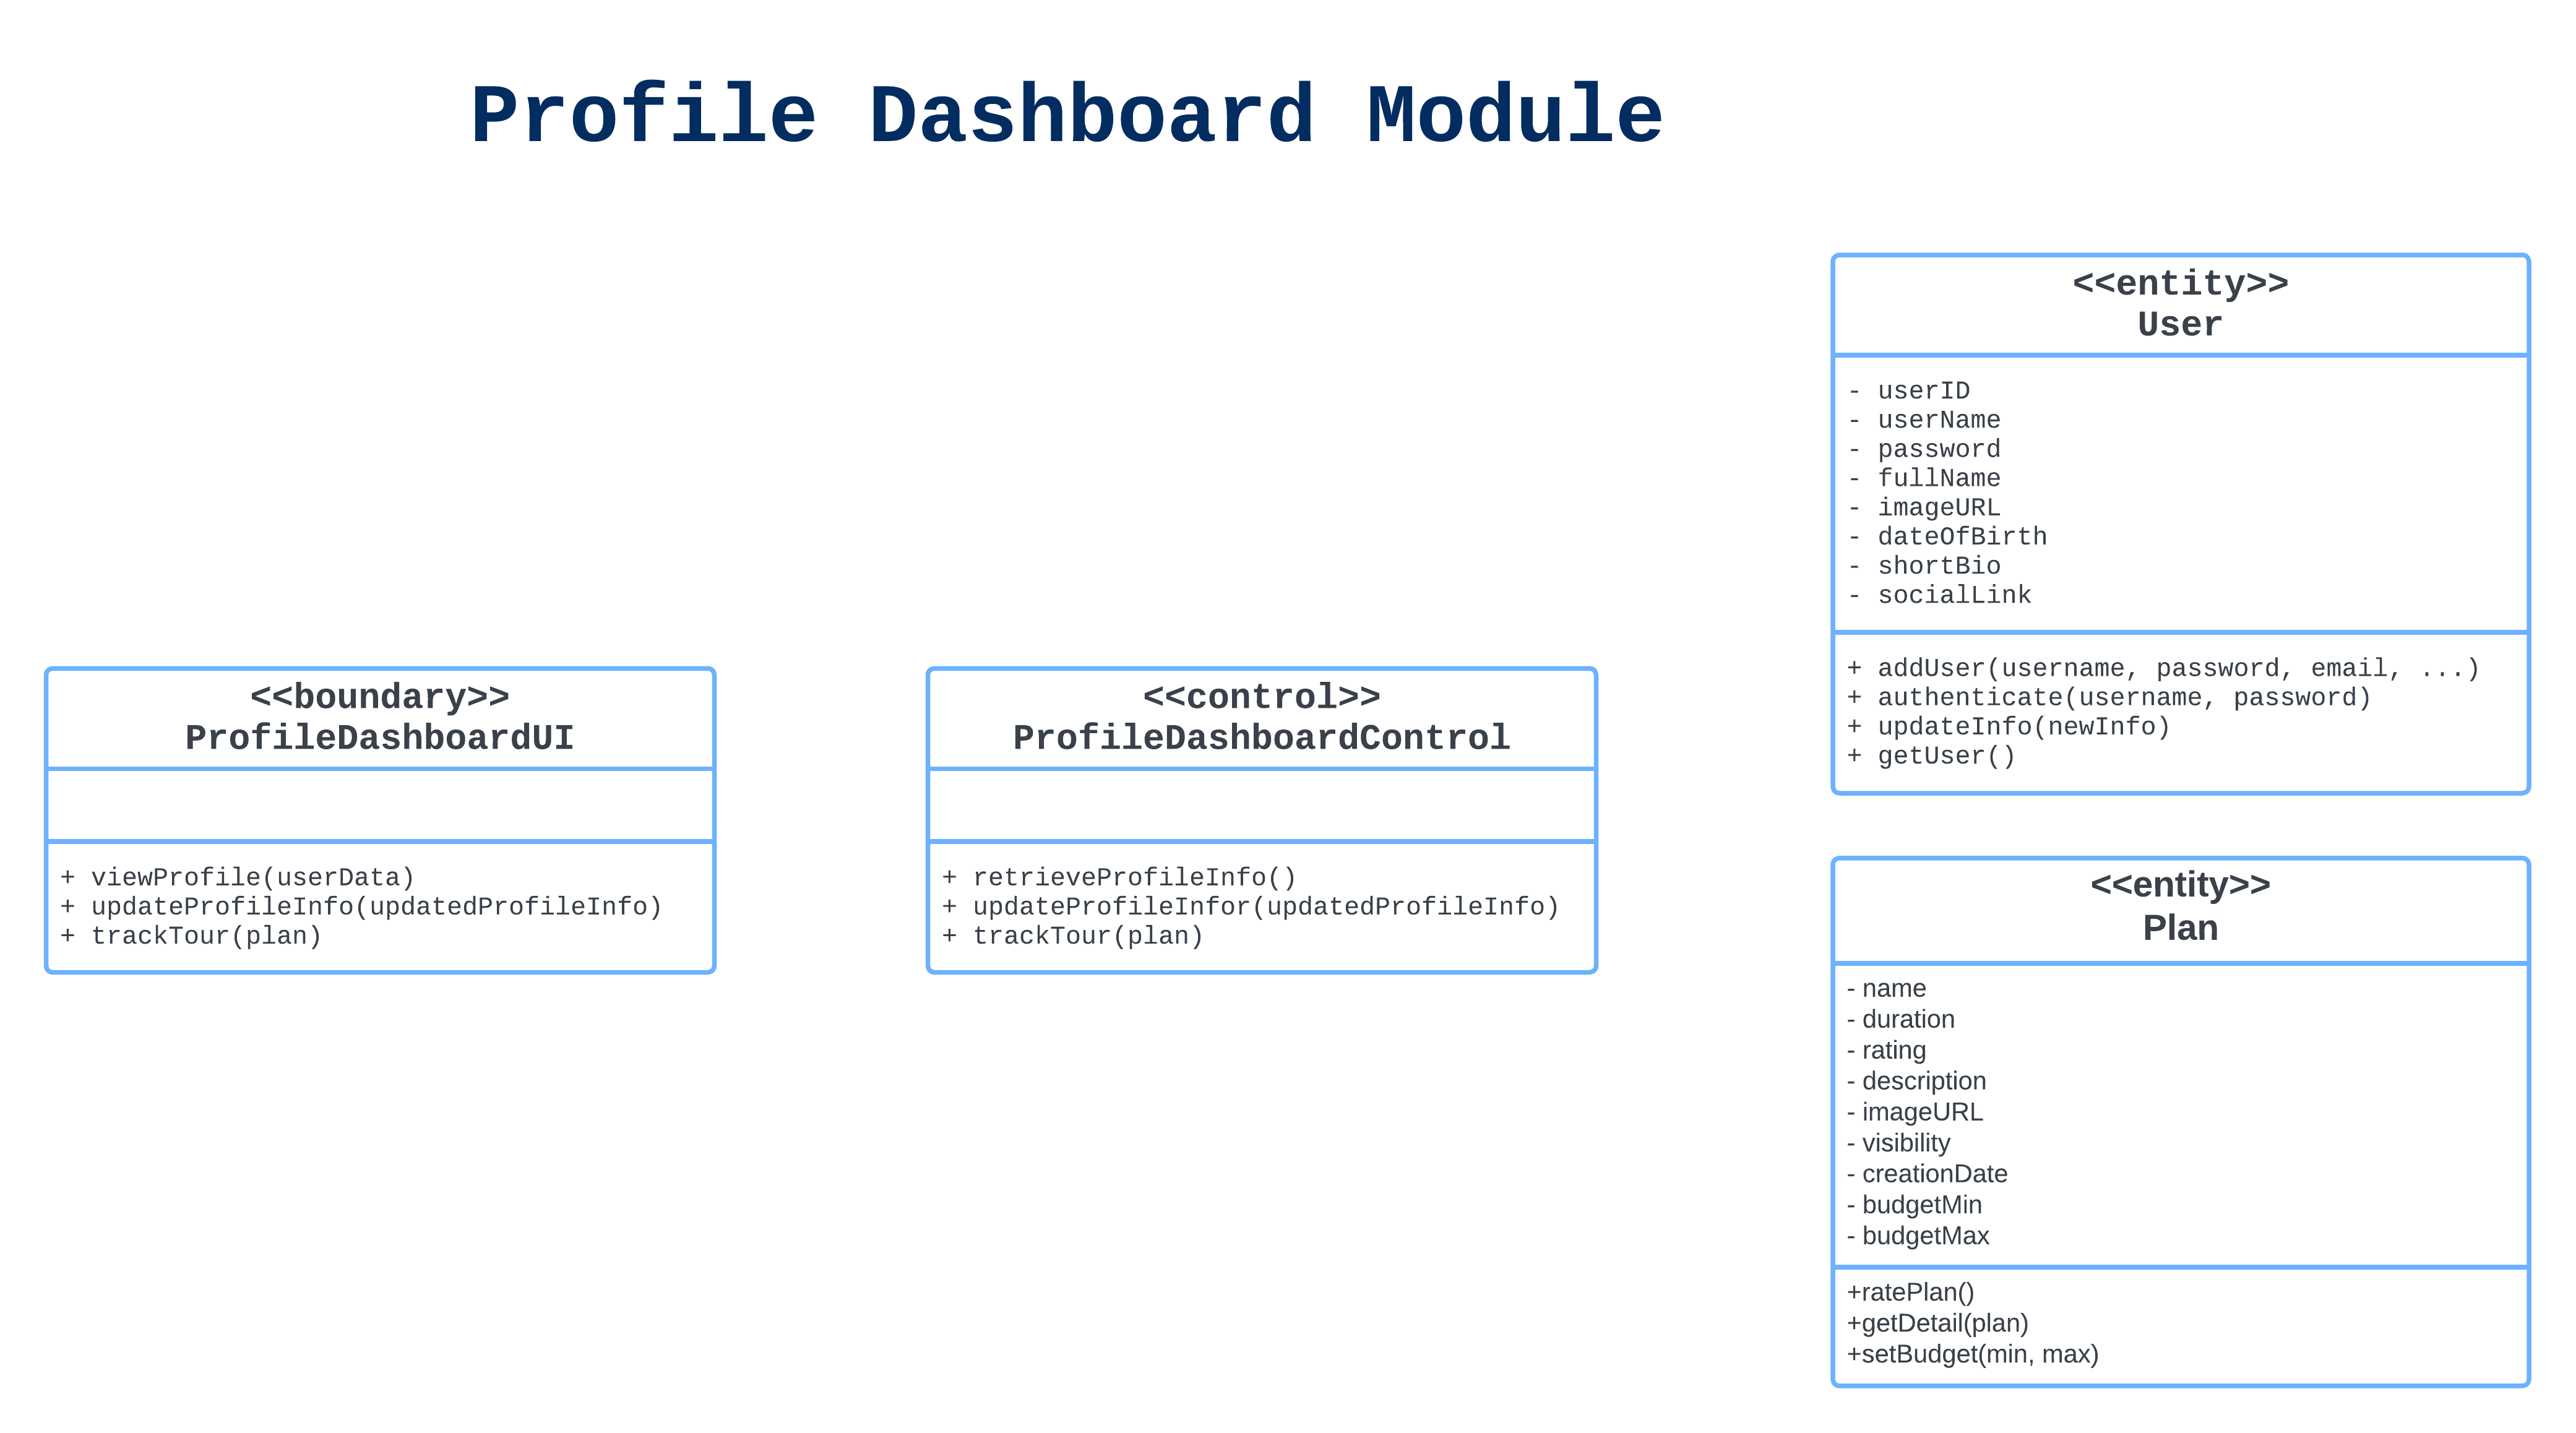
\includegraphics[width=0.85\textwidth]{Class Diagram/Profile Dashboard.png}
        \label{fig:ClassDash}
    \caption{Class Diagram - Profile Dashboard}
\end{figure}

\newpage
\subsection{Destinations}
\begin{figure}[H]
    \centering
        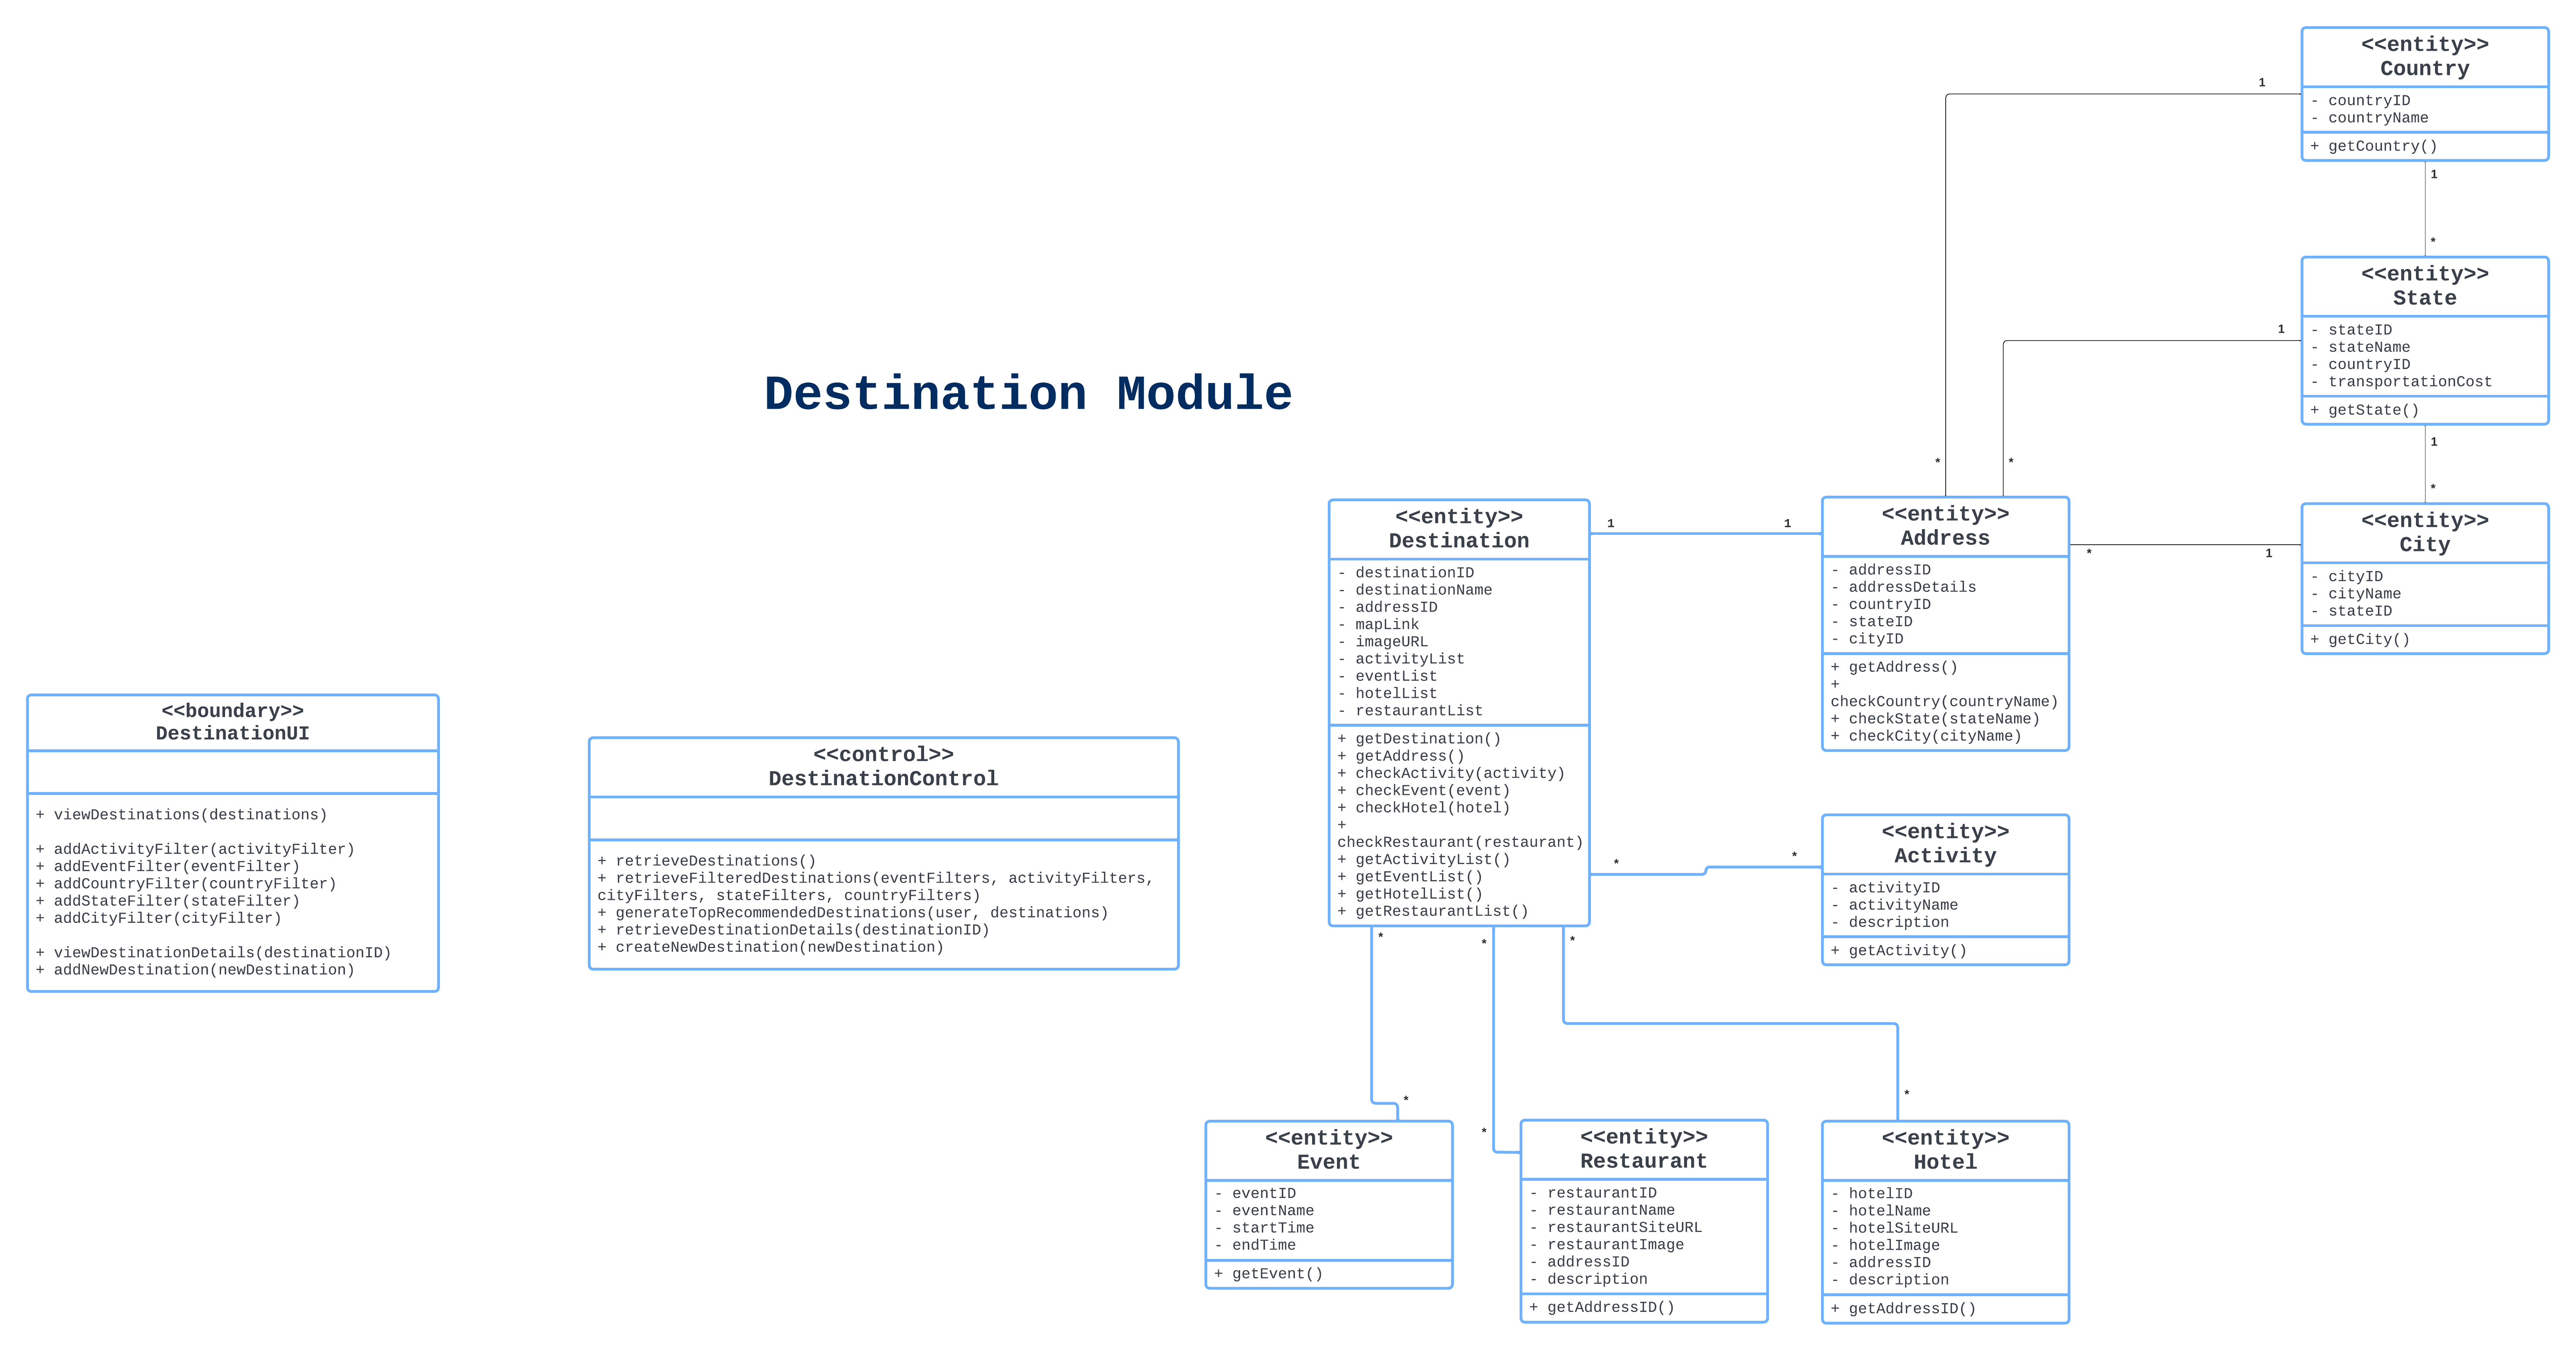
\includegraphics[width=0.85\textwidth]{Class Diagram/Destinations.png}
        \label{fig:ClassDest}
    \caption{Class Diagram - Destinations}
\end{figure}

\subsection{Destination Details}
\begin{figure}[H]
    \centering
        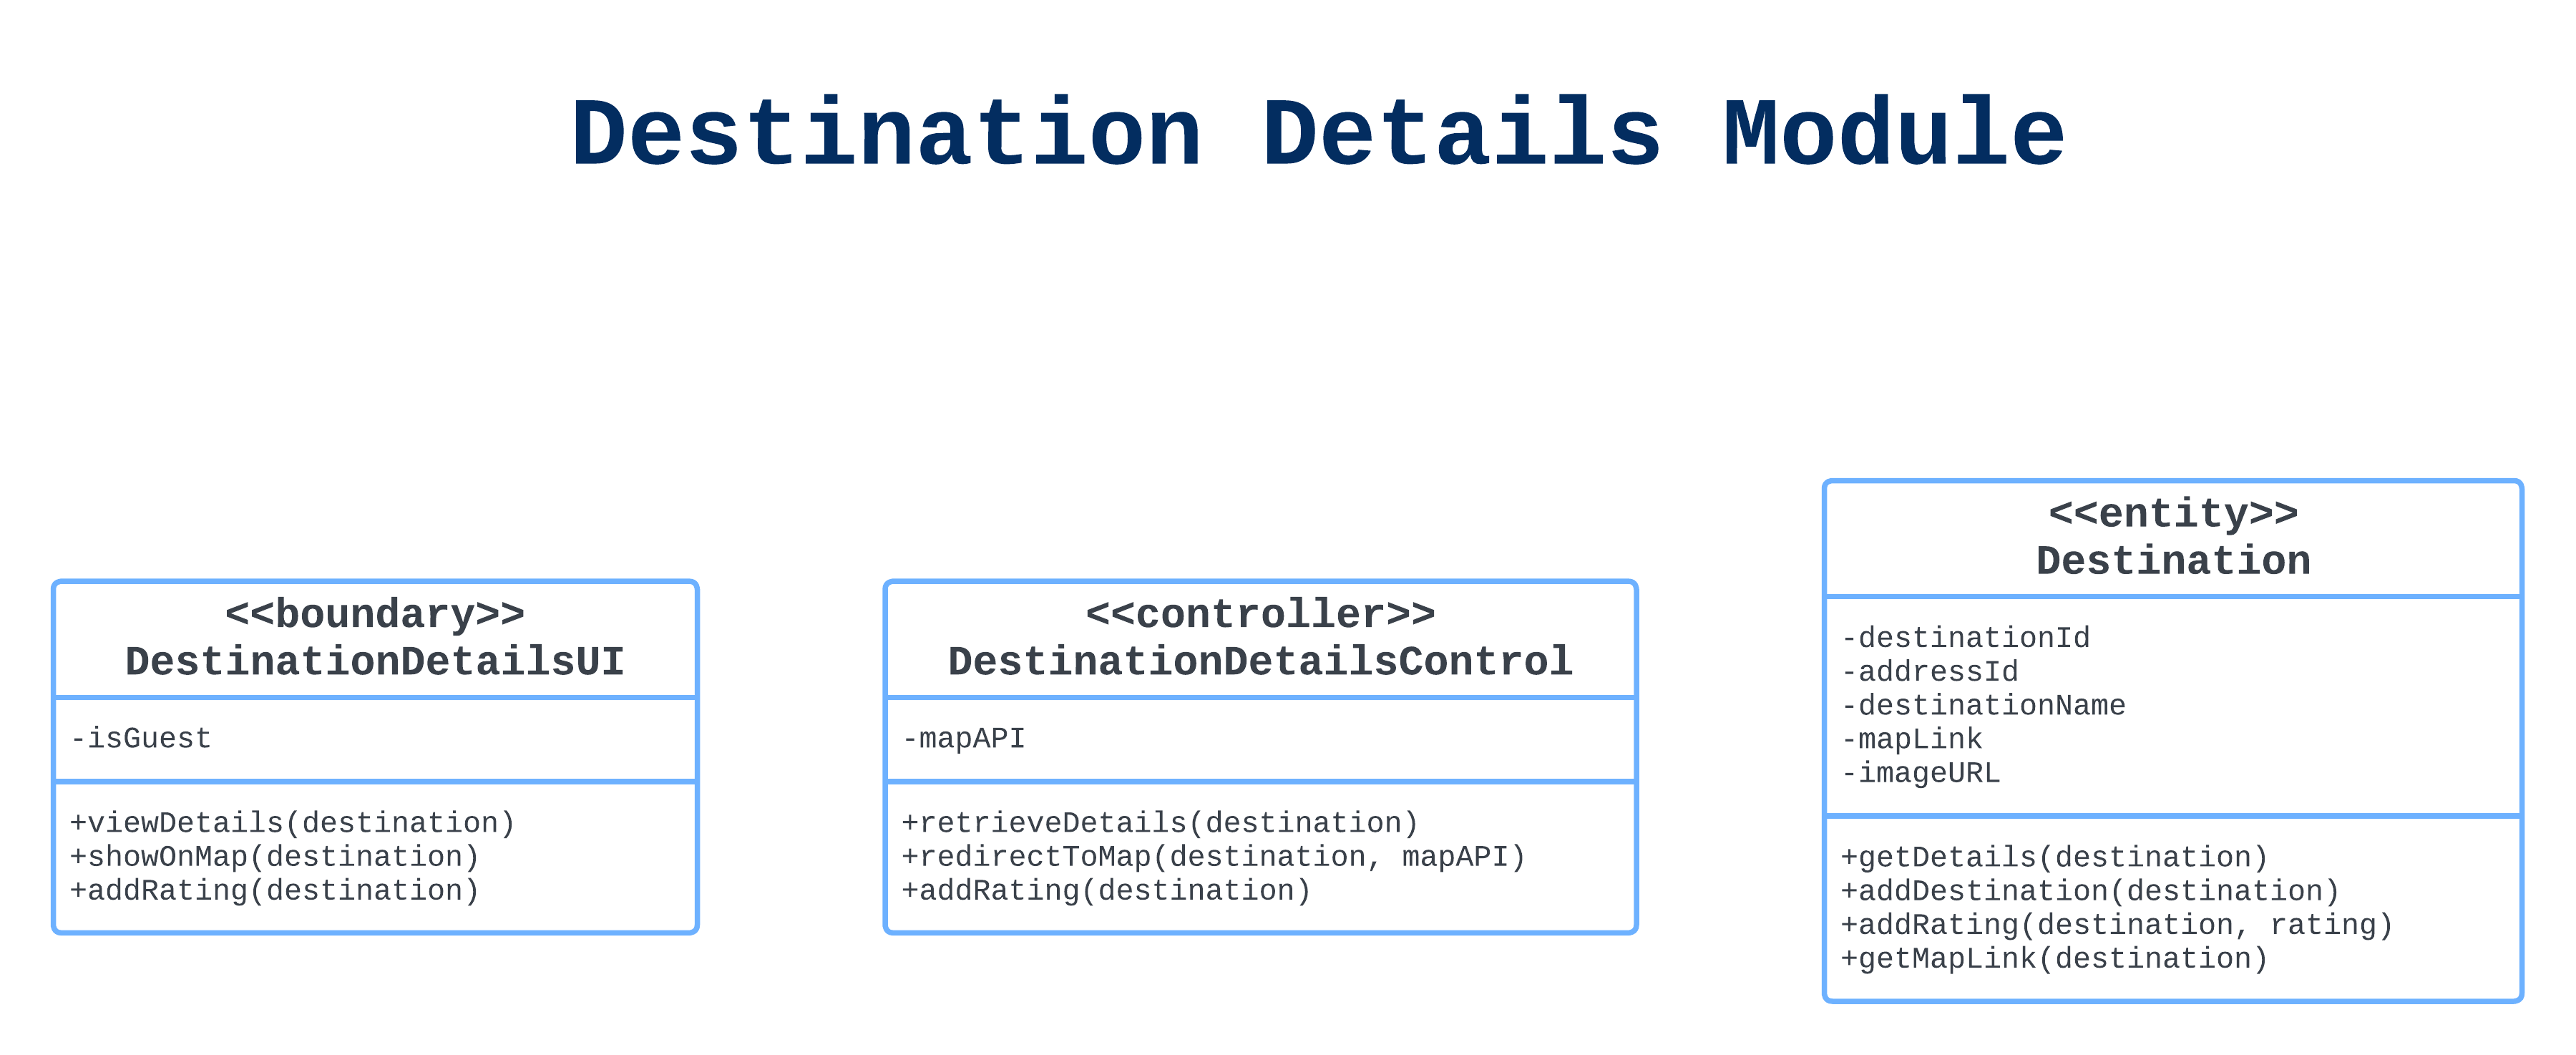
\includegraphics[width=0.85\textwidth]{Class Diagram/Destination Details.png}
        \label{fig:ClassDestDetails}
    \caption{Class Diagram - Destination Details}
\end{figure}

\newpage
\subsection{Plans}
\begin{figure}[H]
    \centering
        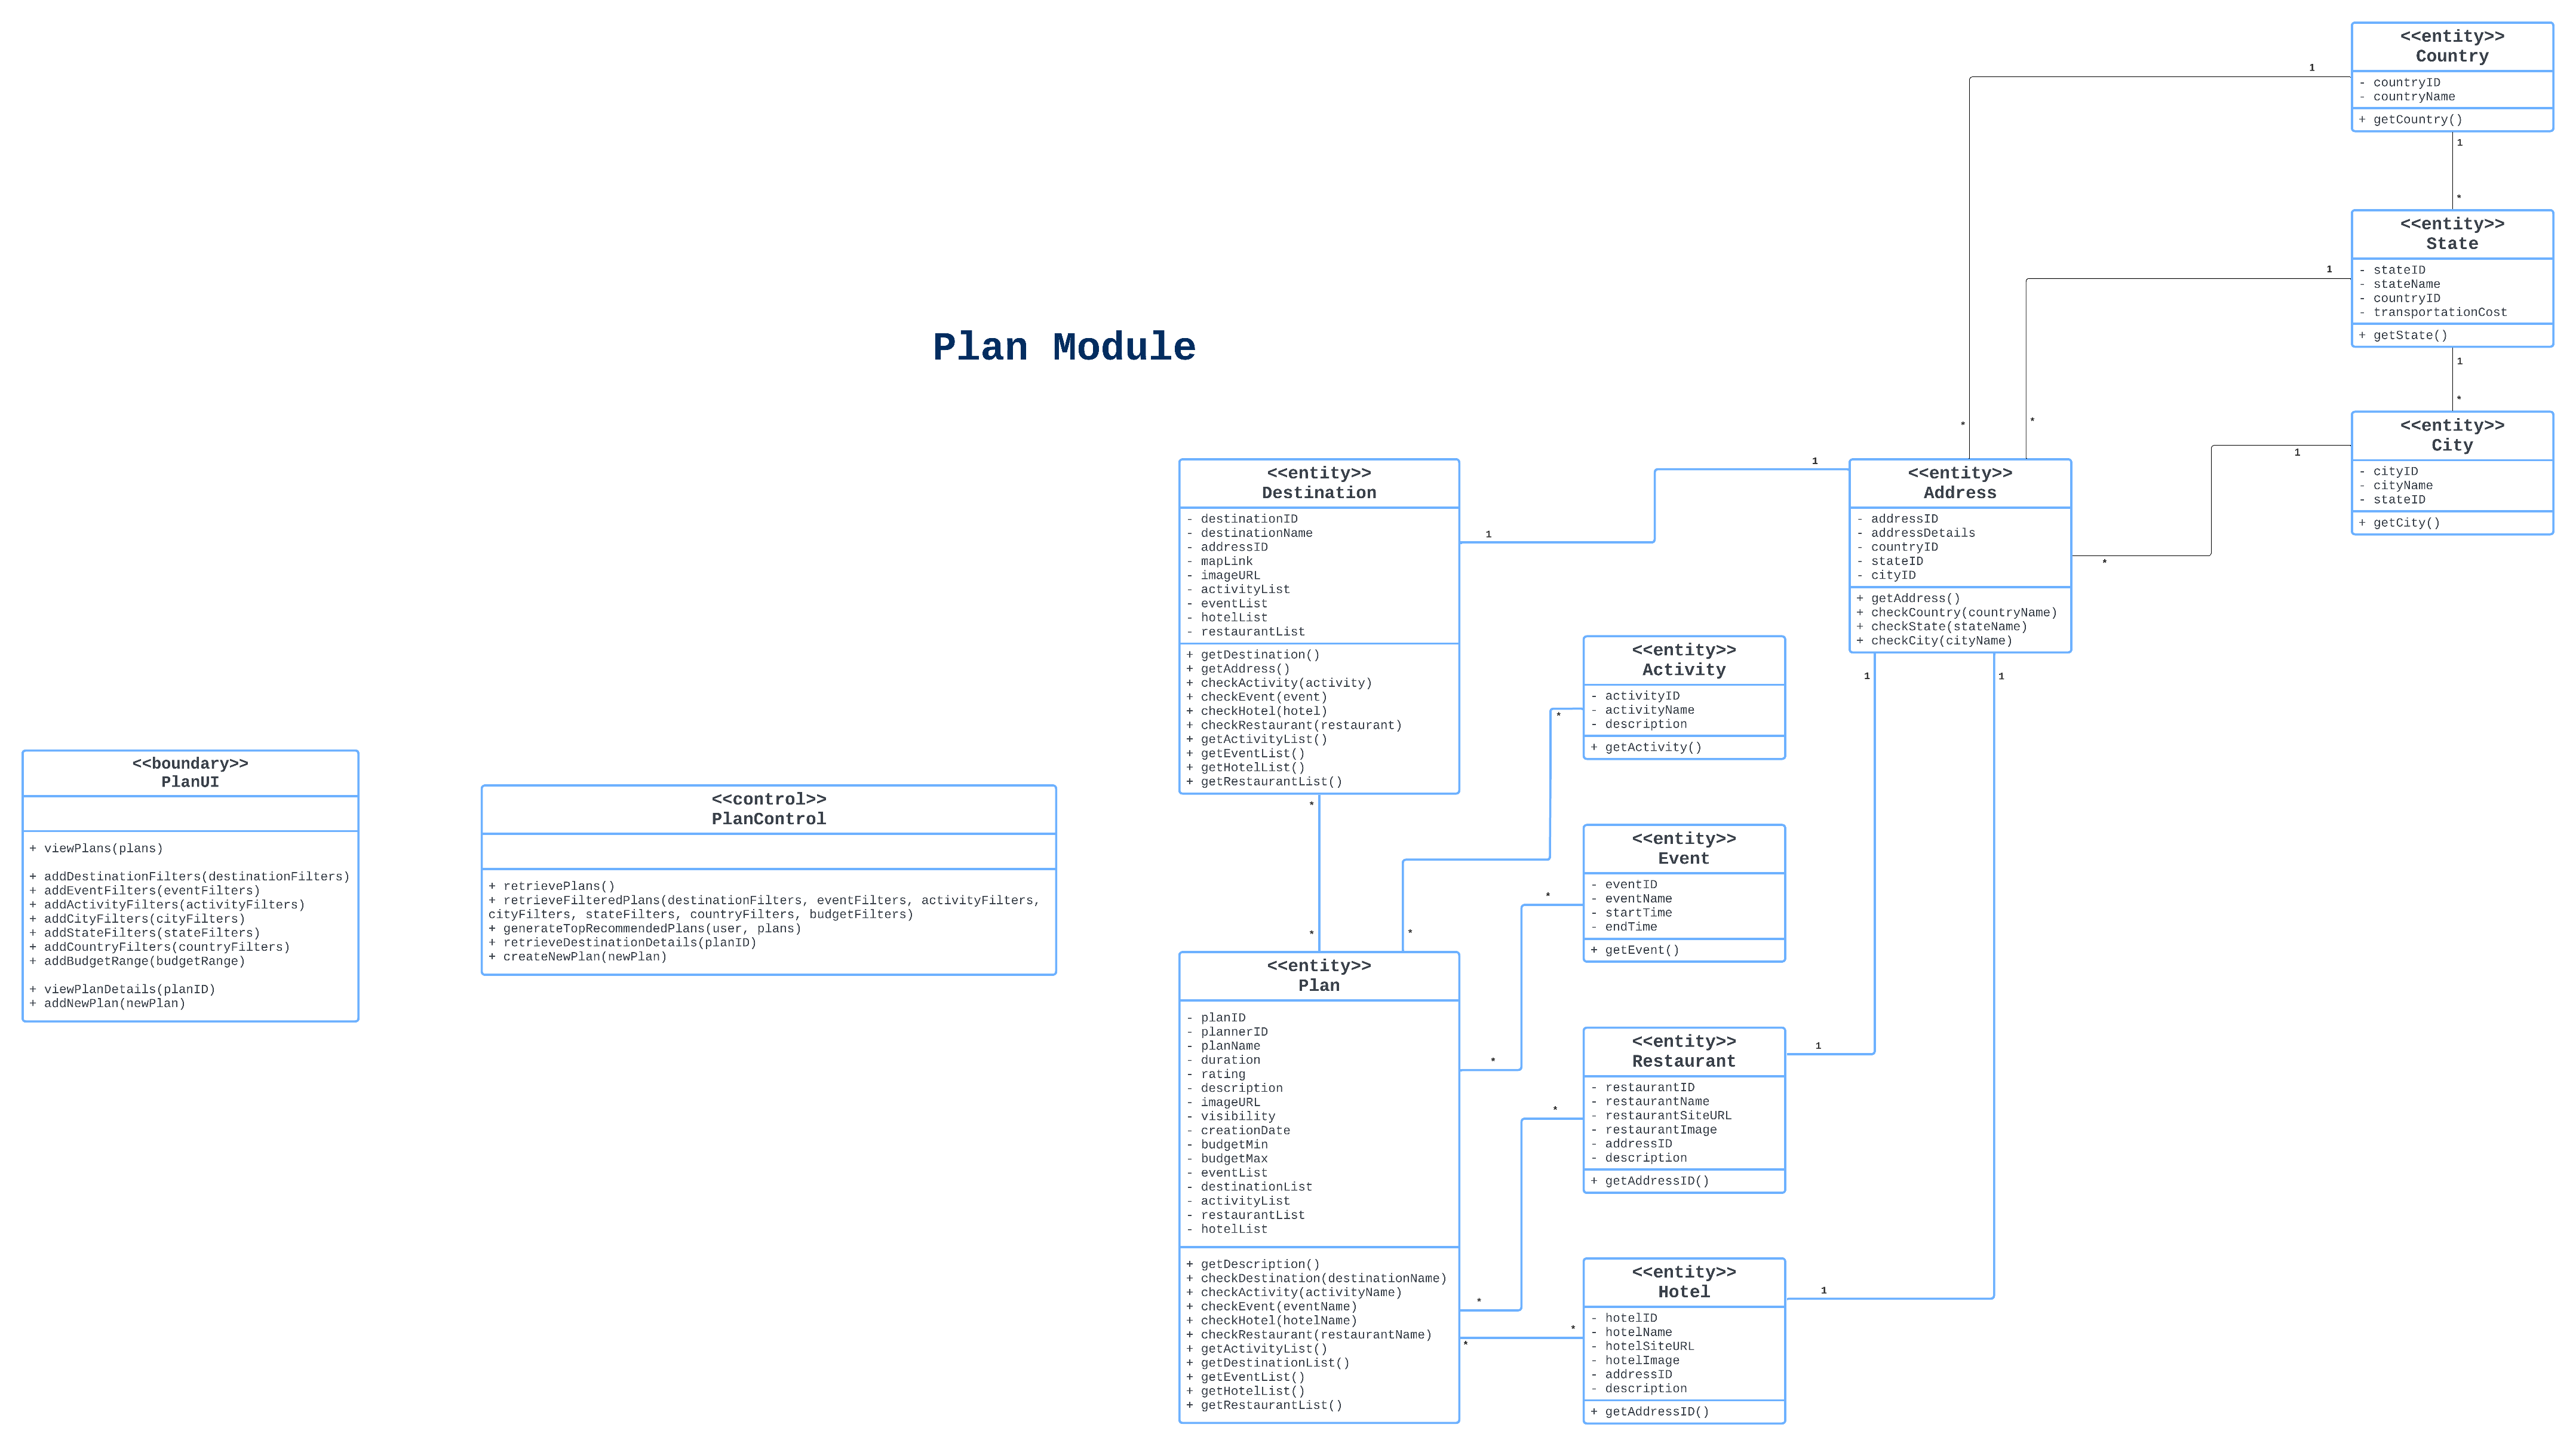
\includegraphics[width=0.85\textwidth]{Class Diagram/Plans.png}
        \label{fig:ClassPlans}
    \caption{Class Diagram - Plans}
\end{figure}

\subsection{Plan Details}
\begin{figure}[H]
    \centering
        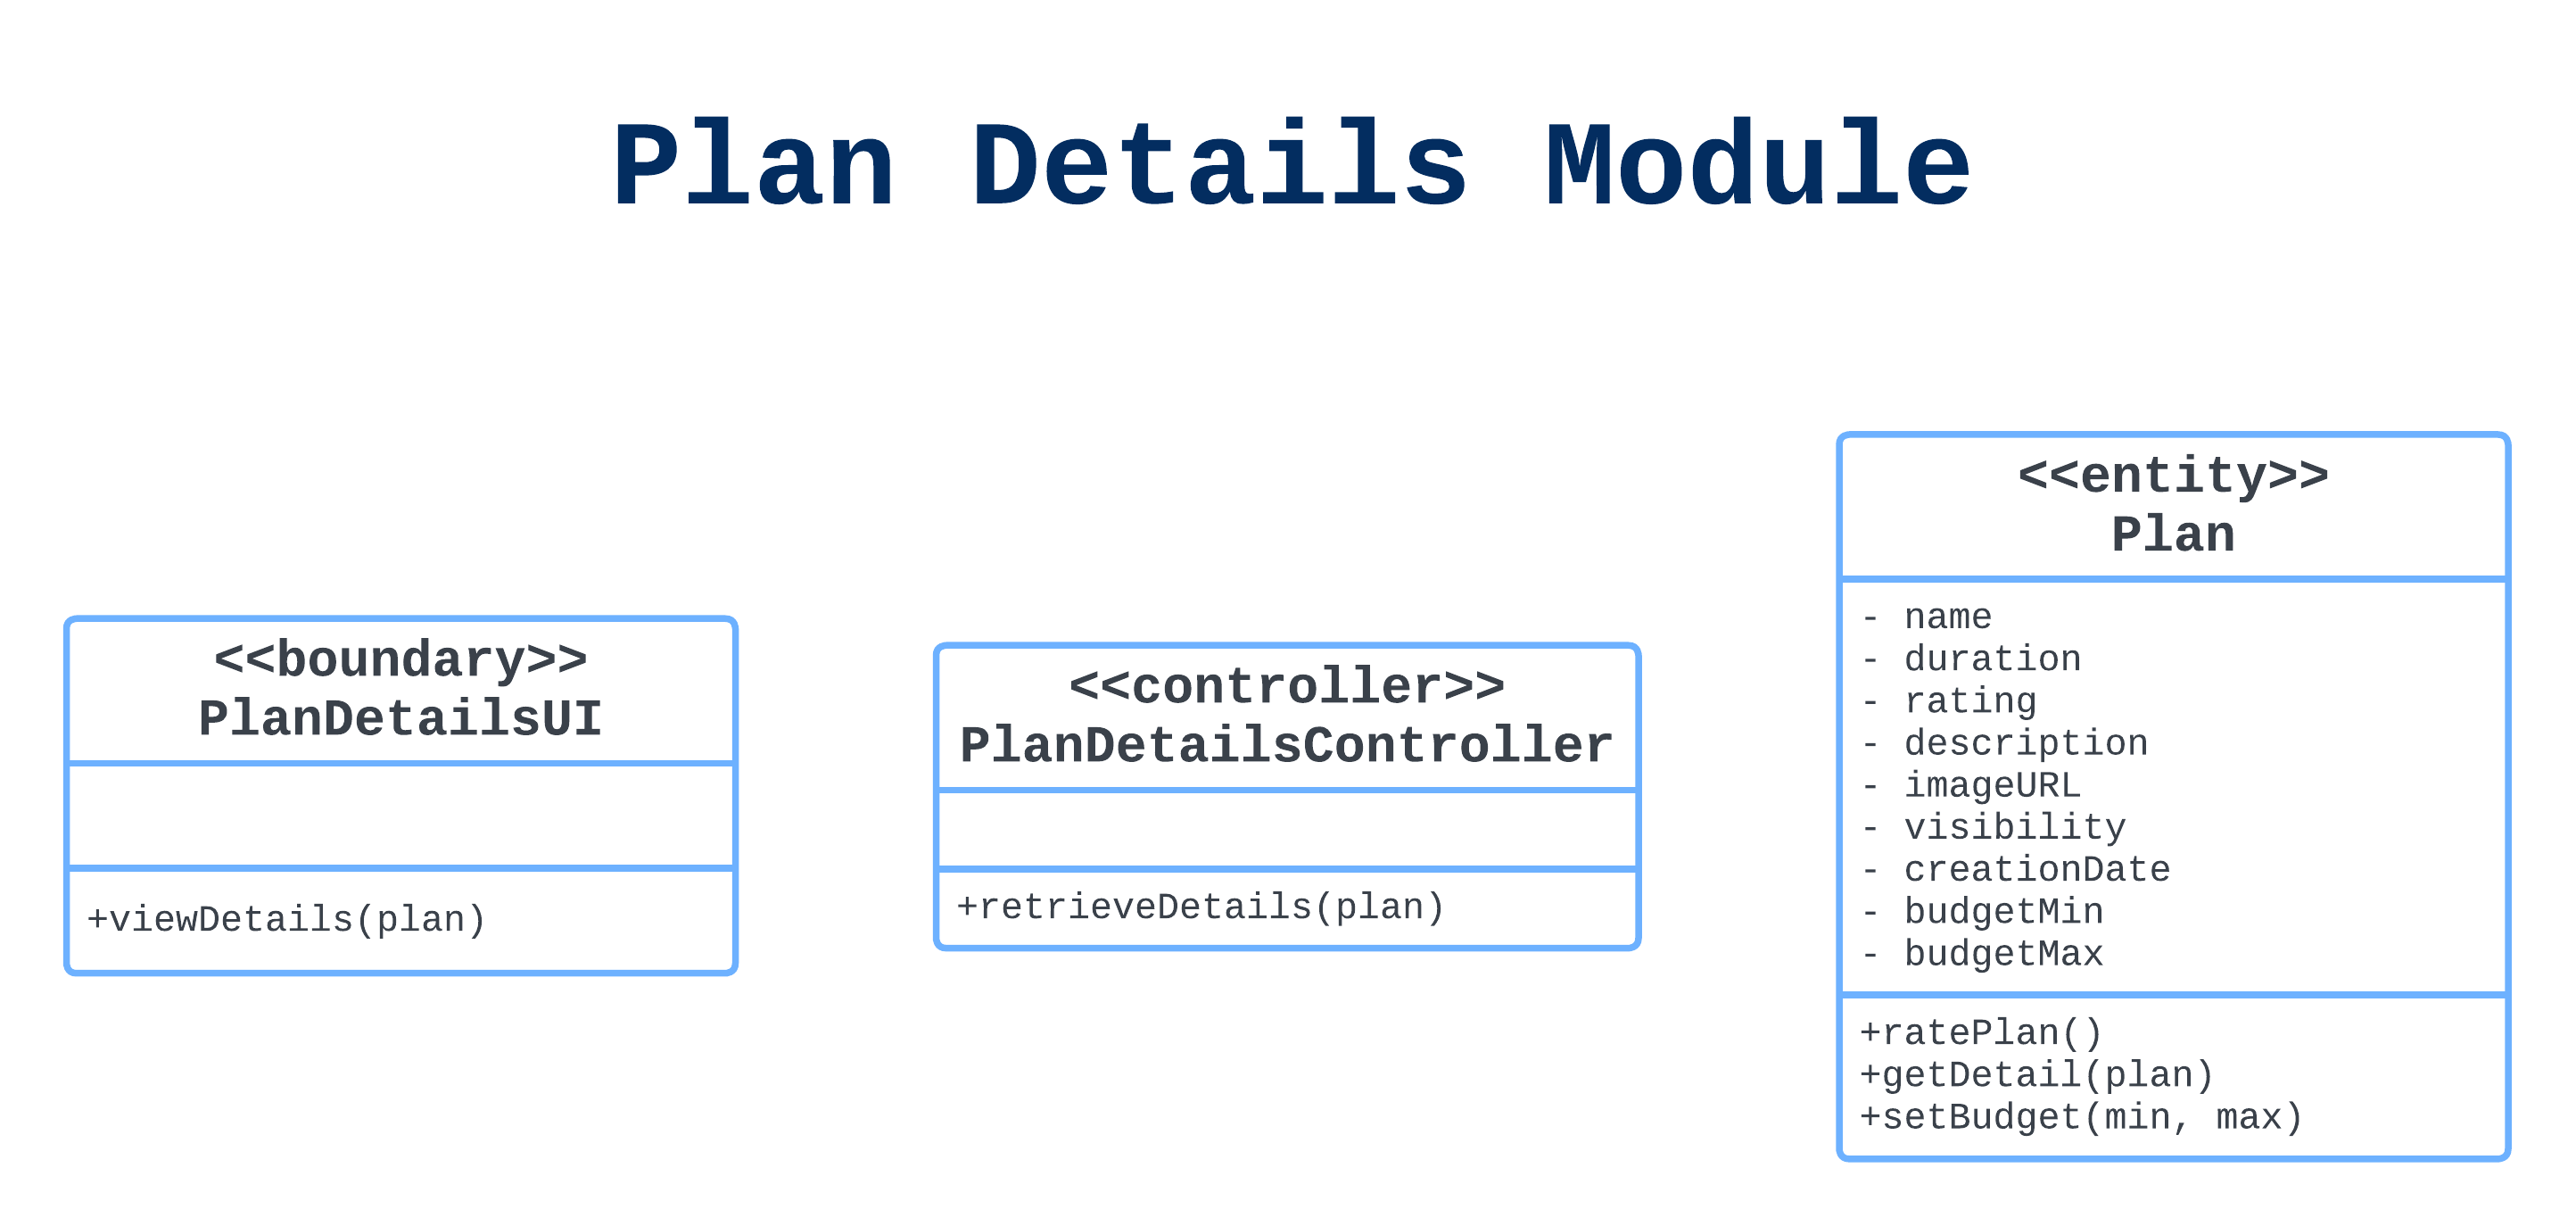
\includegraphics[width=0.85\textwidth]{Class Diagram/Plan Details.png}
        \label{fig:ClassPlanDetails}
    \caption{Class Diagram - Plan Details}
\end{figure}

\newpage
\subsection{Customize Plan}
\begin{figure}[H]
    \centering
        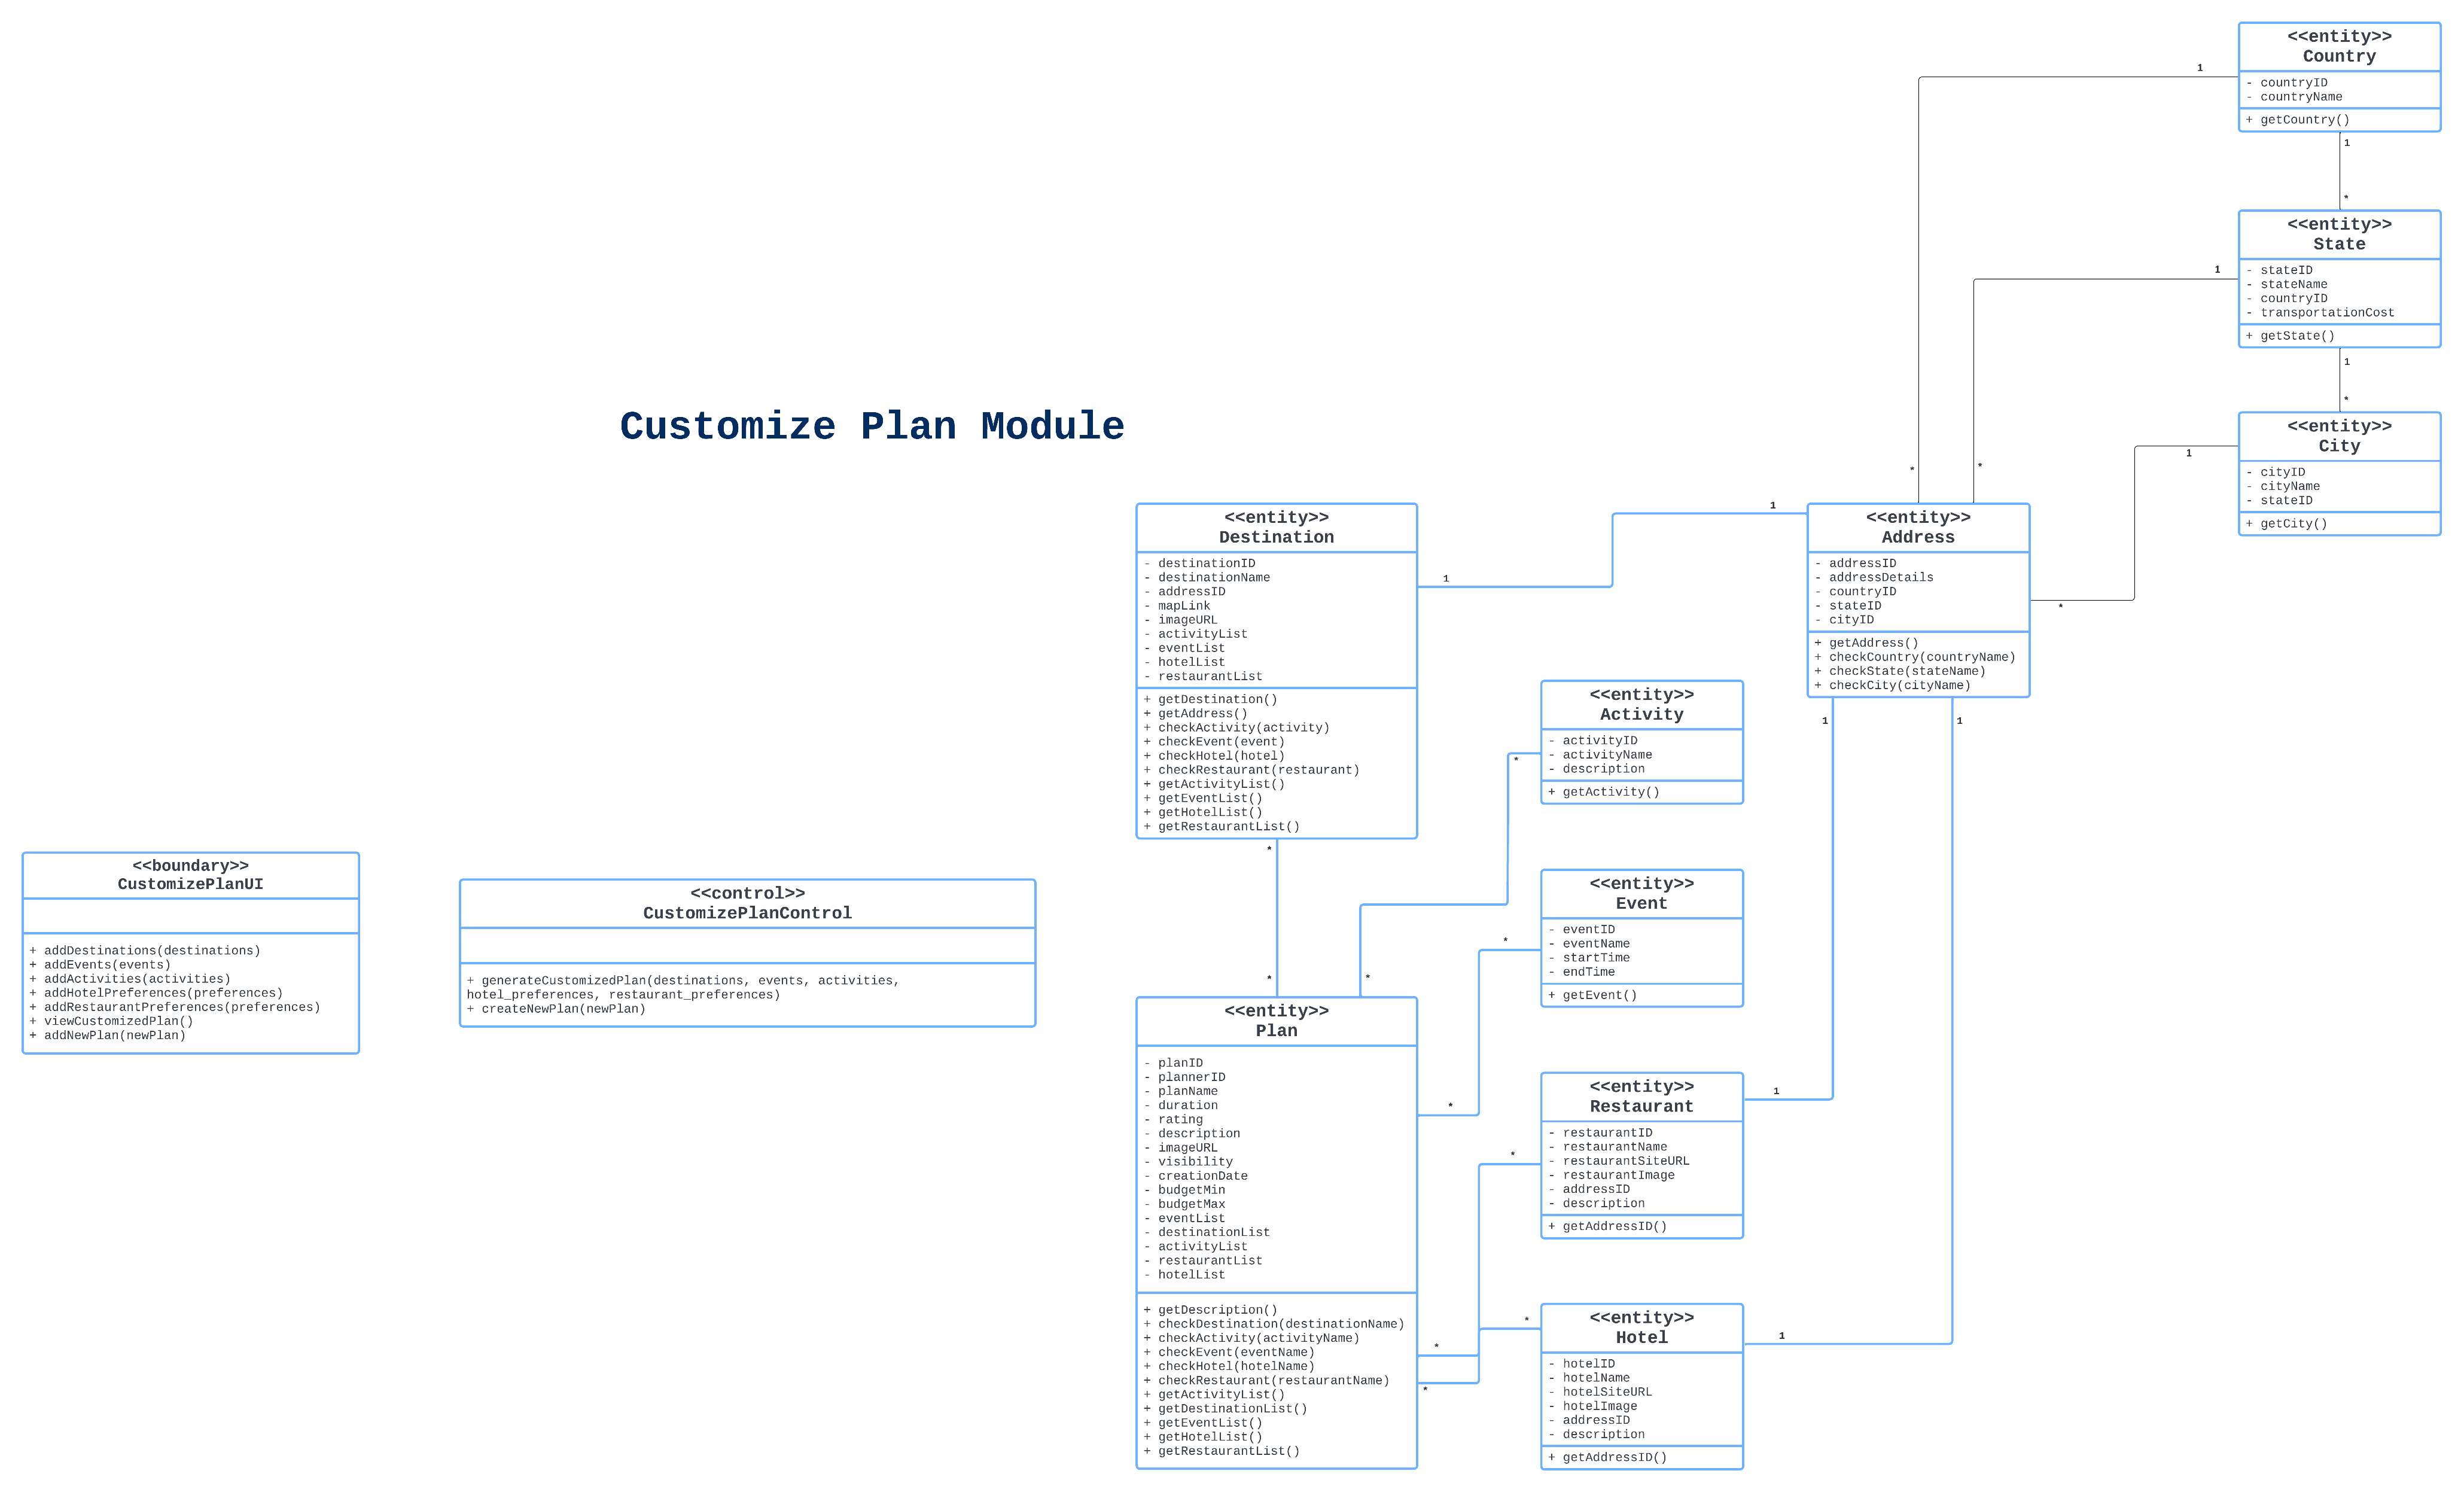
\includegraphics[width=0.85\textwidth]{Class Diagram/CustomizePlan.png}
        \label{fig:ClassCustomize}
    \caption{Class Diagram - Customize Plan}
\end{figure}

\subsection{Tours}
\begin{figure}[H]
    \centering
        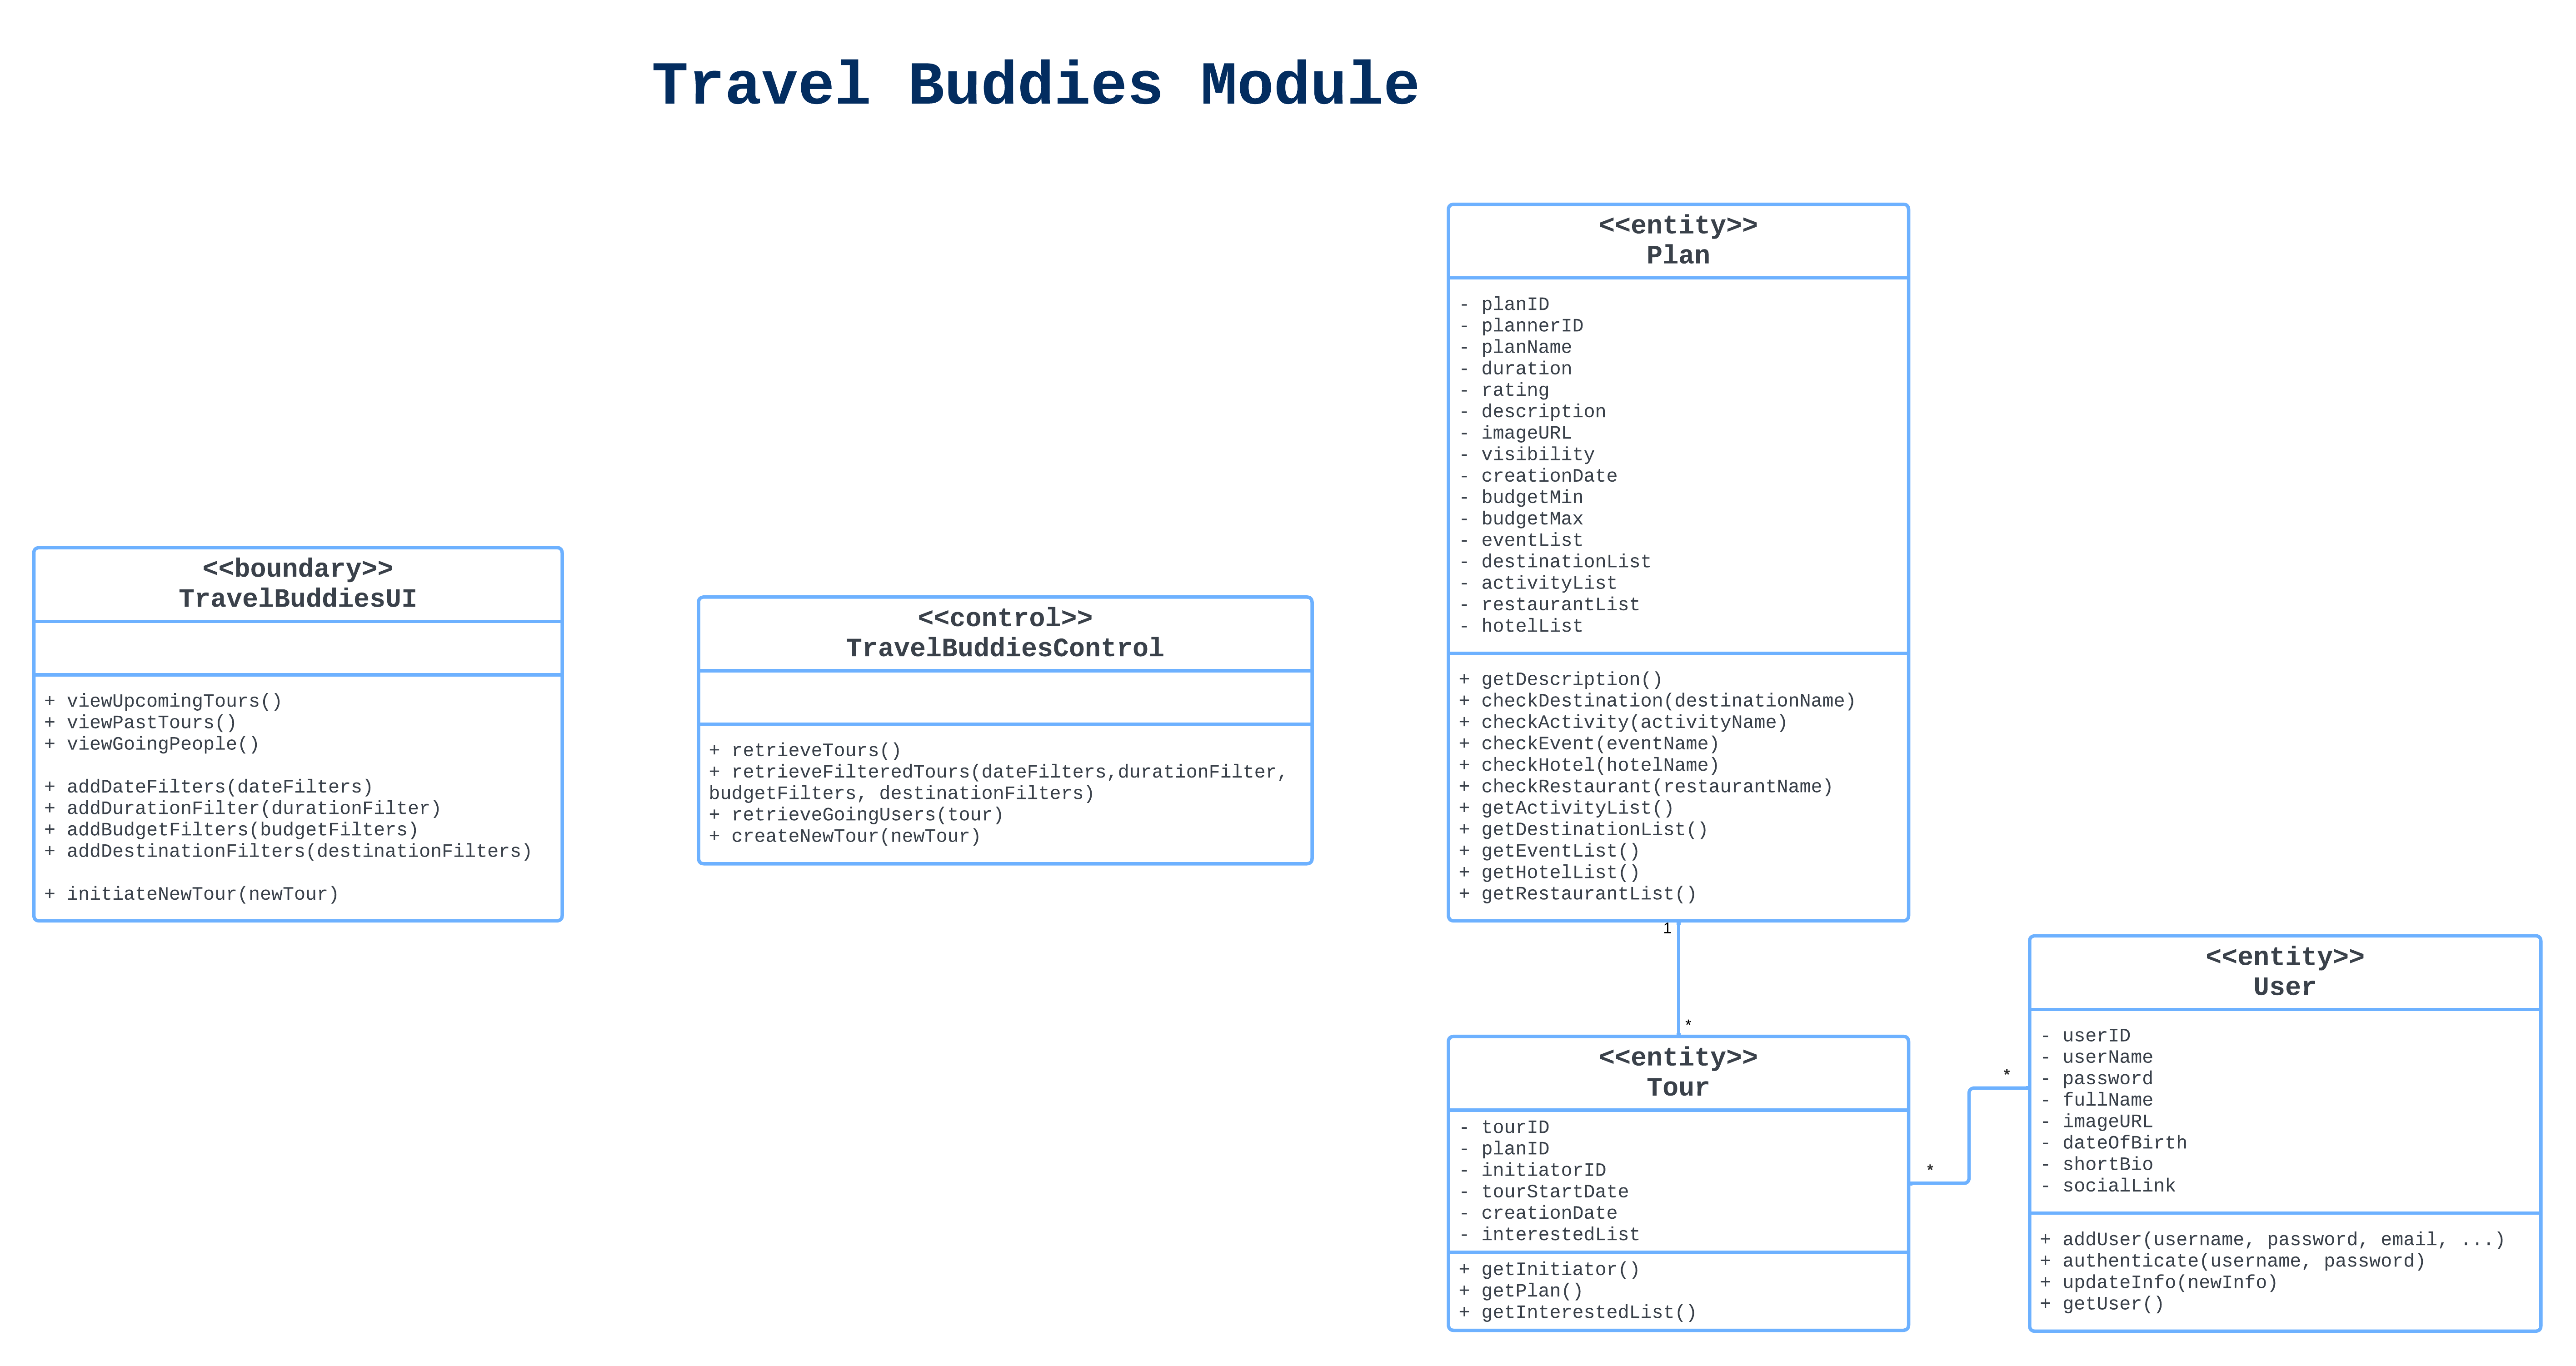
\includegraphics[width=0.85\textwidth]{Class Diagram/Travel Buddies.png}
        \label{fig:ClassTour}
    \caption{Class Diagram - Tours}
\end{figure}

\newpage

\section{Sequence Diagrams}
\subsection{Sign Up}
\begin{figure}[H]
    \centering
        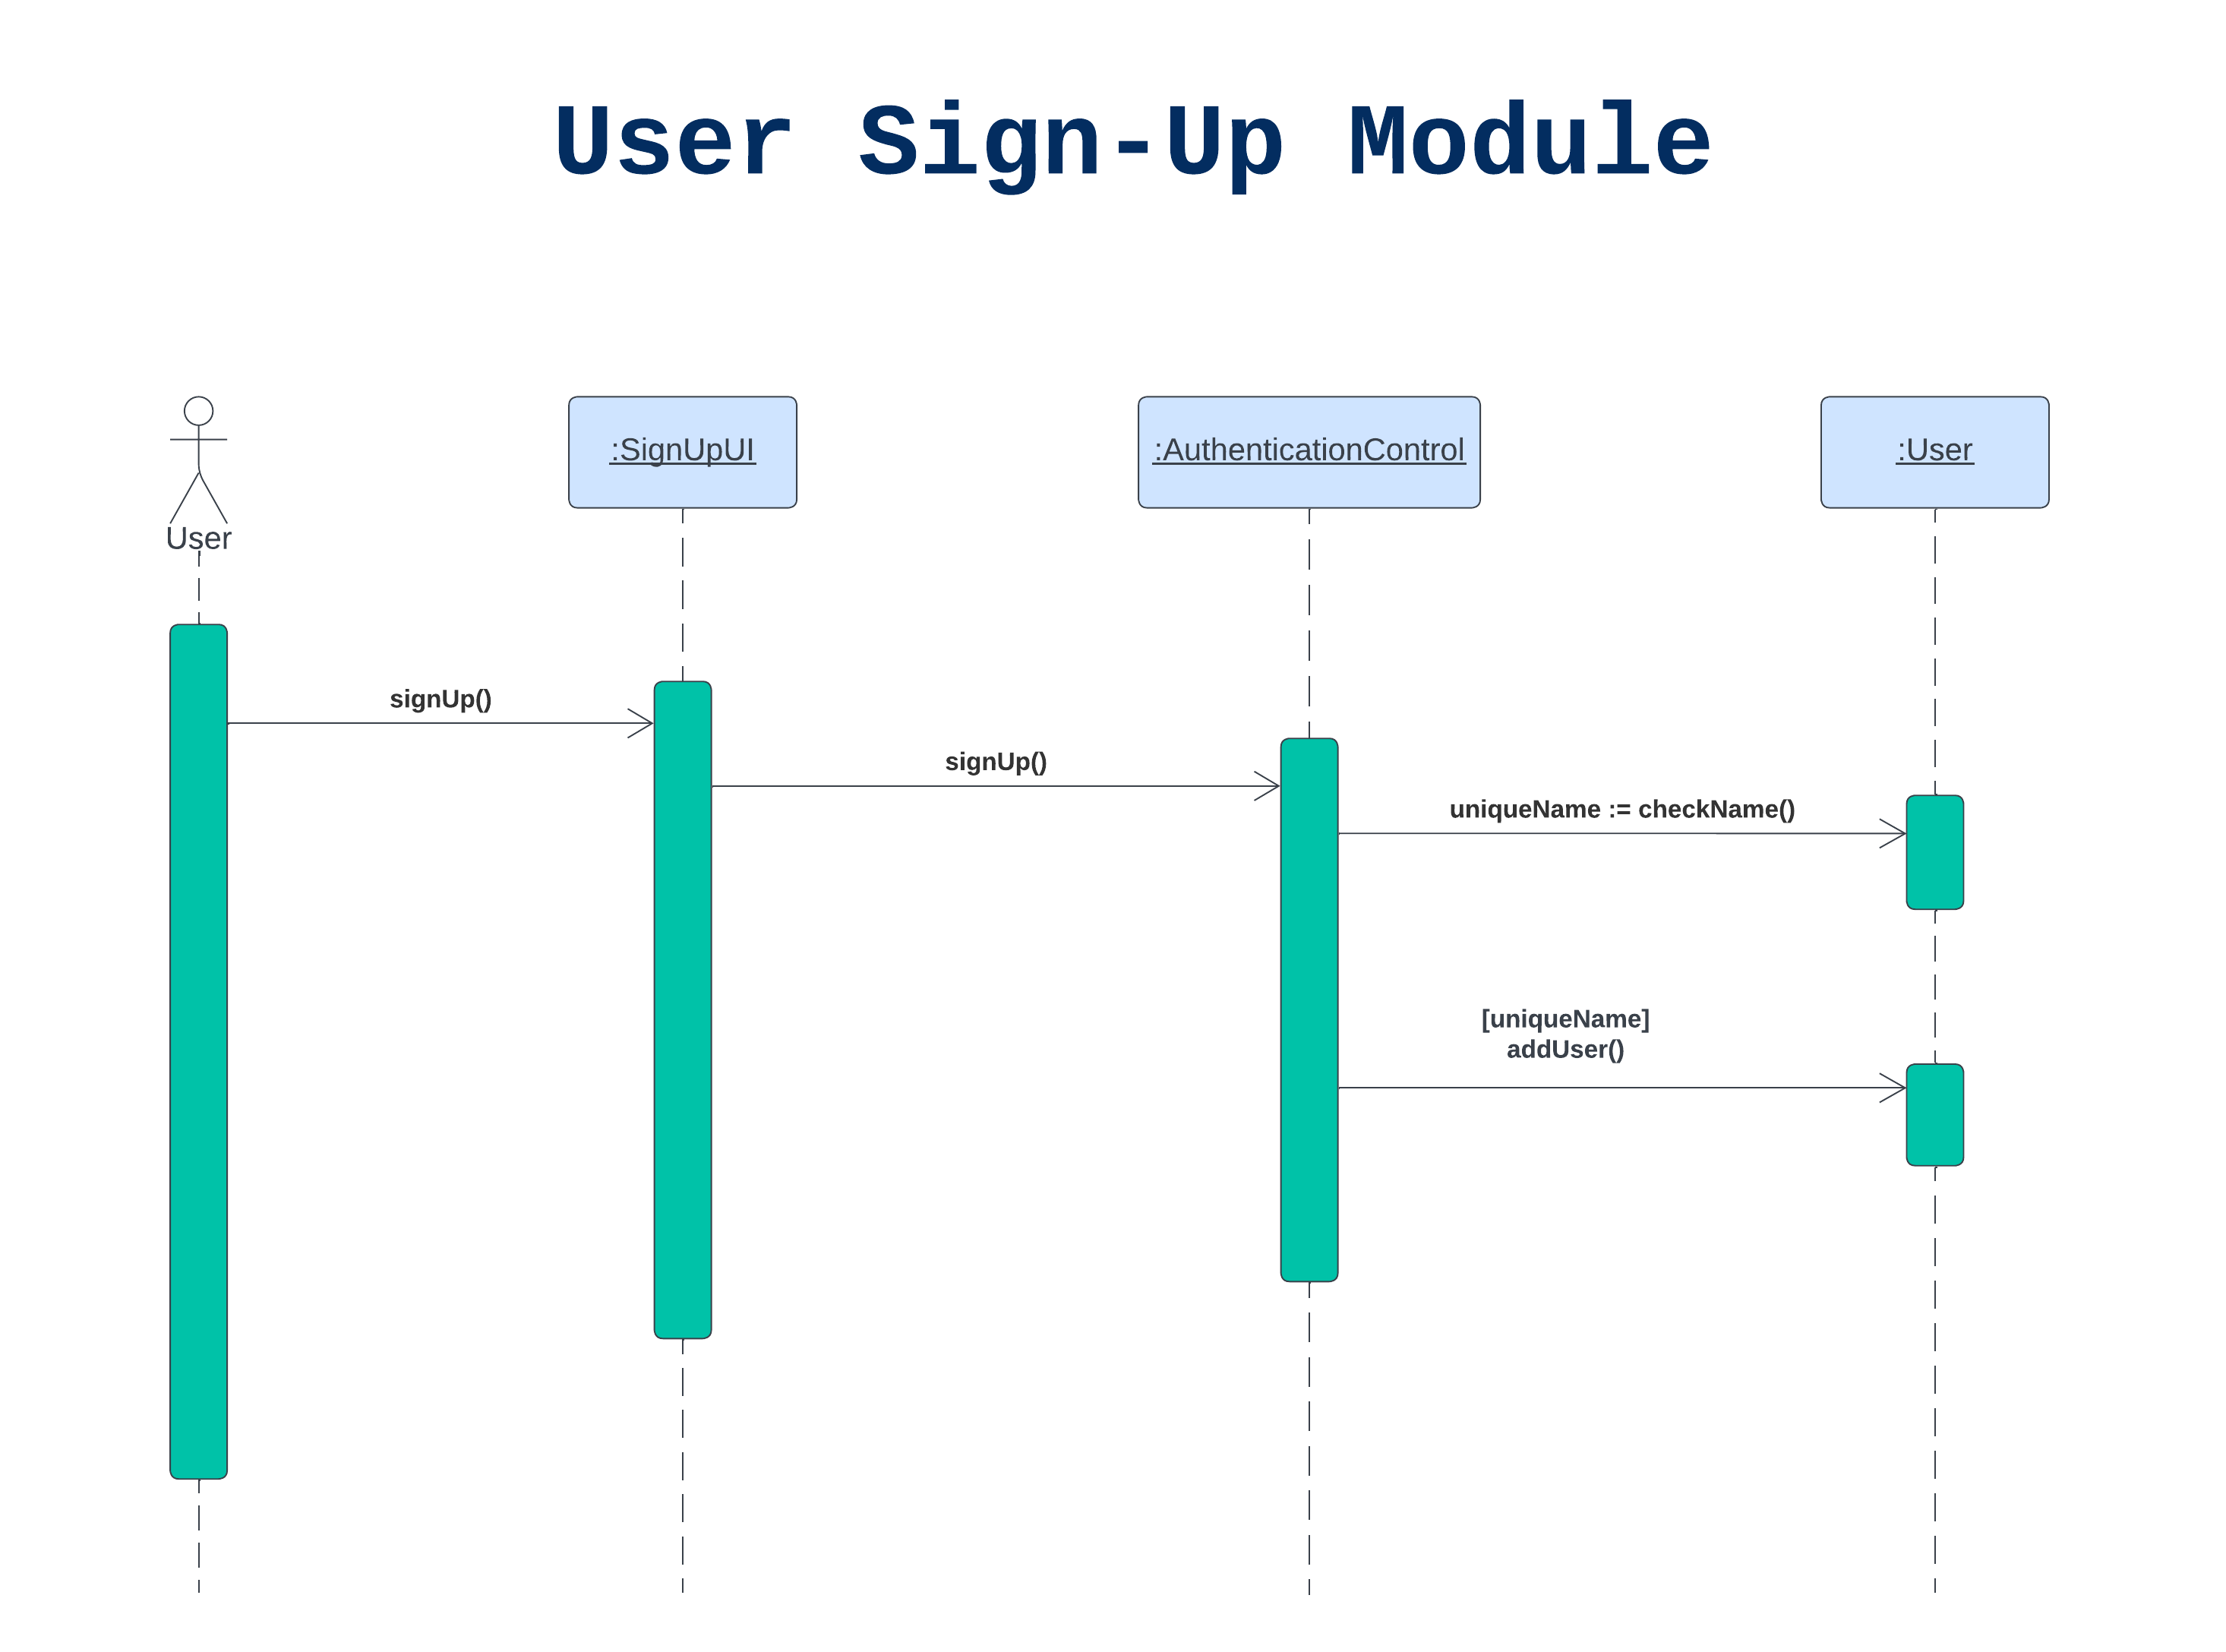
\includegraphics[width=\textwidth]{Sequence Diagram/Signup.png}
        \label{fig:SeqSign}
    \caption{Sequence Diagram - Sign Up}
\end{figure}

\newpage
\subsection{User Login}
\begin{figure}[H]
    \centering
        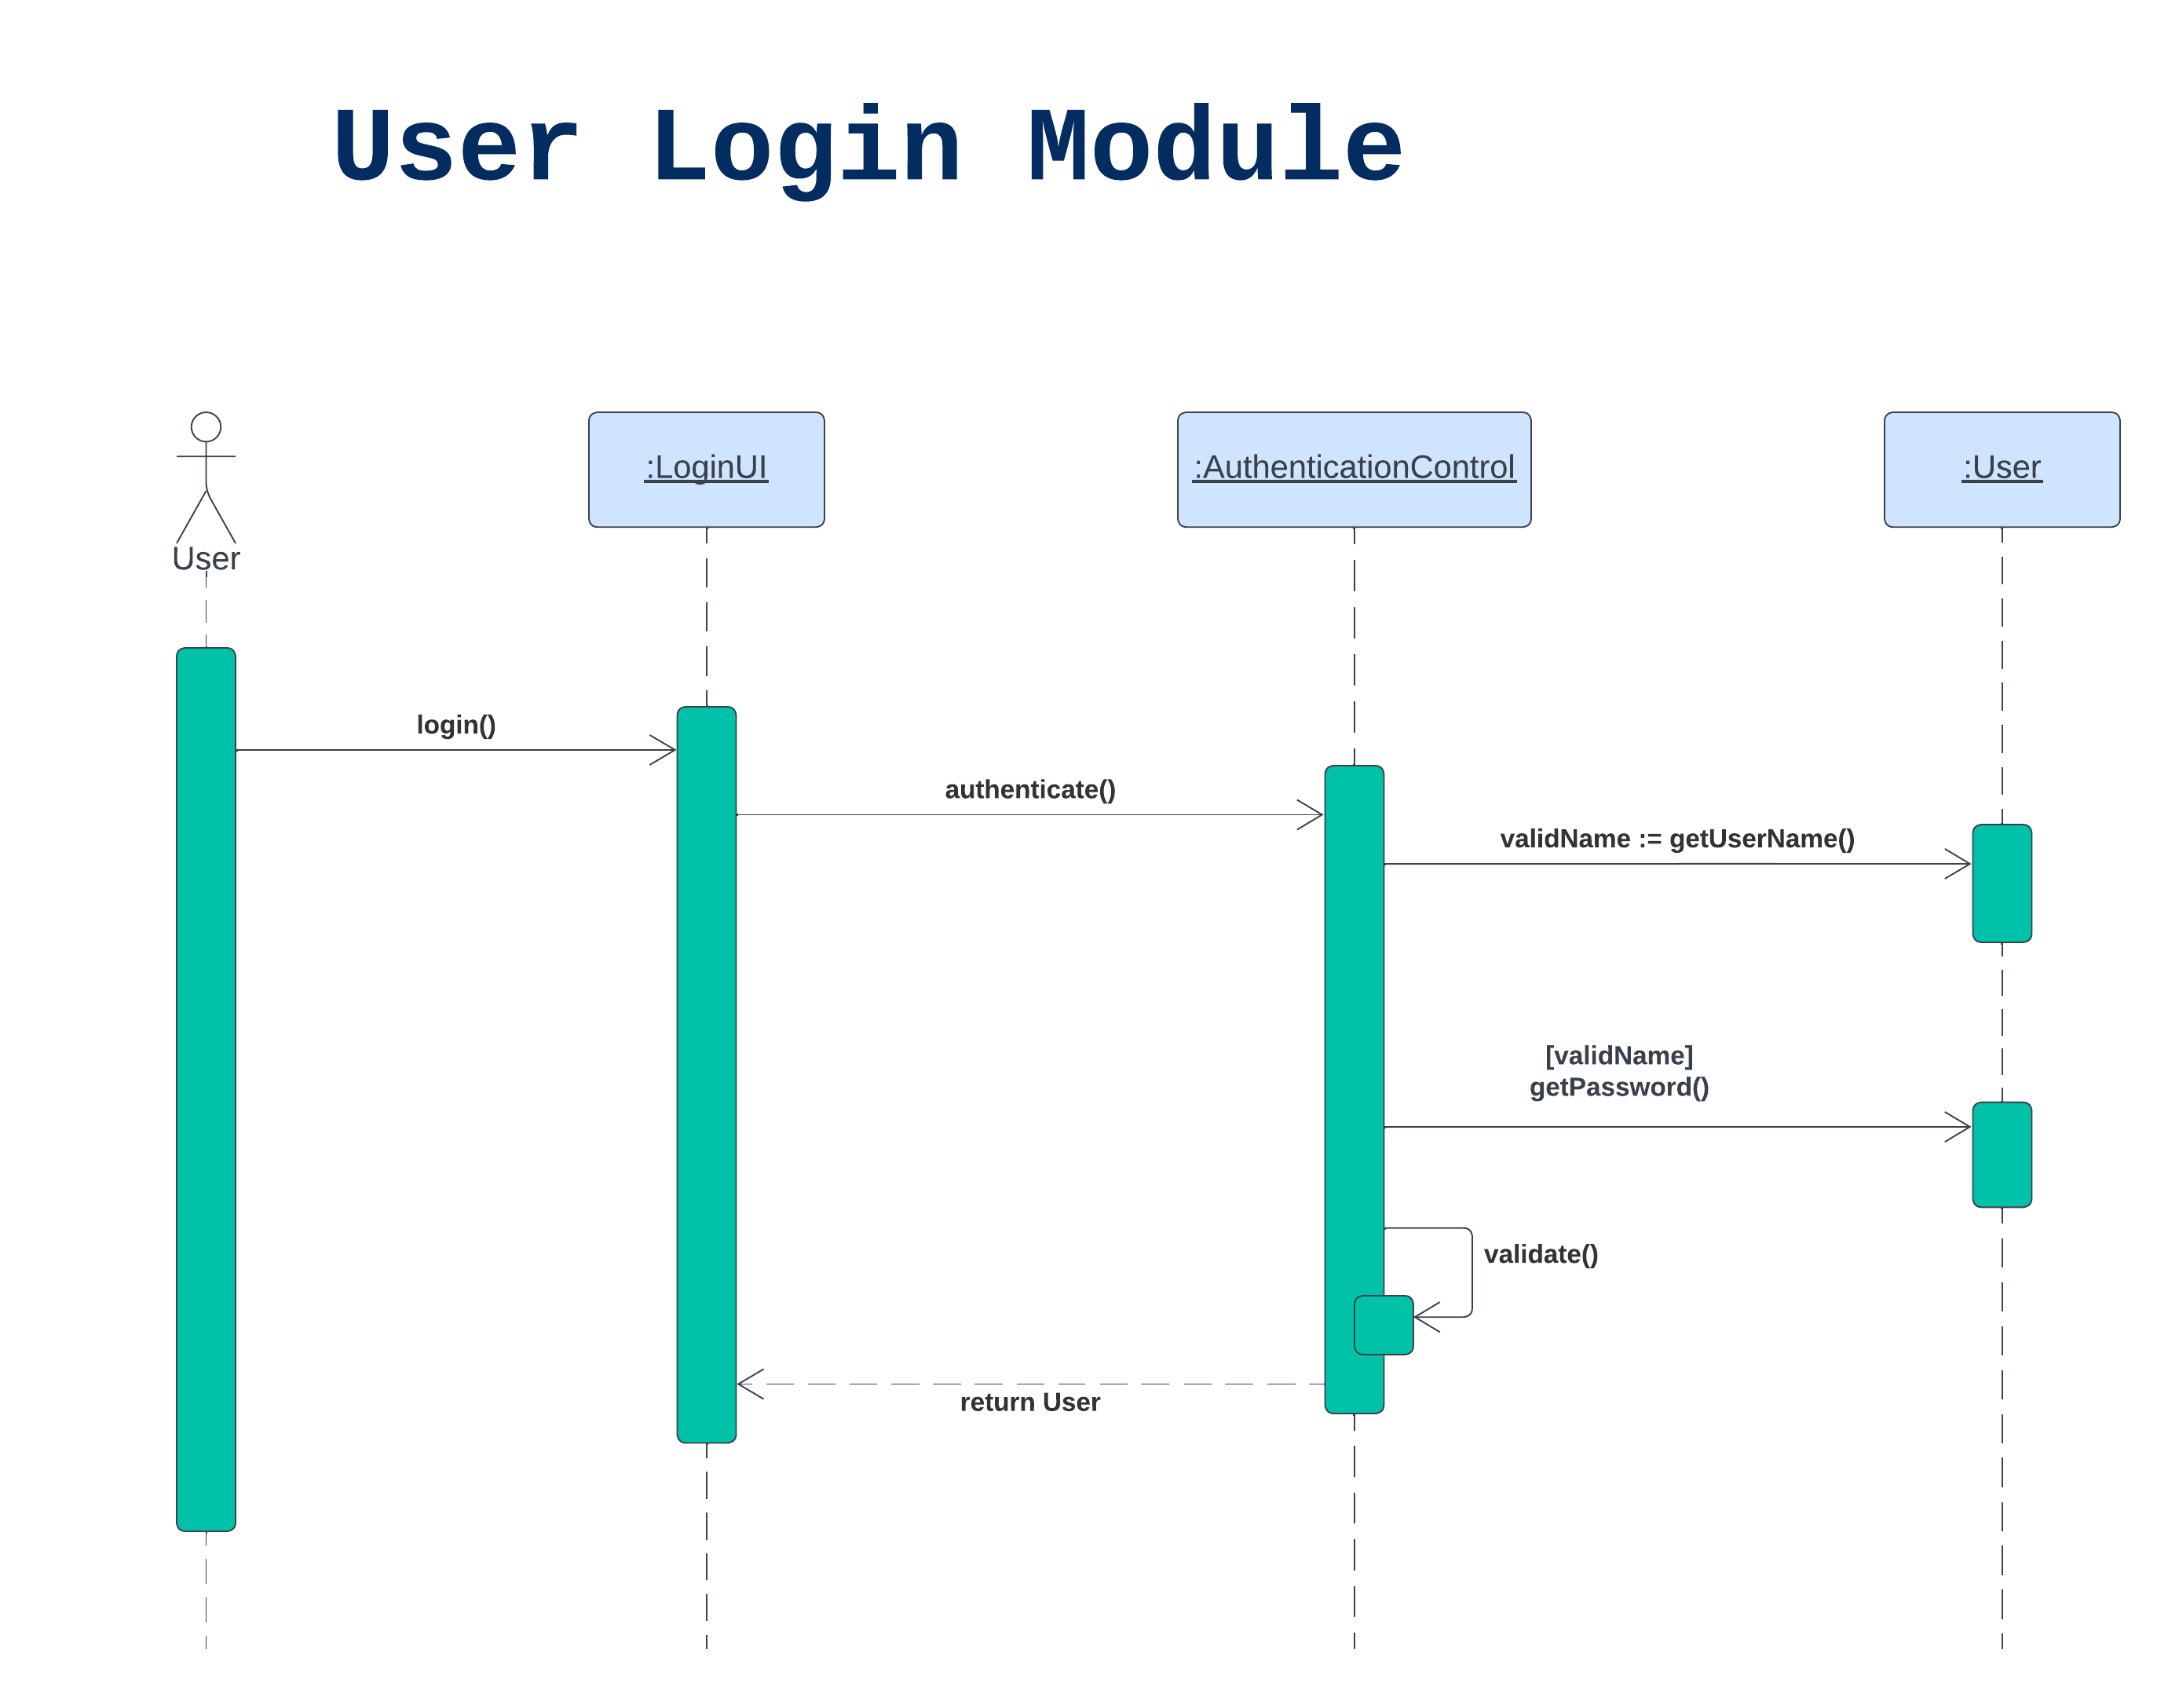
\includegraphics[width=0.78\textwidth]{Sequence Diagram/Login.png}
        \label{fig:SeqLogin}
    \caption{Sequence Diagram - User Login}
\end{figure}

\subsection{Profile Dashboard}
\begin{figure}[H]
    \centering
        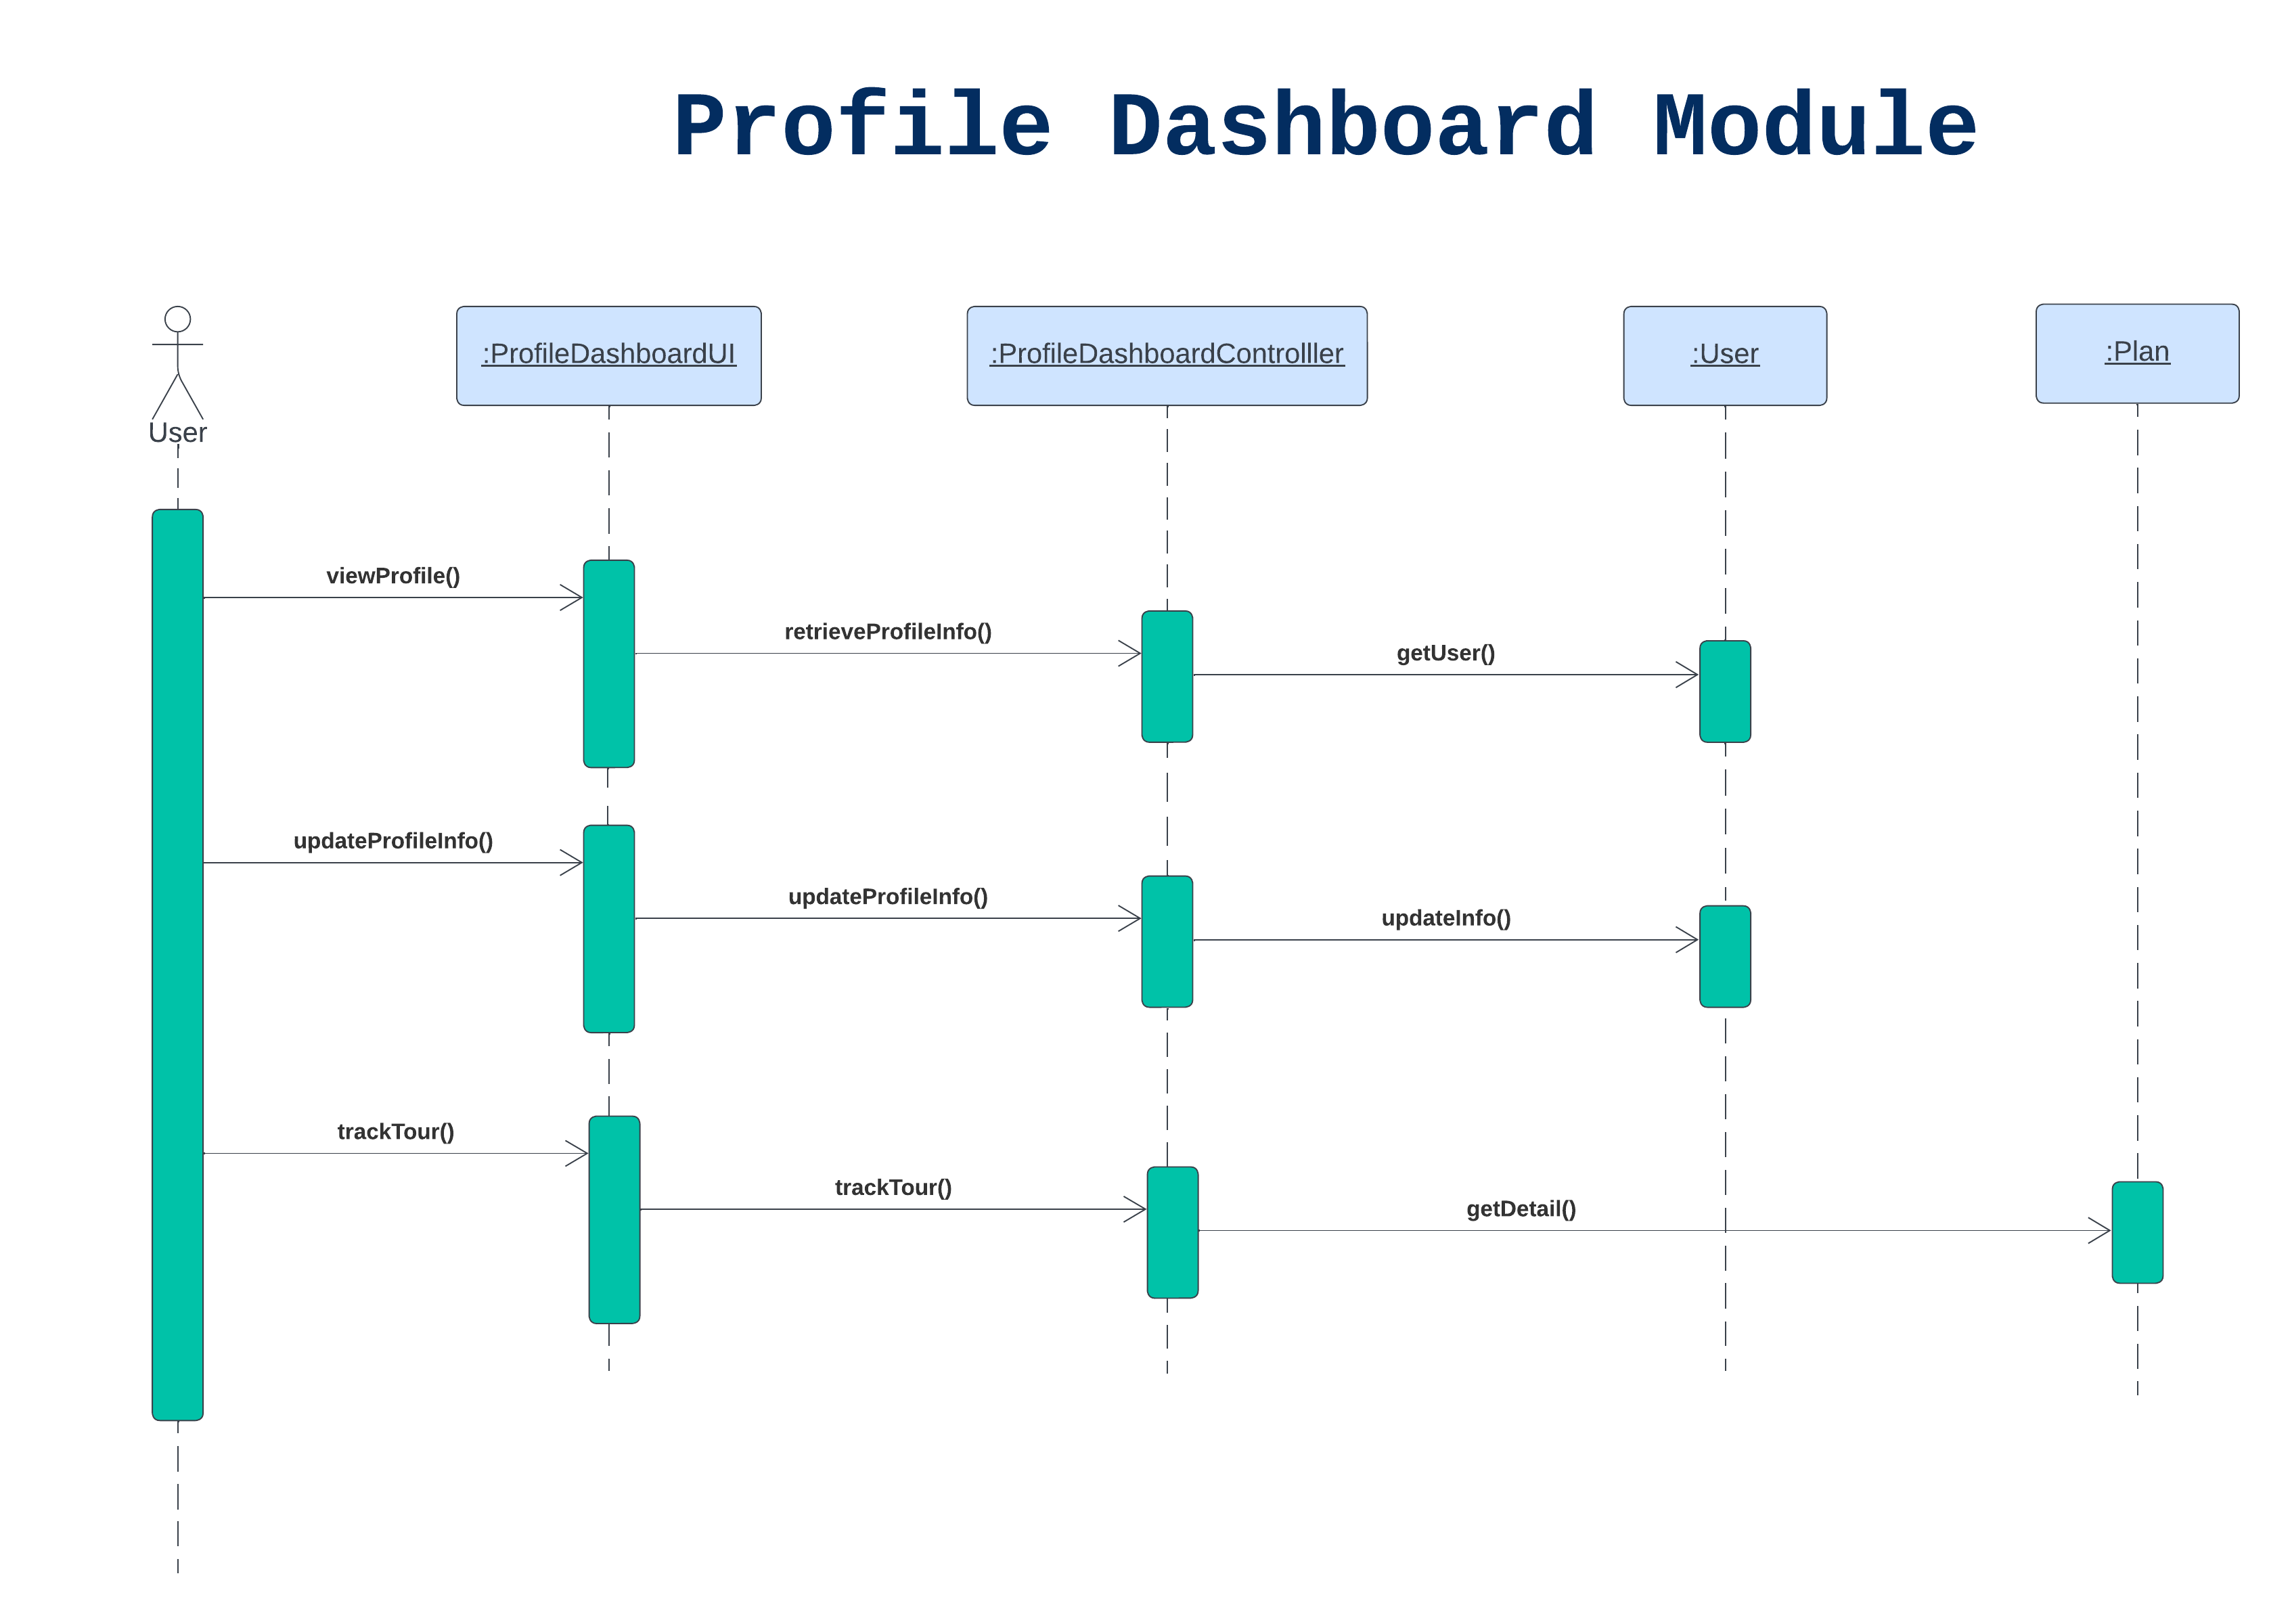
\includegraphics[width=0.78\textwidth]{Sequence Diagram/ProfileDashboard.png}
        \label{fig:SeqProfile}
    \caption{Sequence Diagram - Profile Dashboard}
\end{figure}

\newpage
\subsection{Destinations}
\begin{figure}[H]
    \centering
        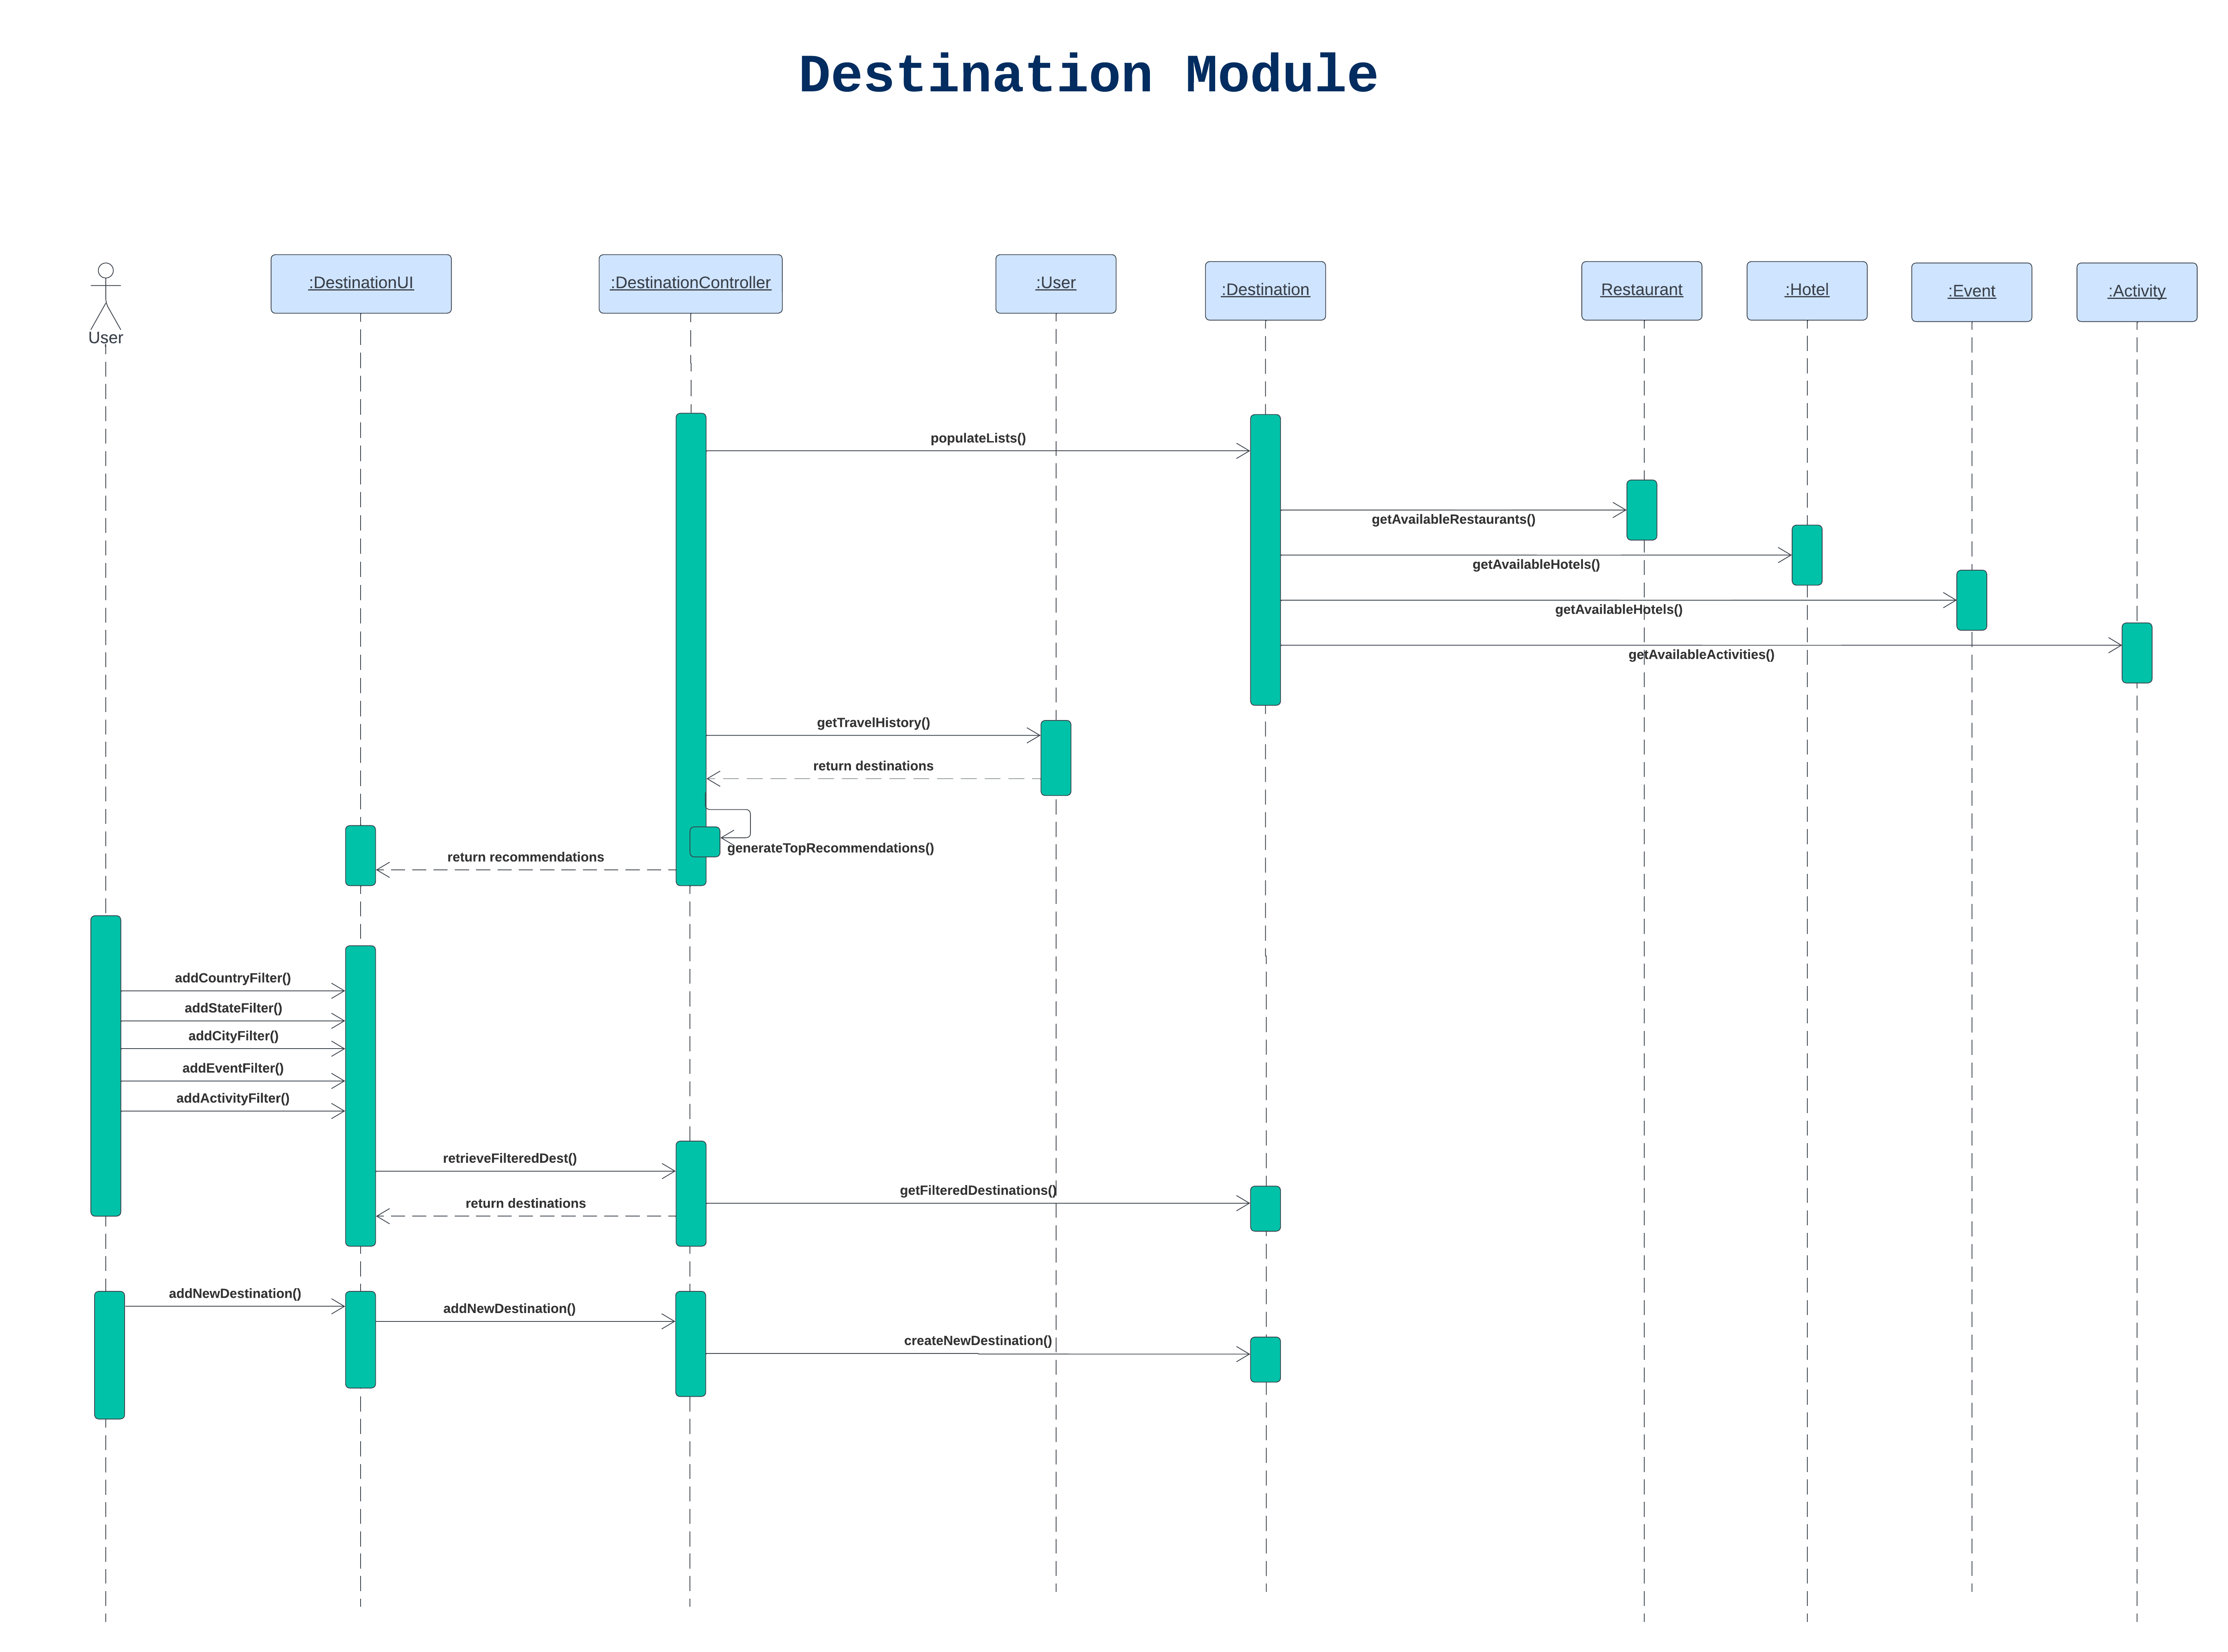
\includegraphics[width=0.80\textwidth]{Sequence Diagram/Destination.png}
        \label{fig:SeqDest}
    \caption{Sequence Diagram - Destinations}
\end{figure}

\subsection{Destination Details}
\begin{figure}[H]
    \centering
        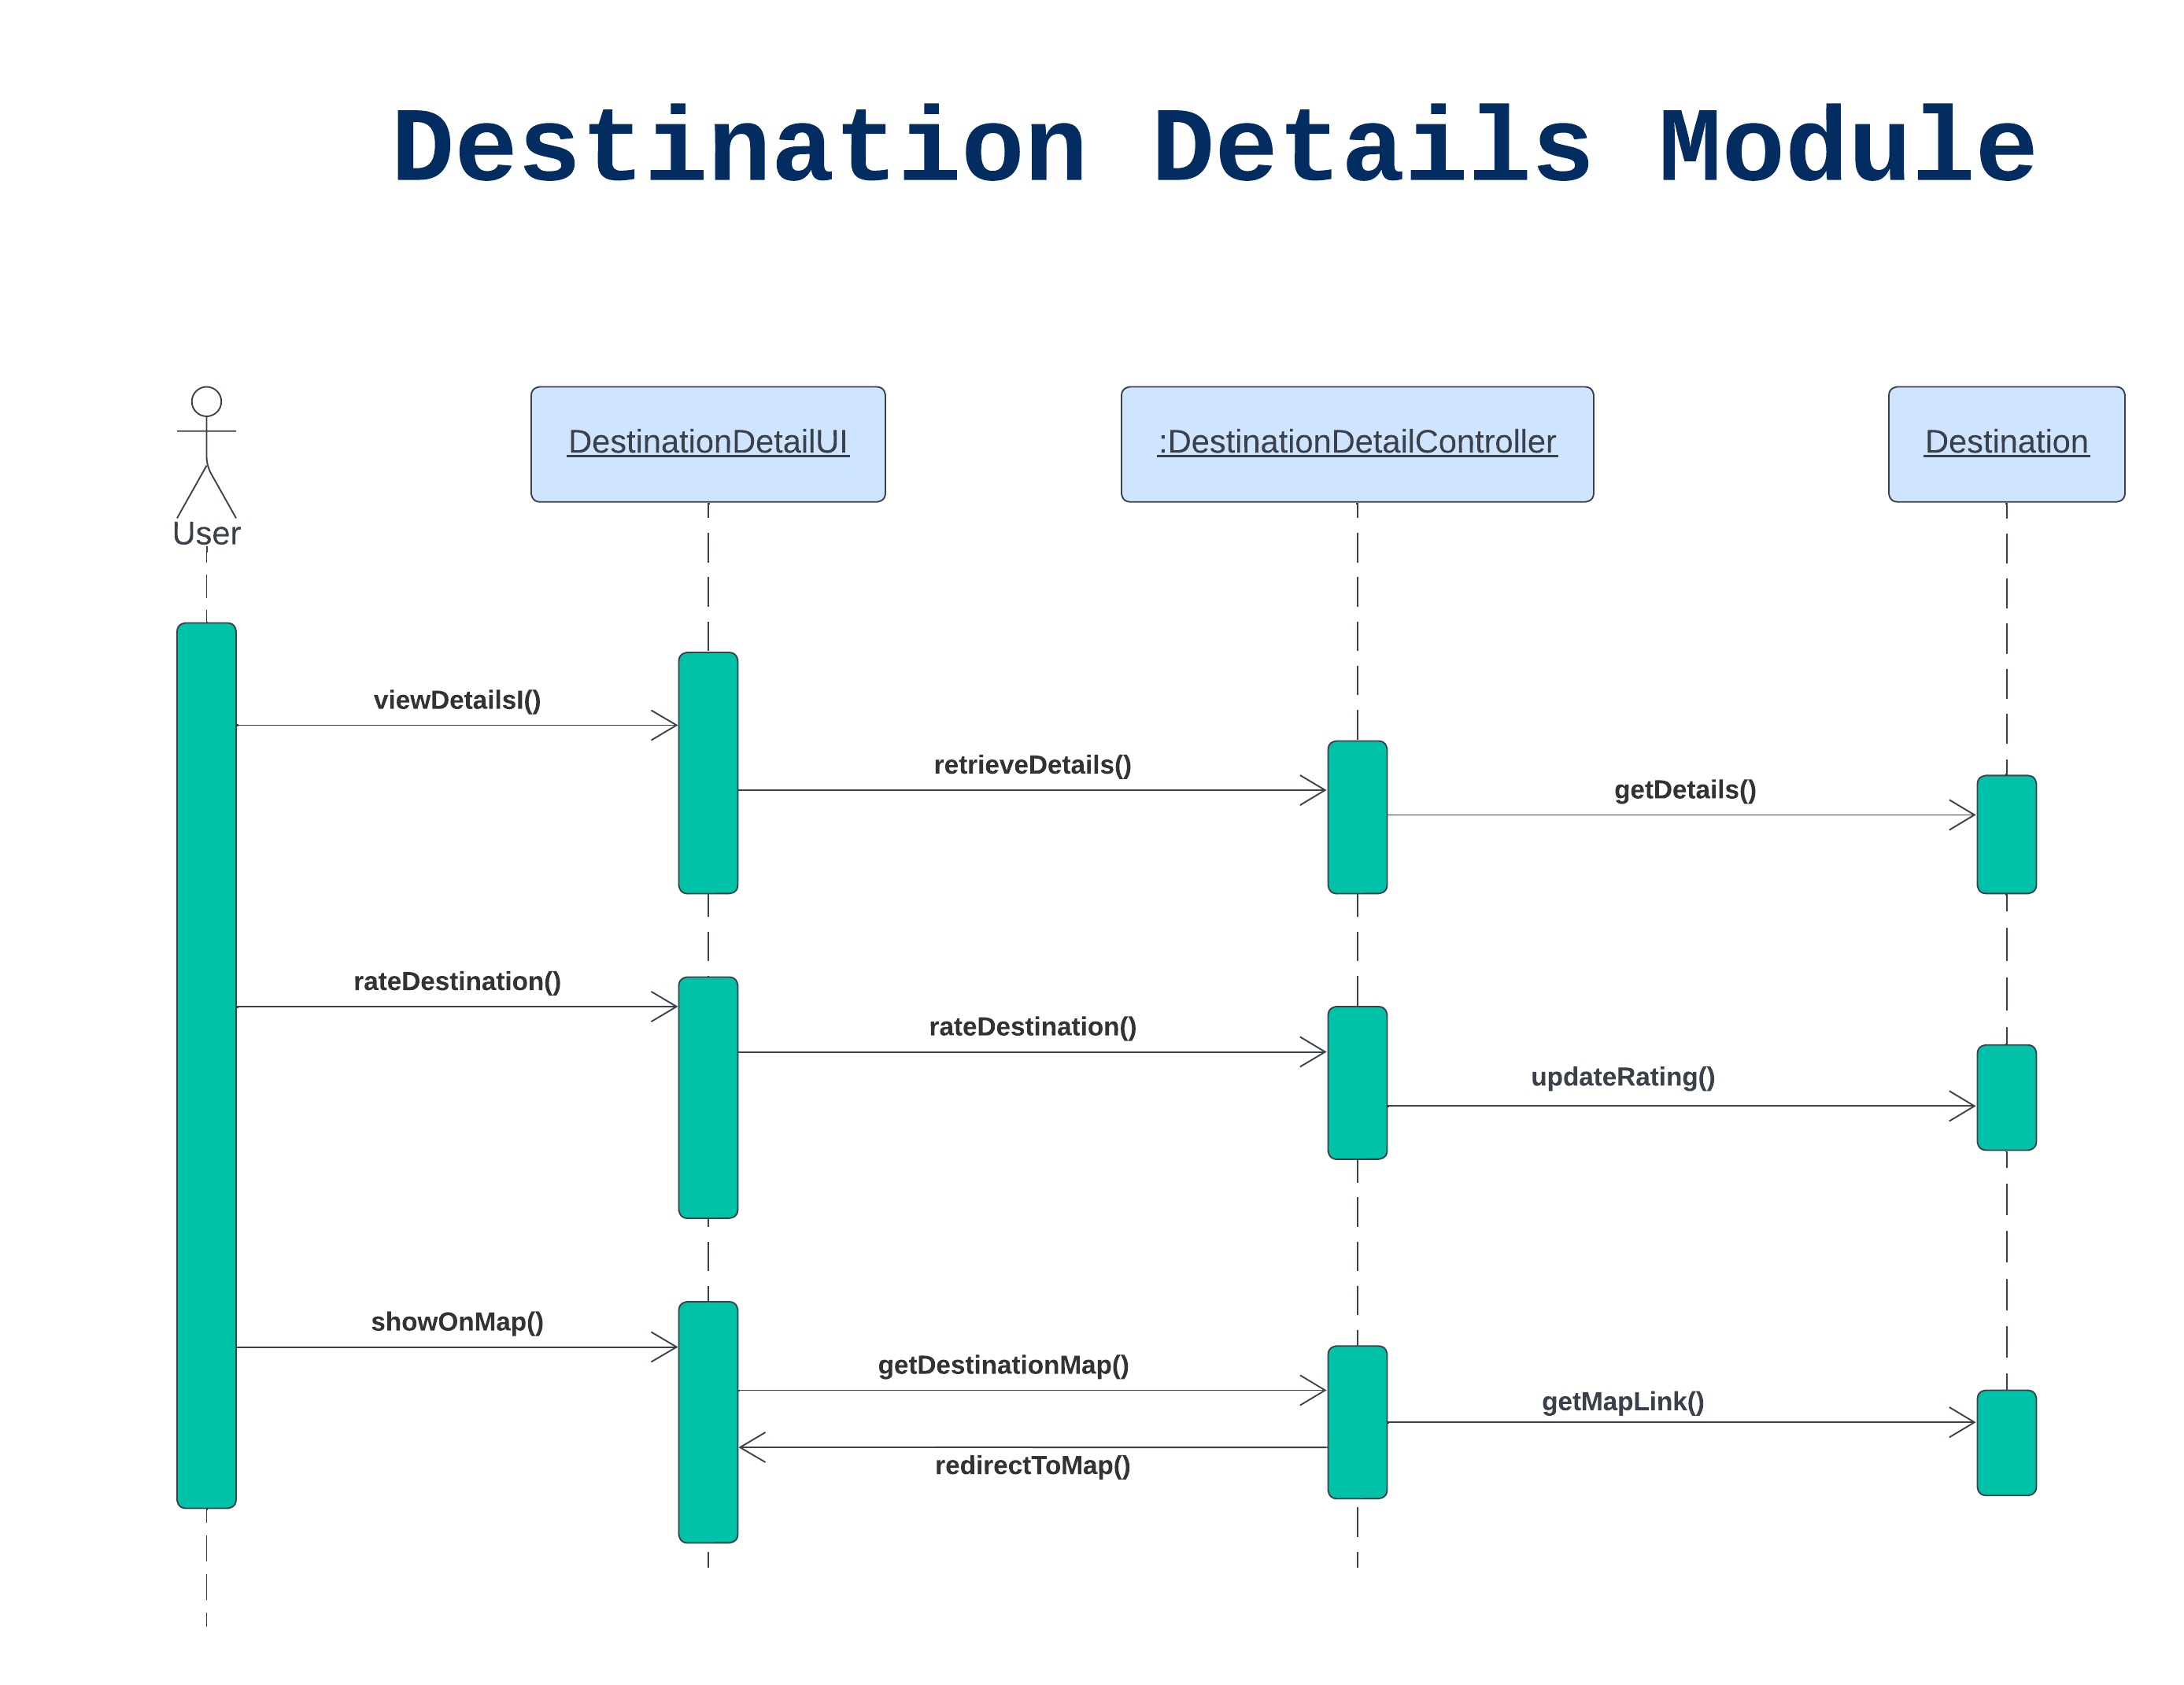
\includegraphics[width=0.75\textwidth]{Sequence Diagram/DestinationDetail.png}
        \label{fig:SeqDestDetails}
    \caption{Sequence Diagram - Destination Details}
\end{figure}

\newpage
\subsection{Plans}
\begin{figure}[H]
    \centering
        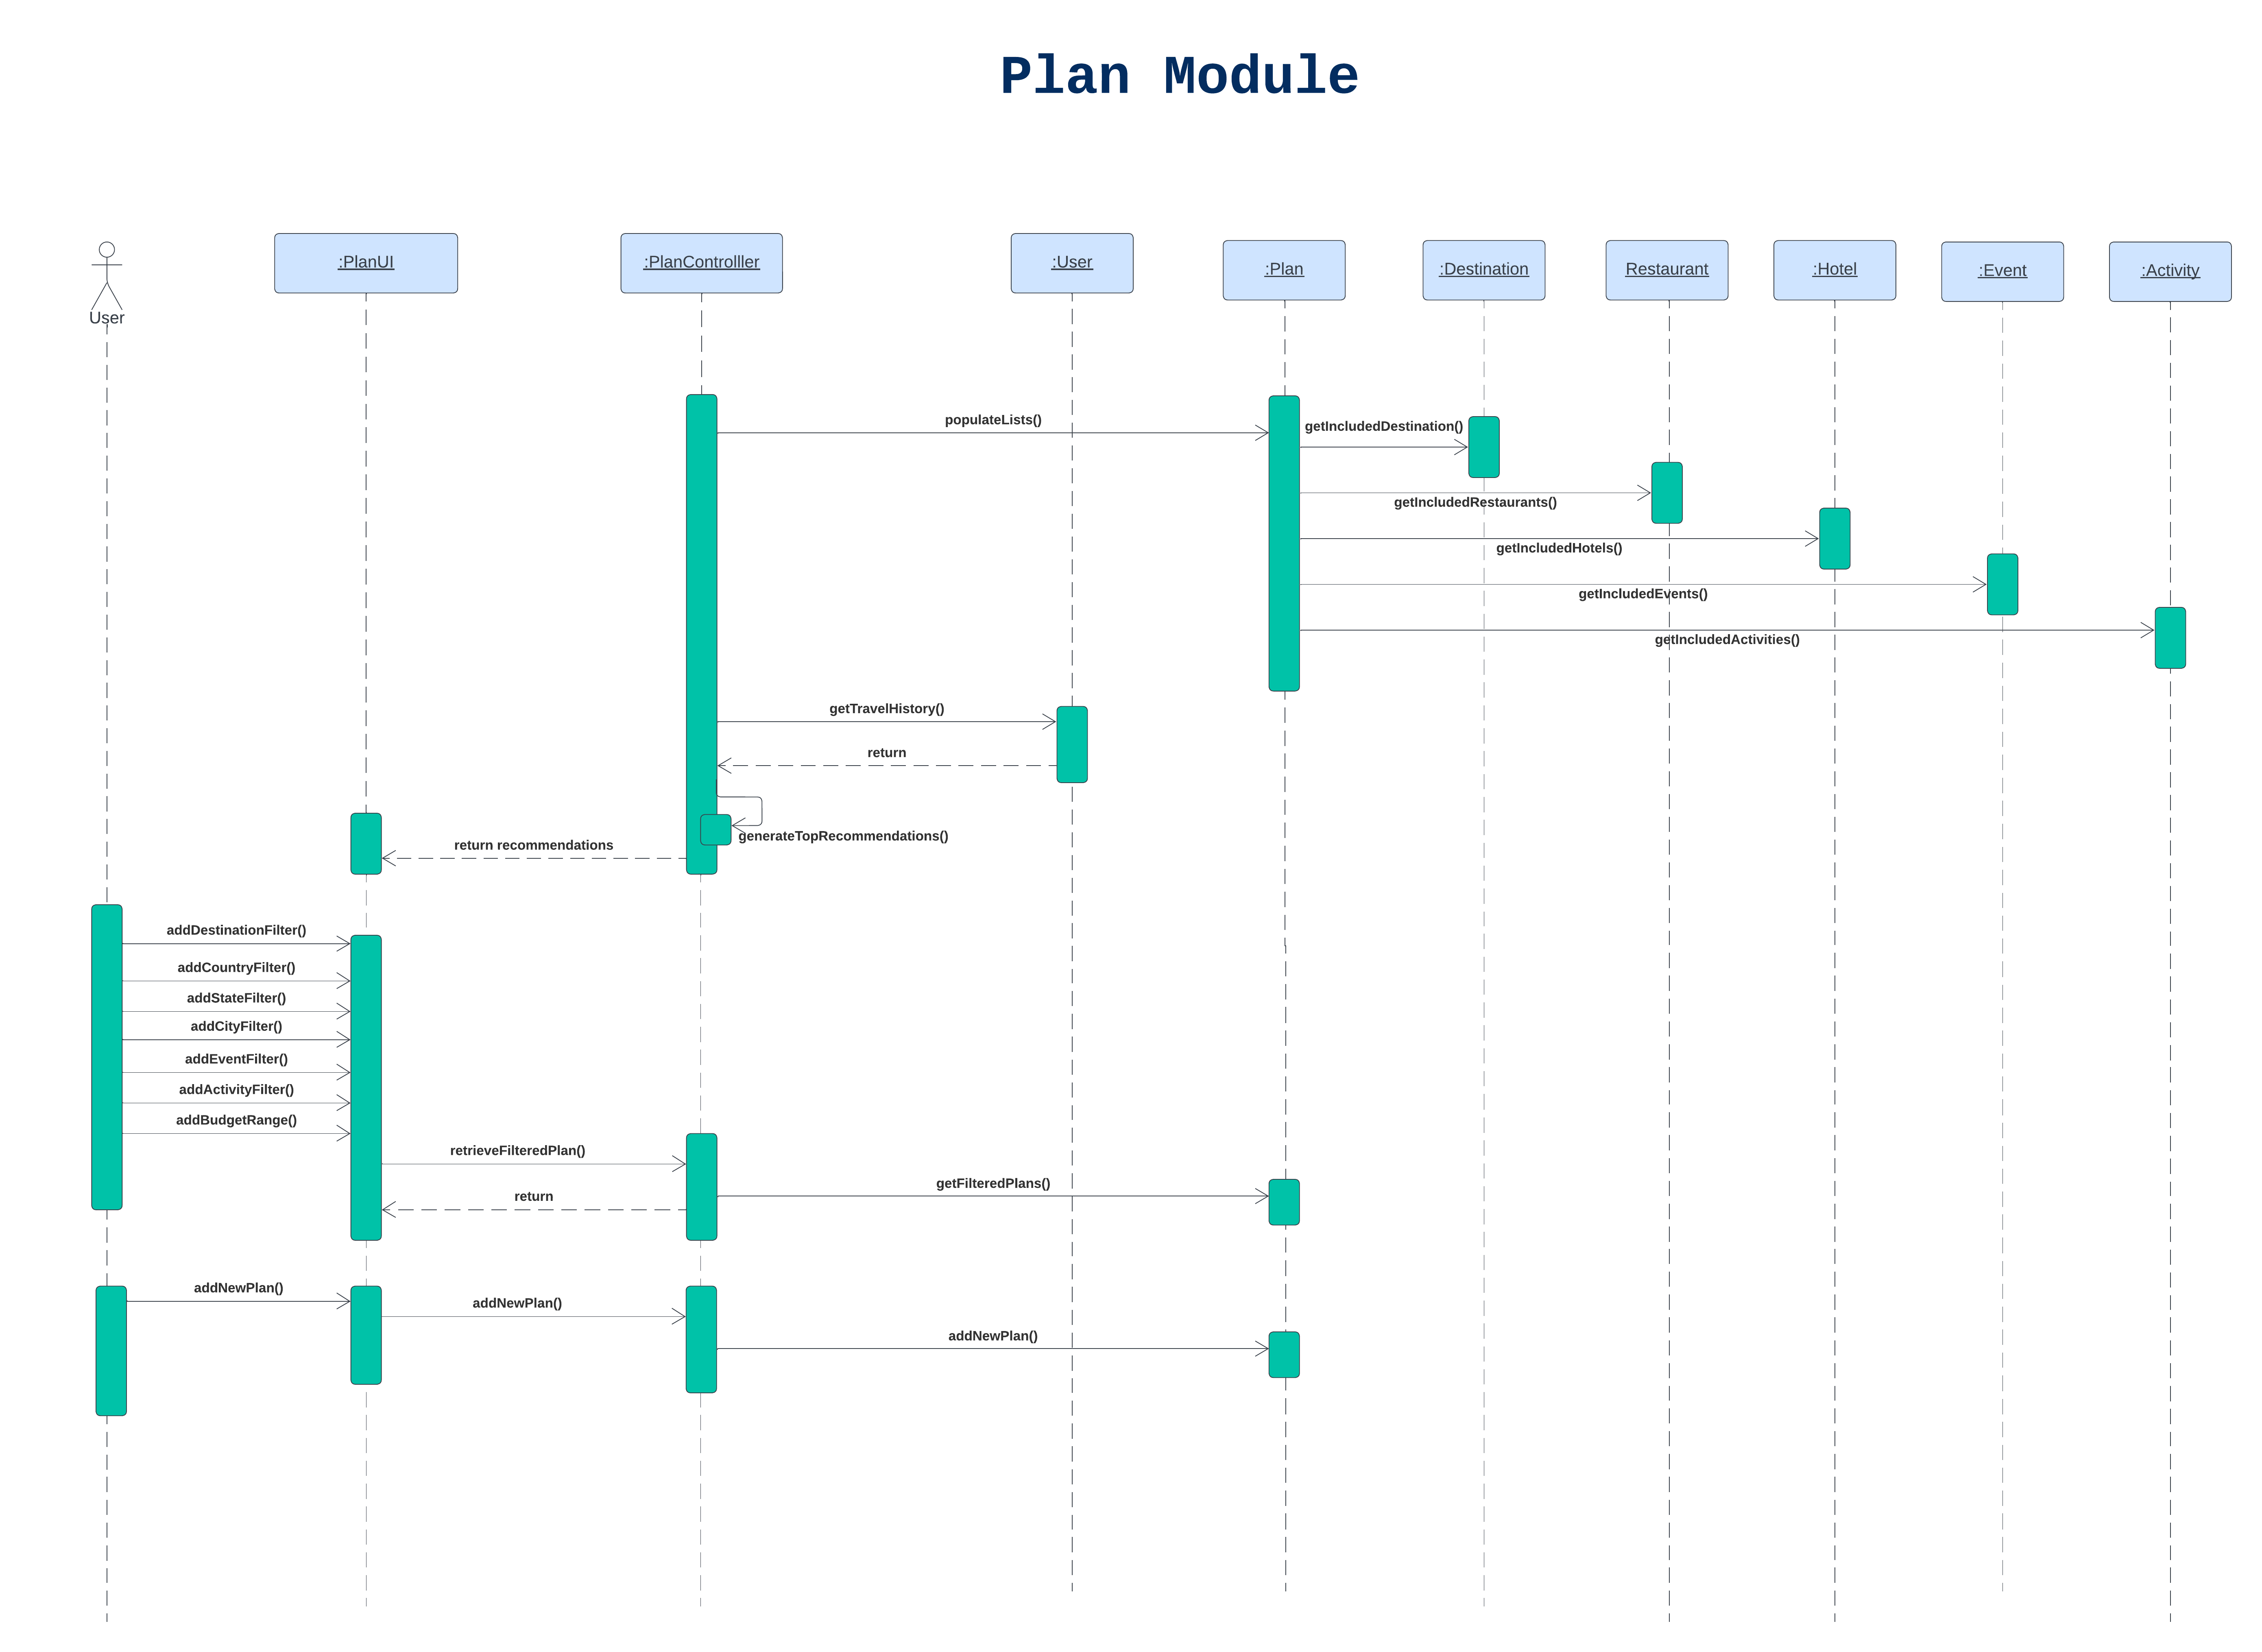
\includegraphics[width=0.75\textwidth]{Sequence Diagram/Plan.png}
        \label{fig:SeqPlans}
    \caption{Sequence Diagram - Plans}
\end{figure}

\subsection{Plan Details}
\begin{figure}[H]
    \centering
        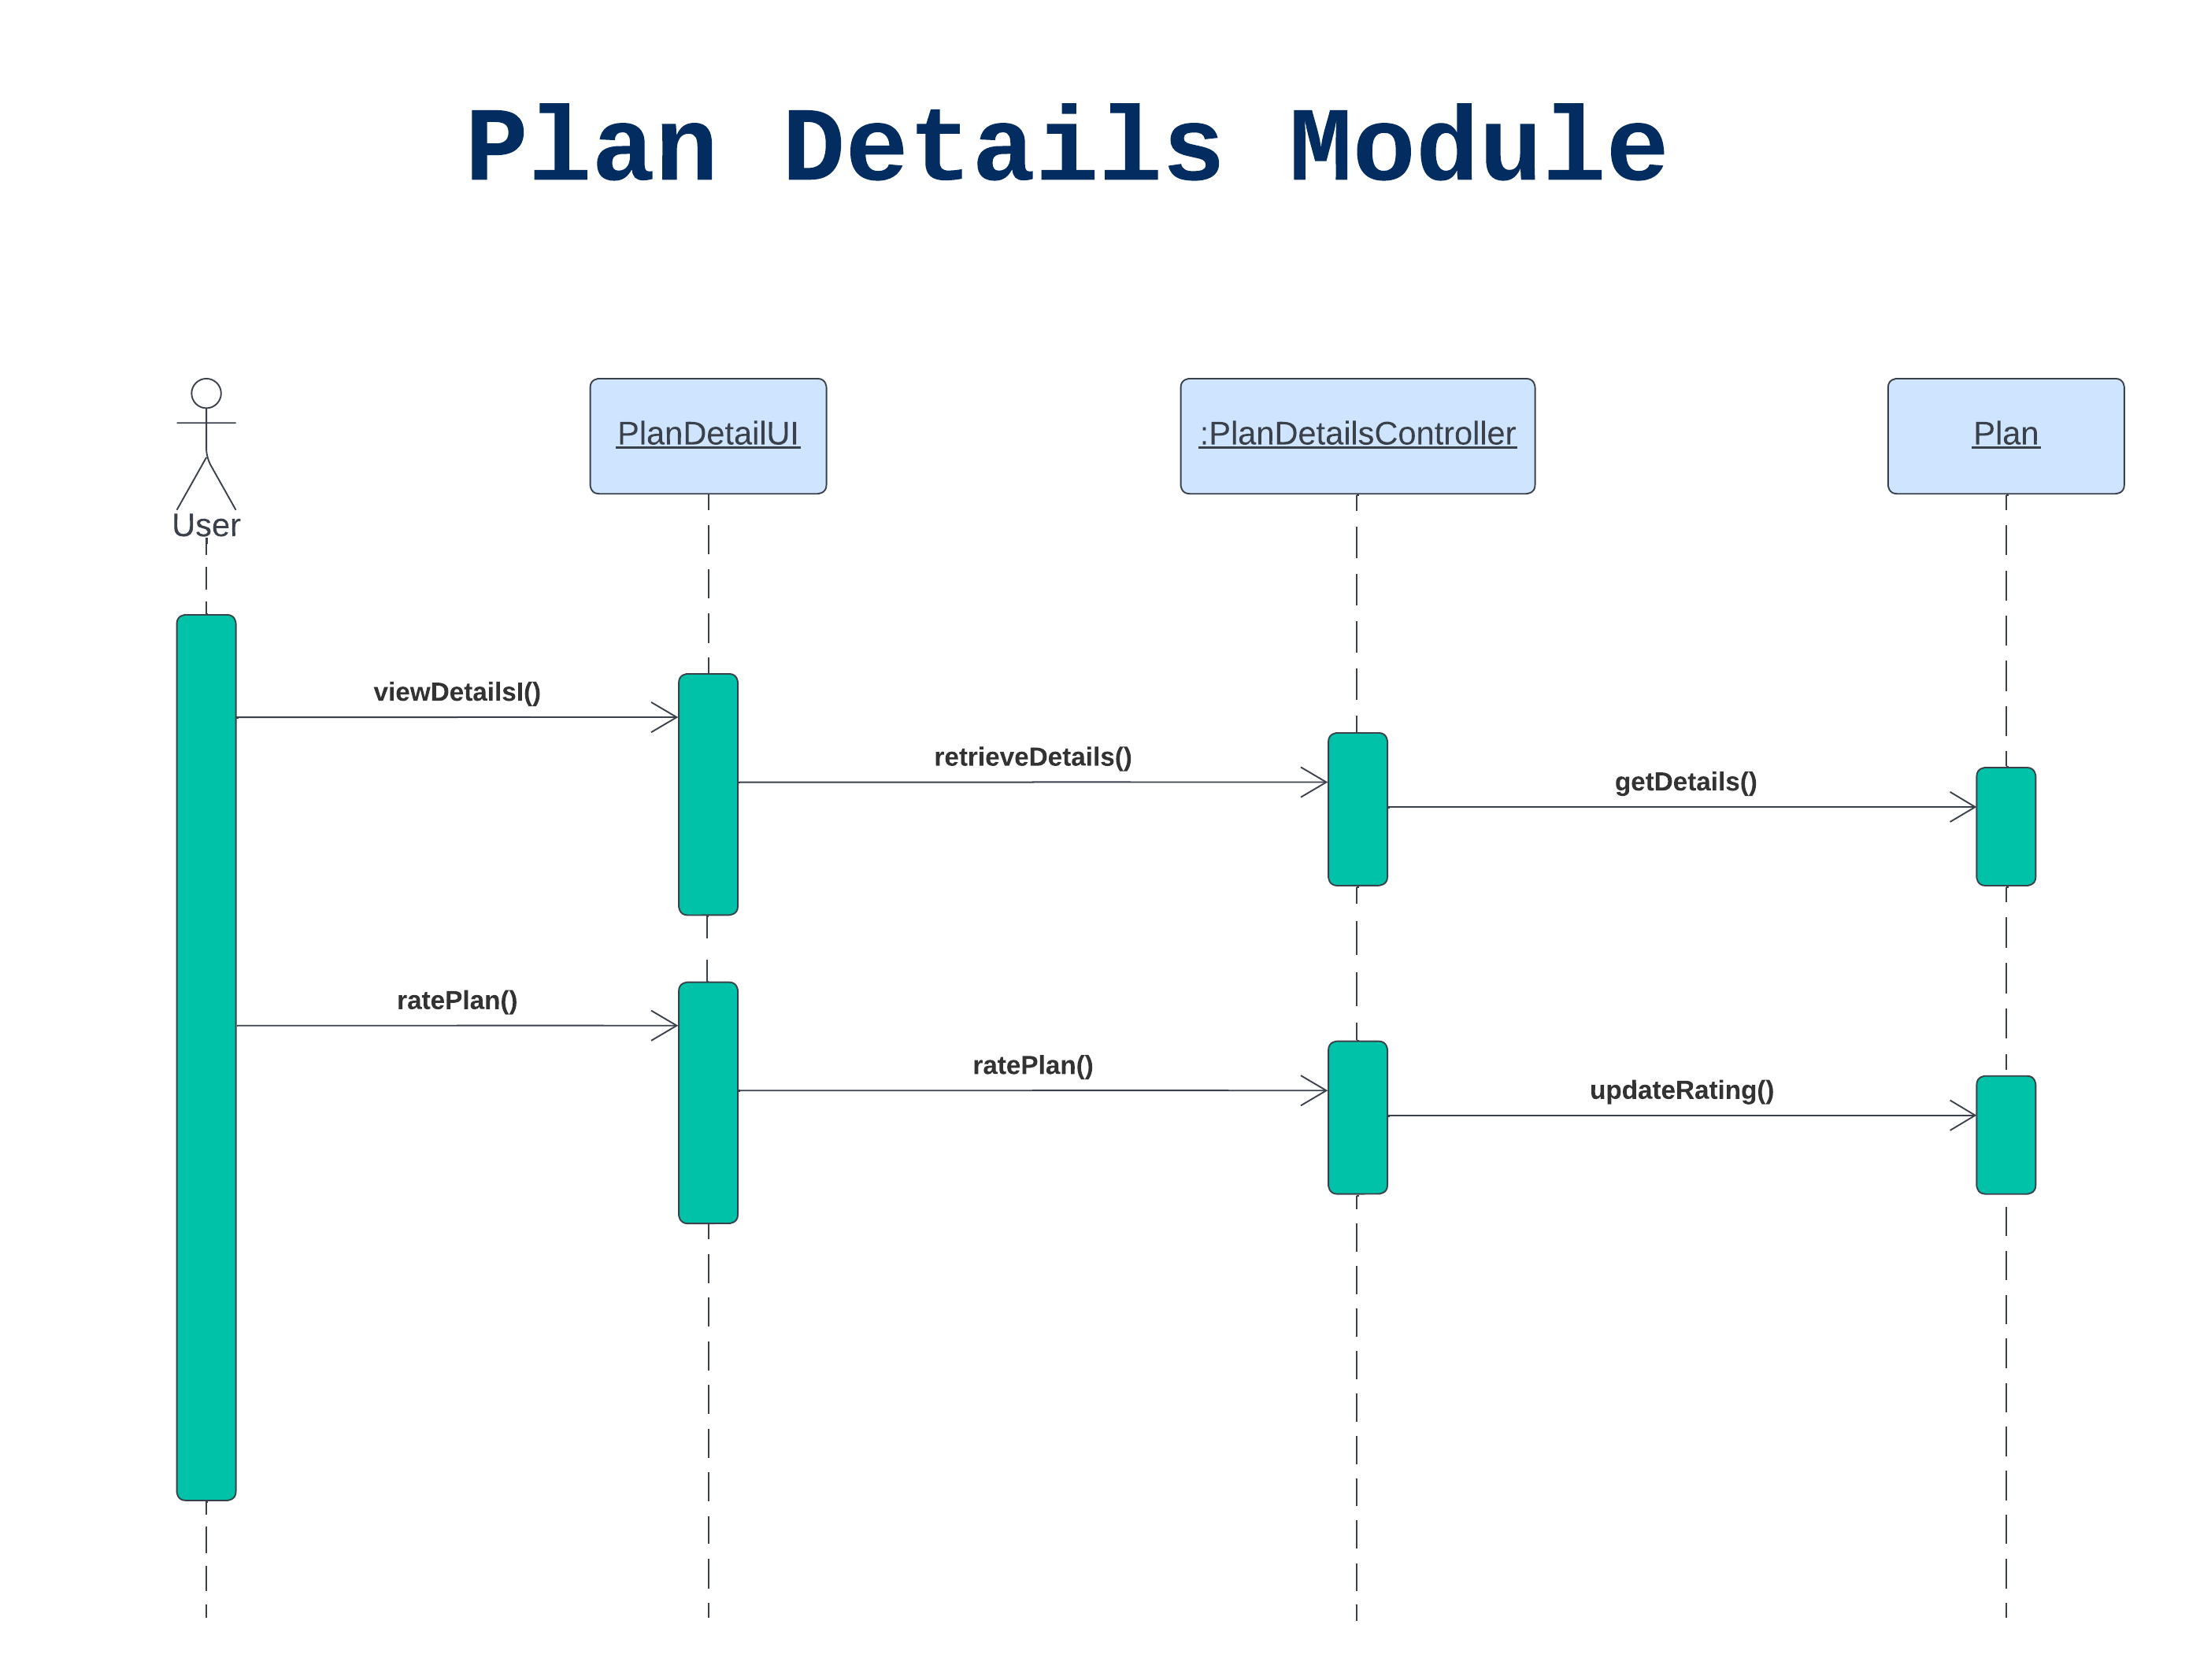
\includegraphics[width=0.75\textwidth]{Sequence Diagram/PlanDetails.png}
        \label{fig:SeqPlanDetails}
    \caption{Sequence Diagram - Plan Details}
\end{figure}

\newpage
\subsection{Customize Plans}
\begin{figure}[H]
    \centering
        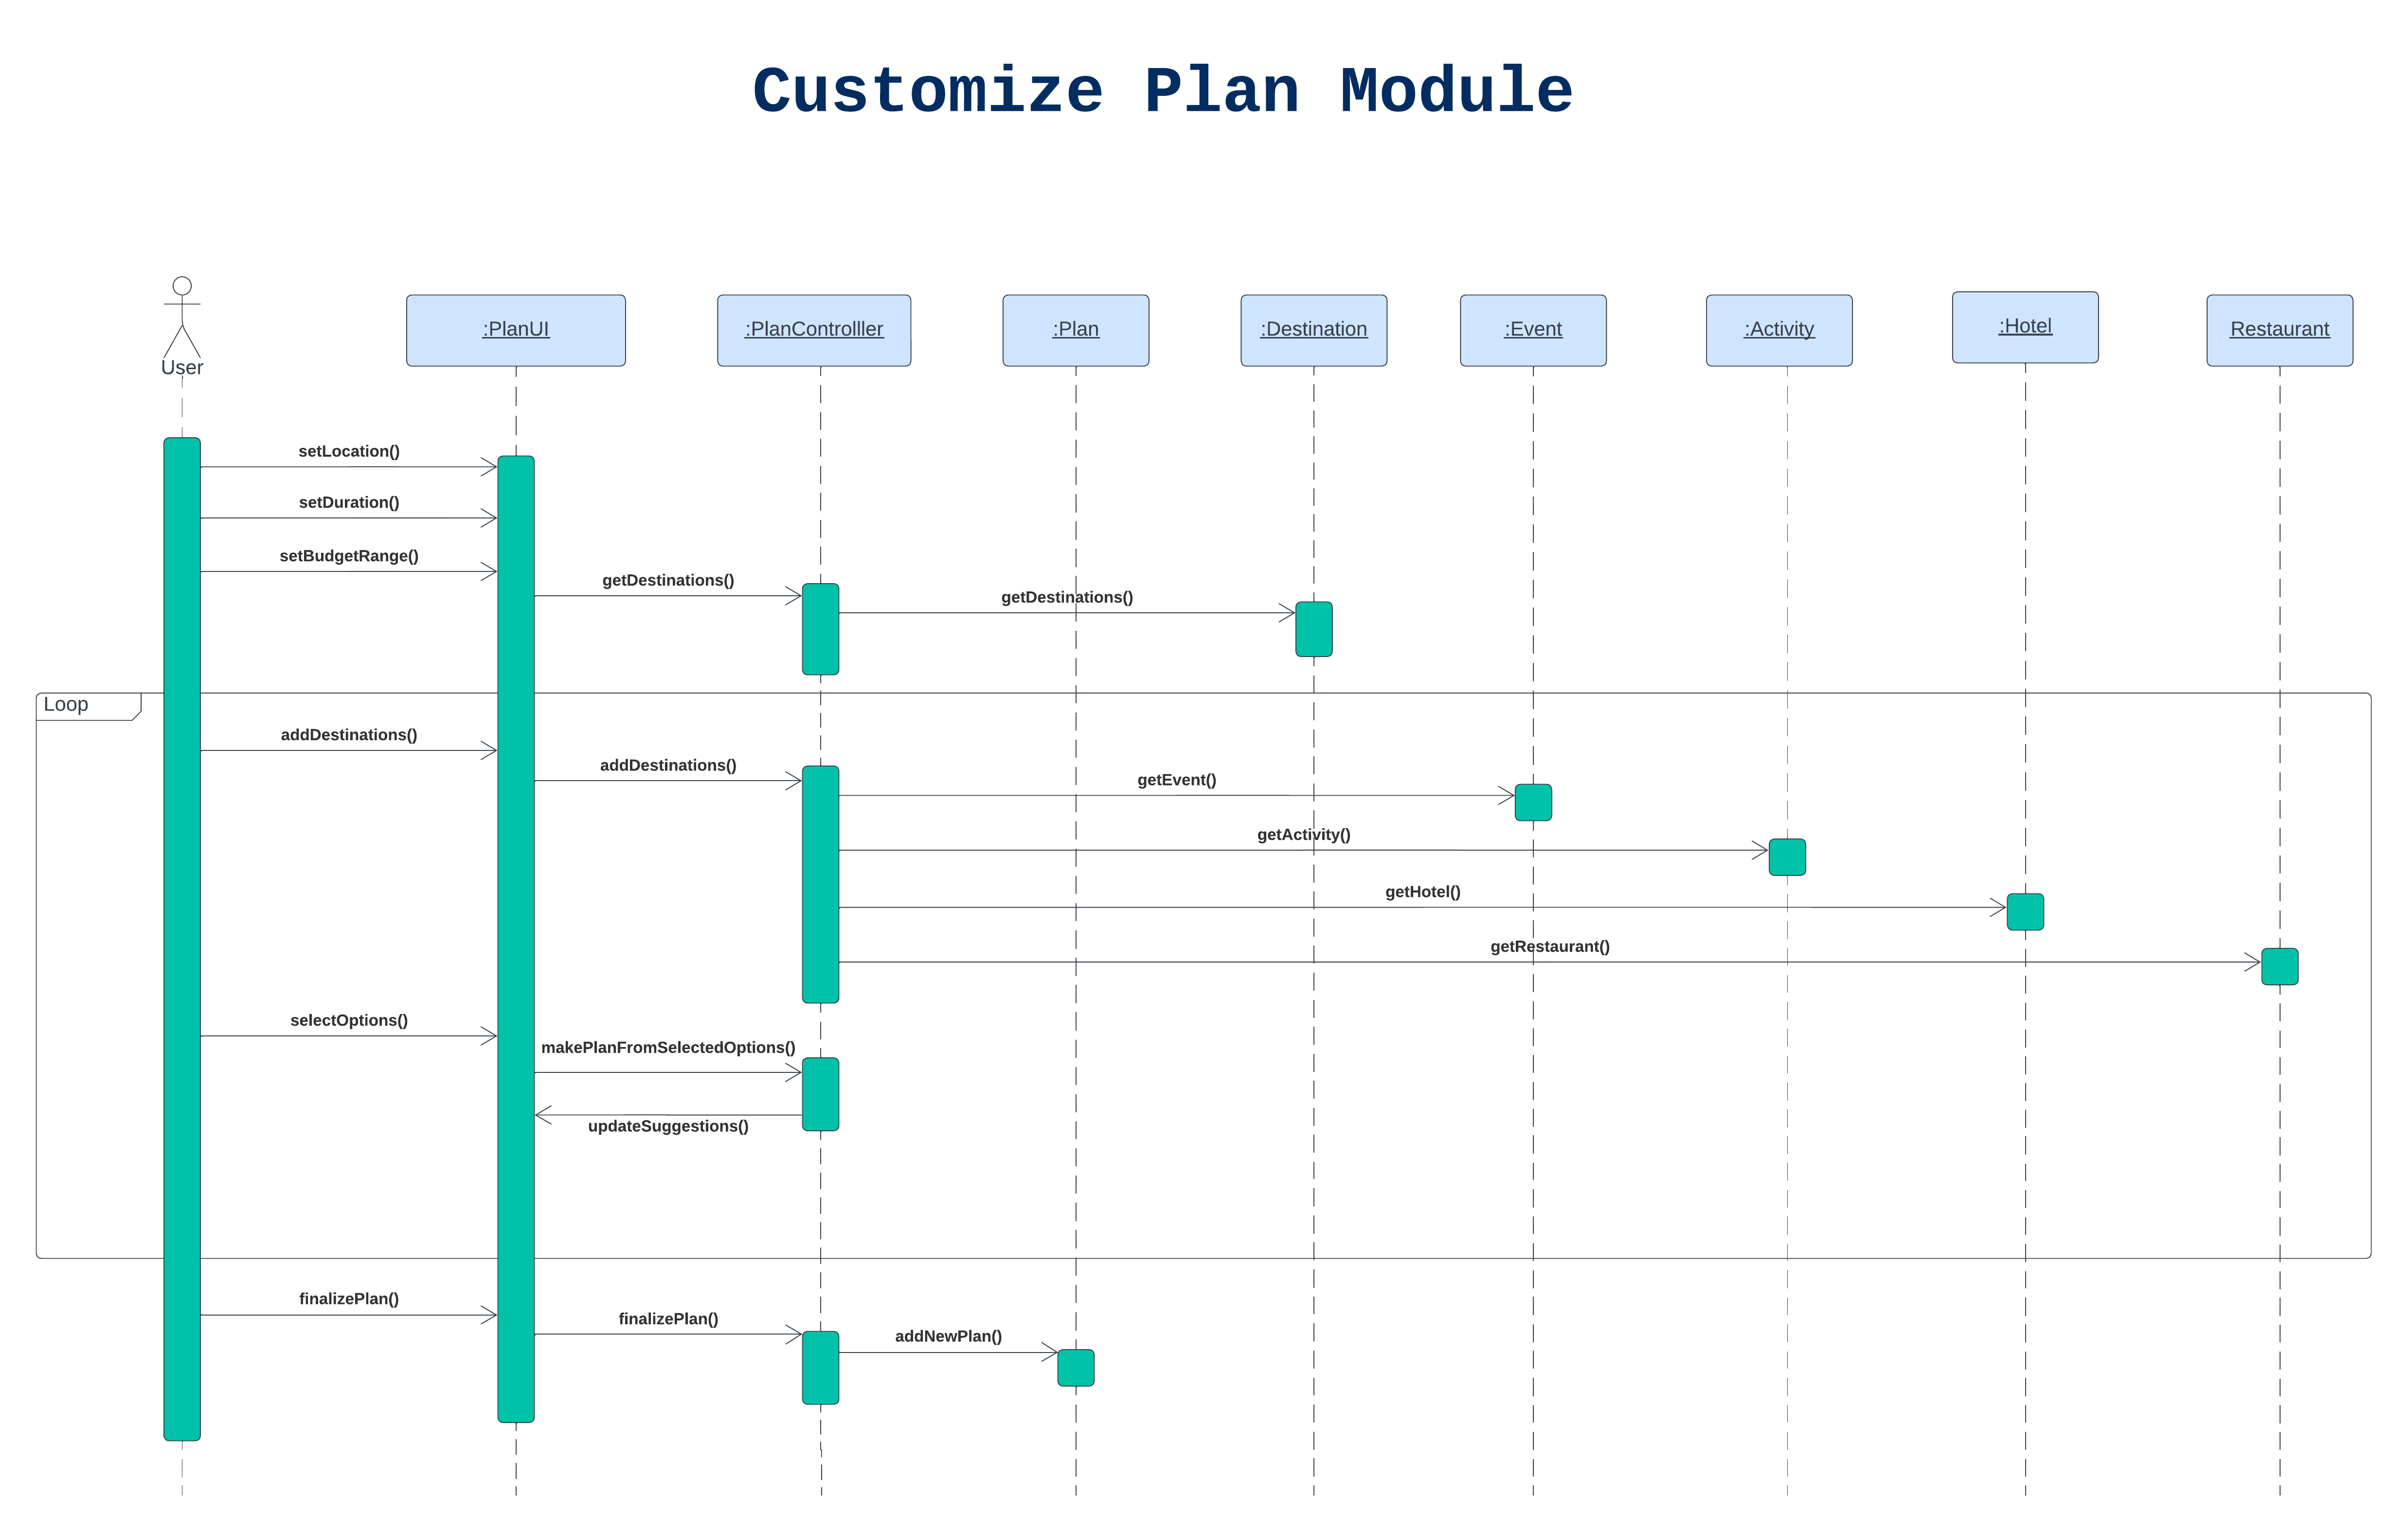
\includegraphics[width=0.75\textwidth]{Sequence Diagram/CustomizePlan.png}
        \label{fig:SeqCustPlan}
    \caption{Sequence Diagram - Customize Plans}
\end{figure}

\subsection{Tours}
\begin{figure}[H]
    \centering
        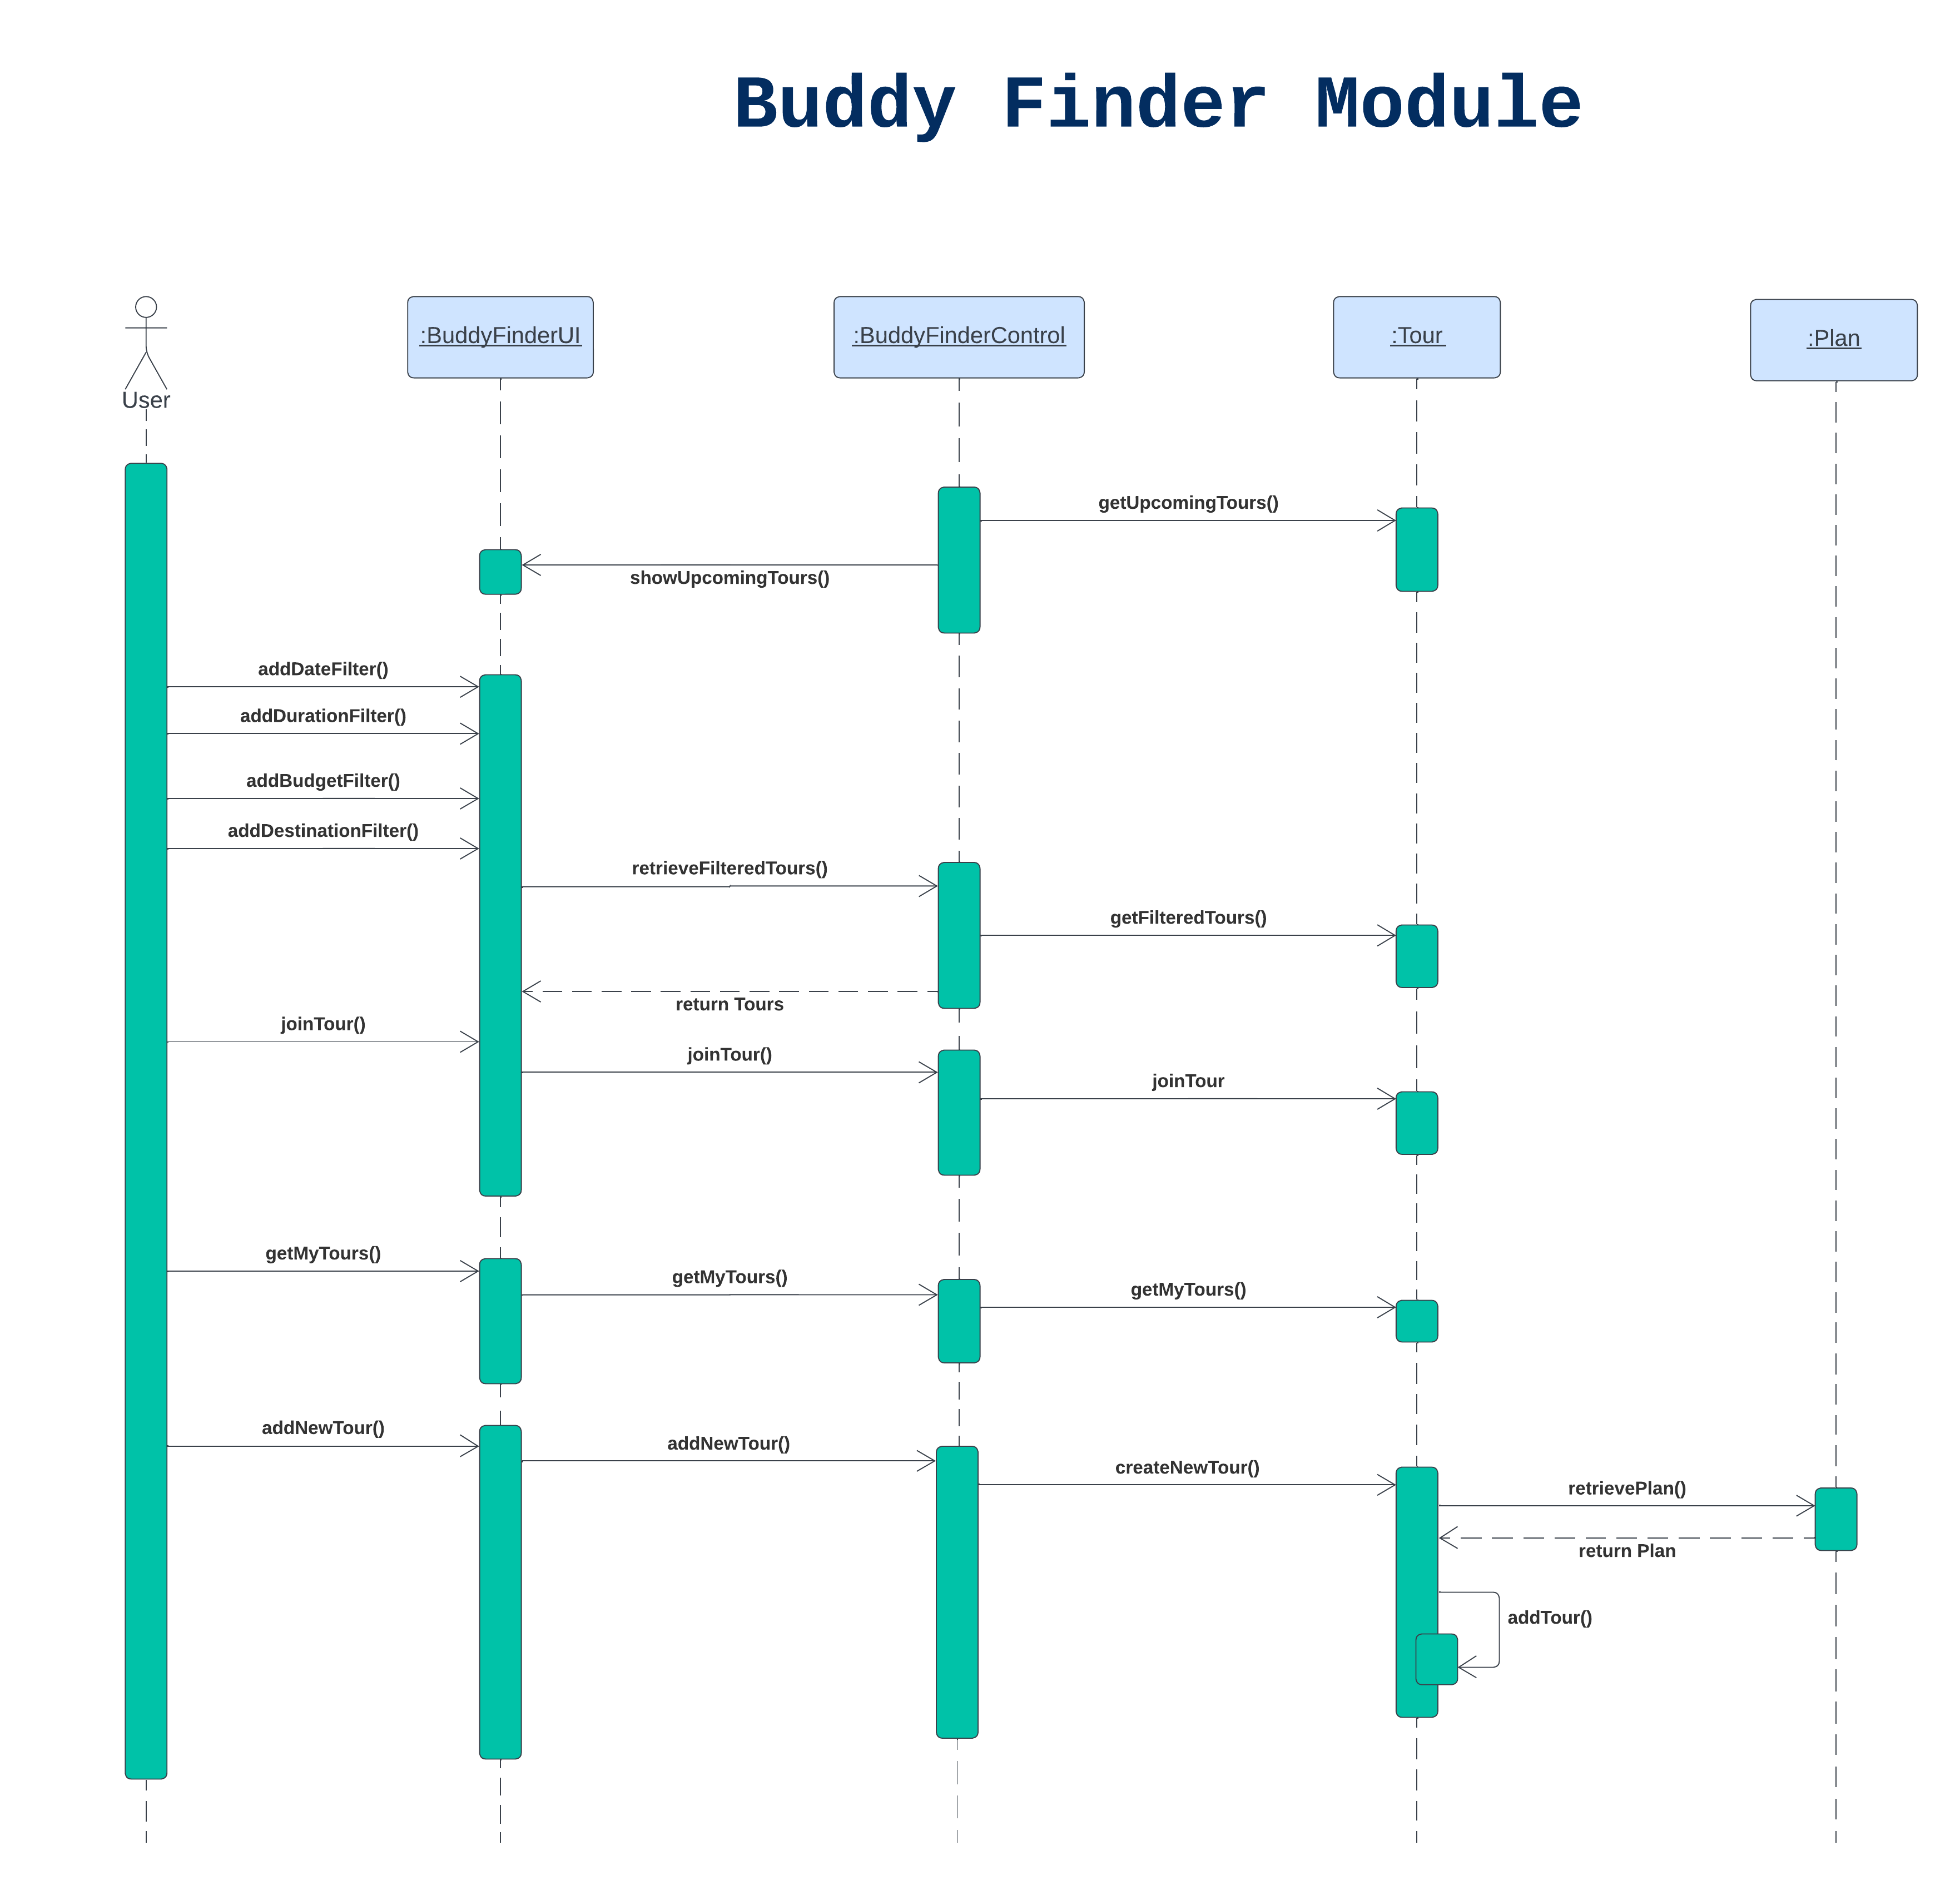
\includegraphics[width=0.70\textwidth]{Sequence Diagram/BuddyFinder.png}
        \label{fig:SeqTours}
    \caption{Sequence Diagram - Tours}
\end{figure}

\newpage

\section{Collaboration Diagrams}
\subsection{Feedbacks Acknowledged}

\begin{itemize}
    \item 'Actor' is replaced with the name of actor (i.e. User) 
\end{itemize}

\subsection{User Authentication}
\begin{figure}[H]
    \centering
        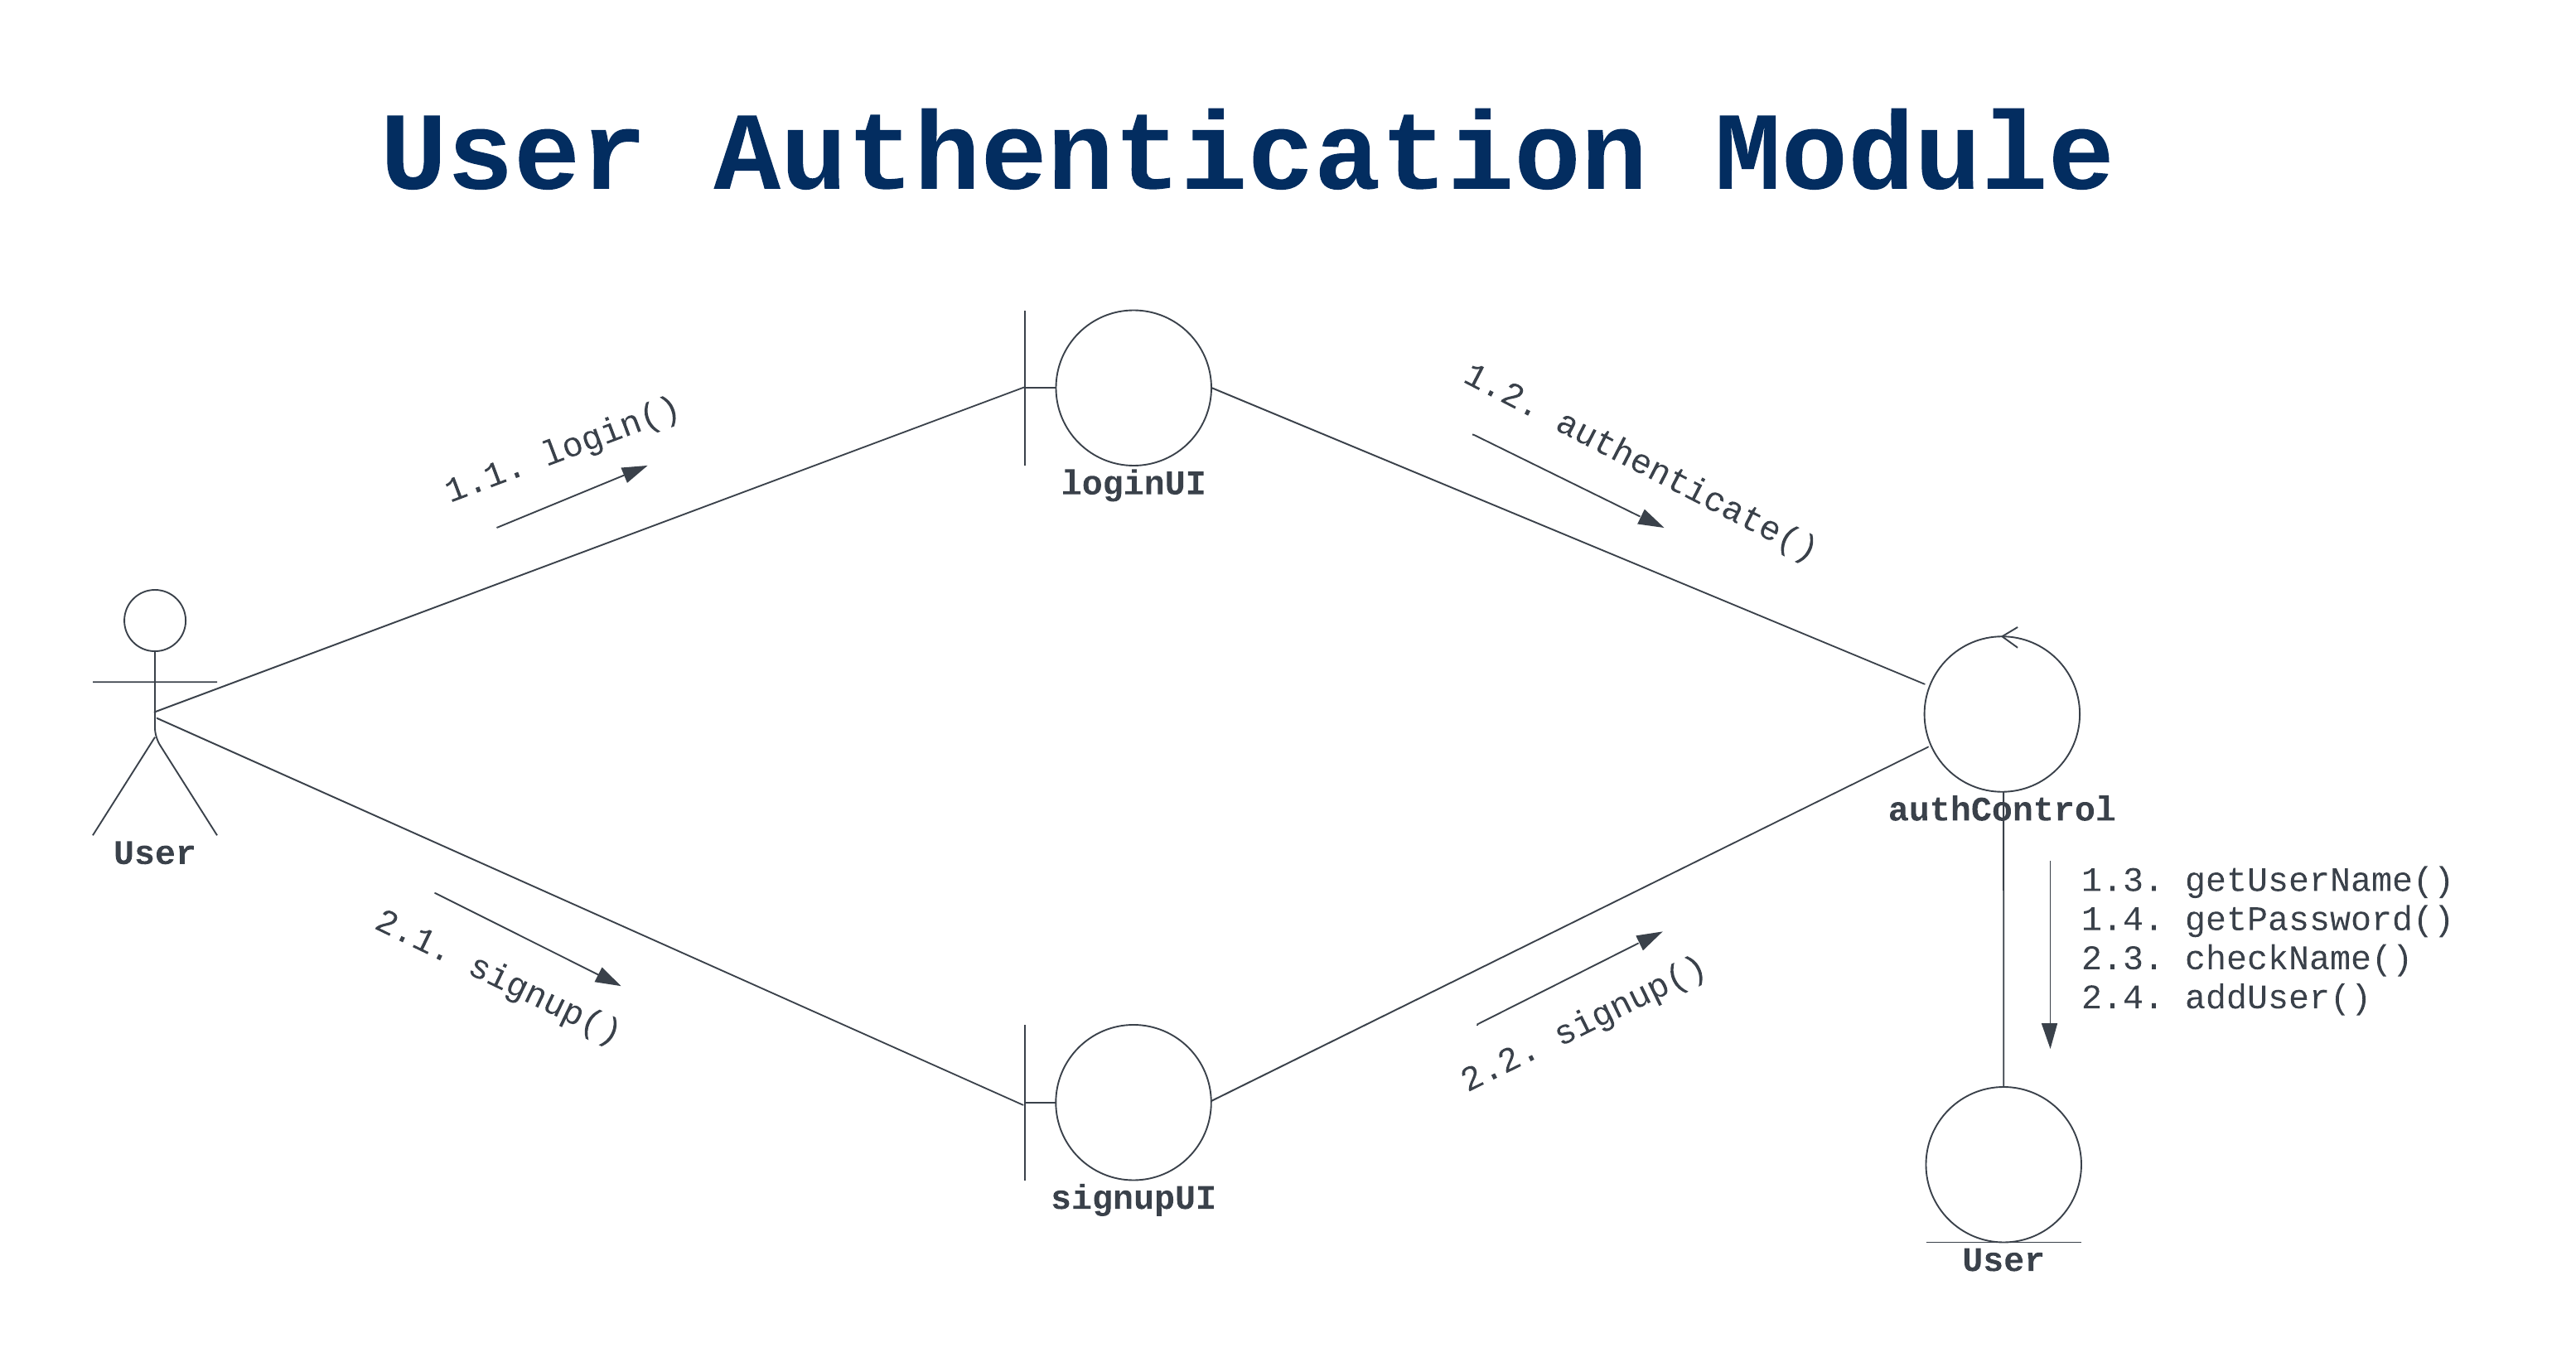
\includegraphics[width=0.95\textwidth]{Collaboration Diagram/Authentication.png}
        \label{fig:CollabAuth}
    \caption{Collaboration Diagram - User Authentication}
\end{figure}

\subsection{Profile Dashboard}
\begin{figure}[H]
    \centering
        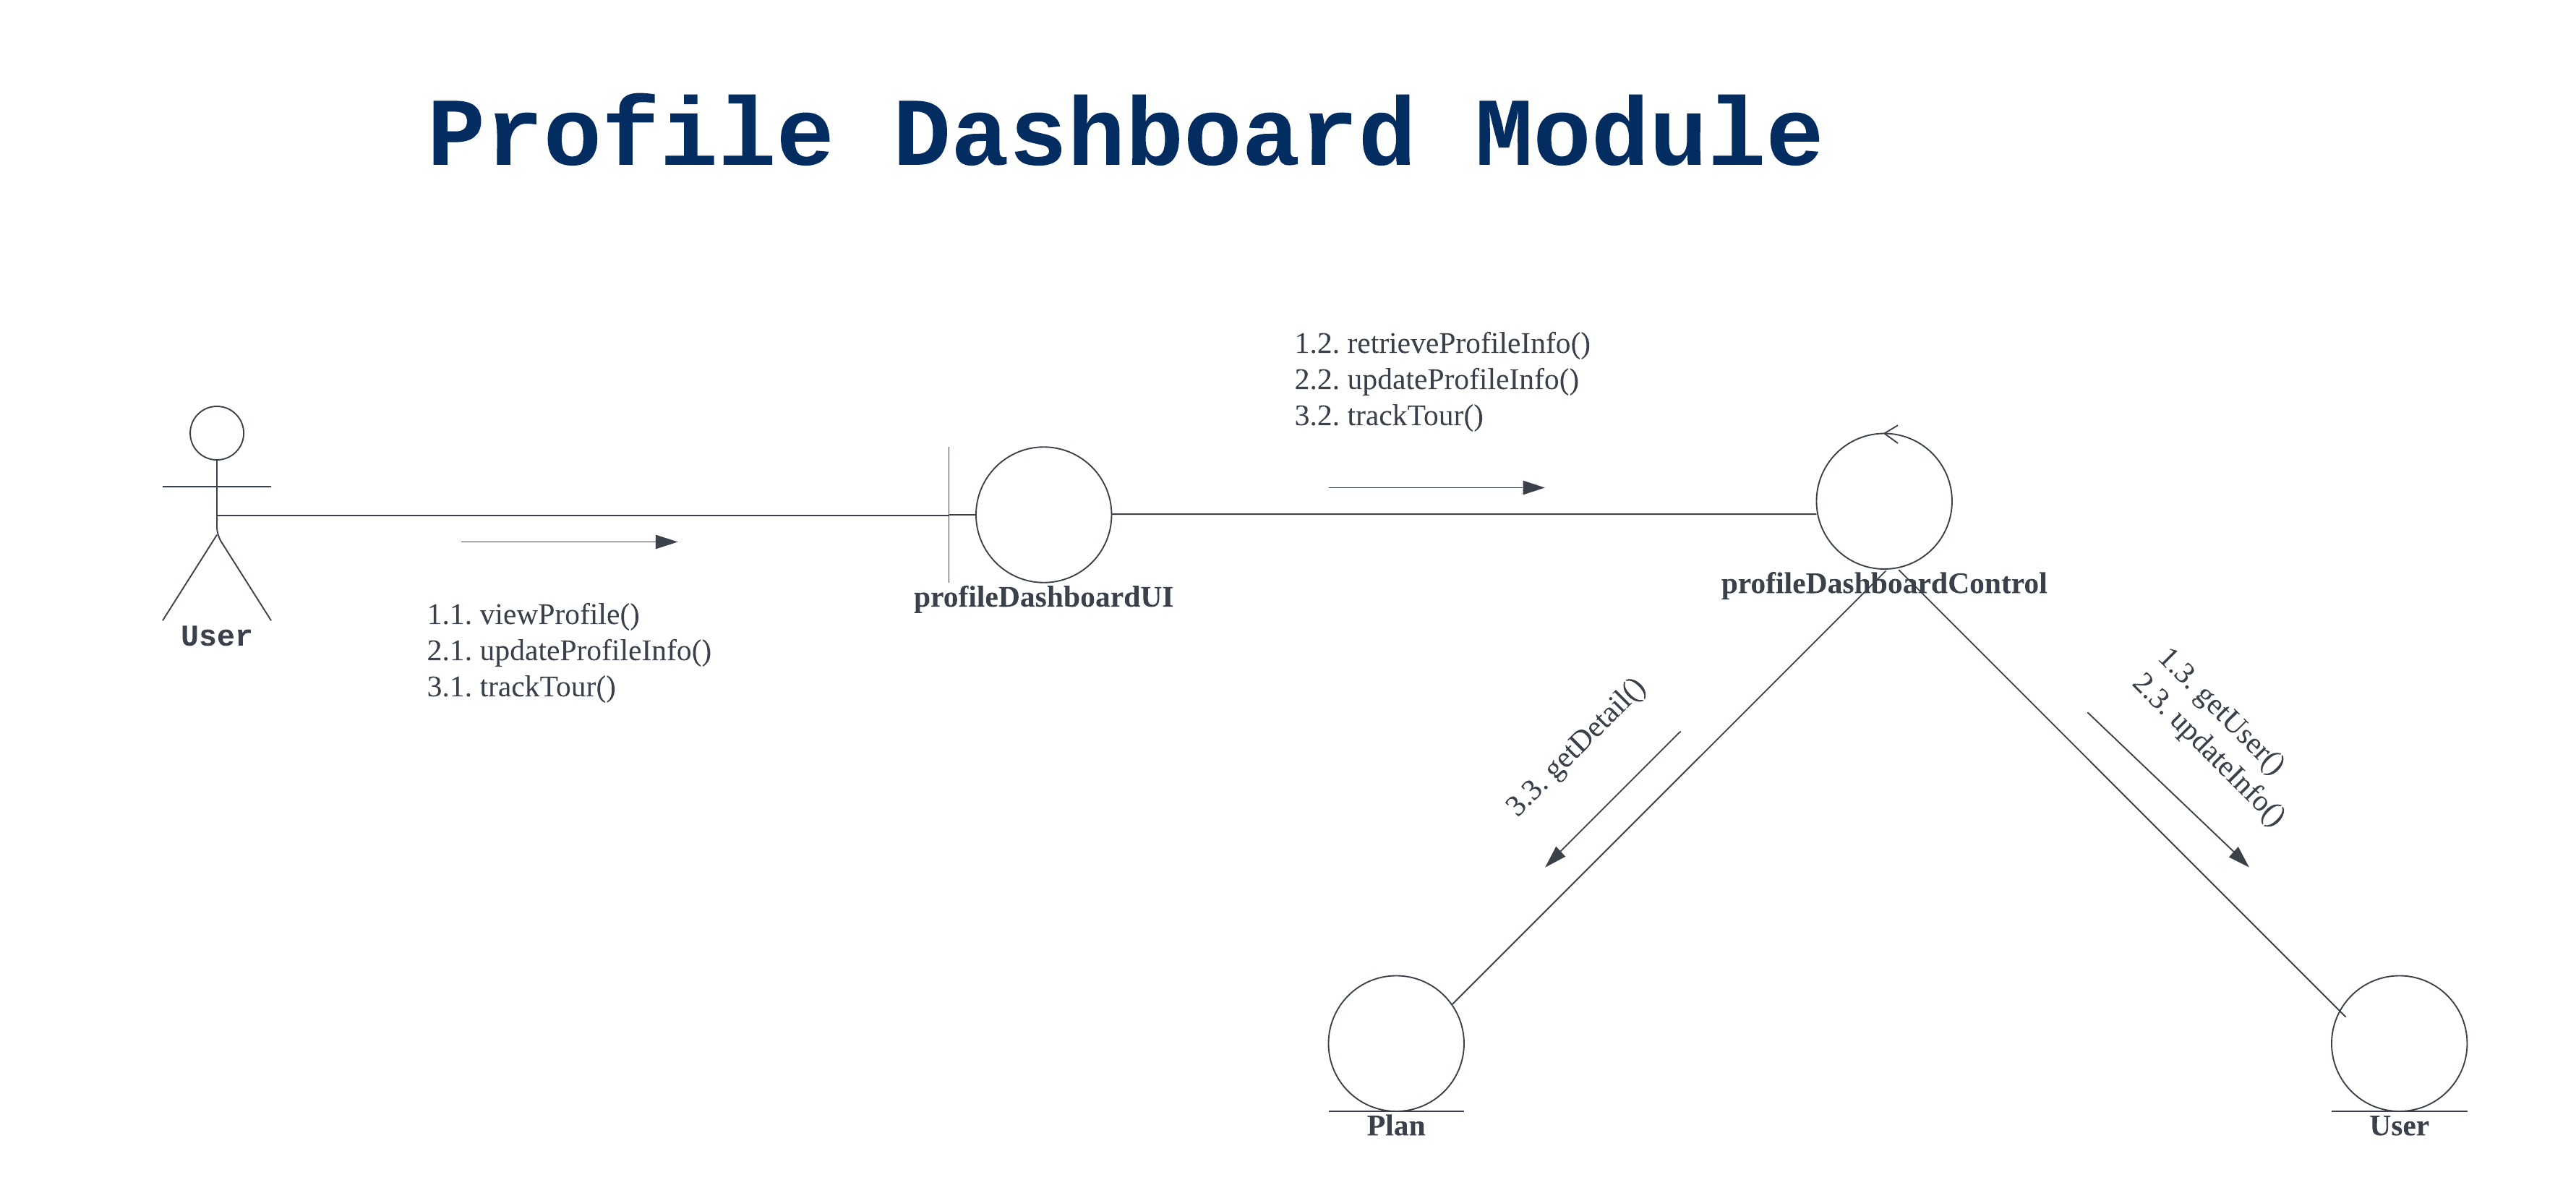
\includegraphics[width=0.95\textwidth]{Collaboration Diagram/Profile Dashboard.png}
        \label{fig:CollabDash}
    \caption{Collaboration Diagram - Profile Dashboard}
\end{figure}

\newpage
\subsection{Destinations}
\begin{figure}[H]
    \centering
        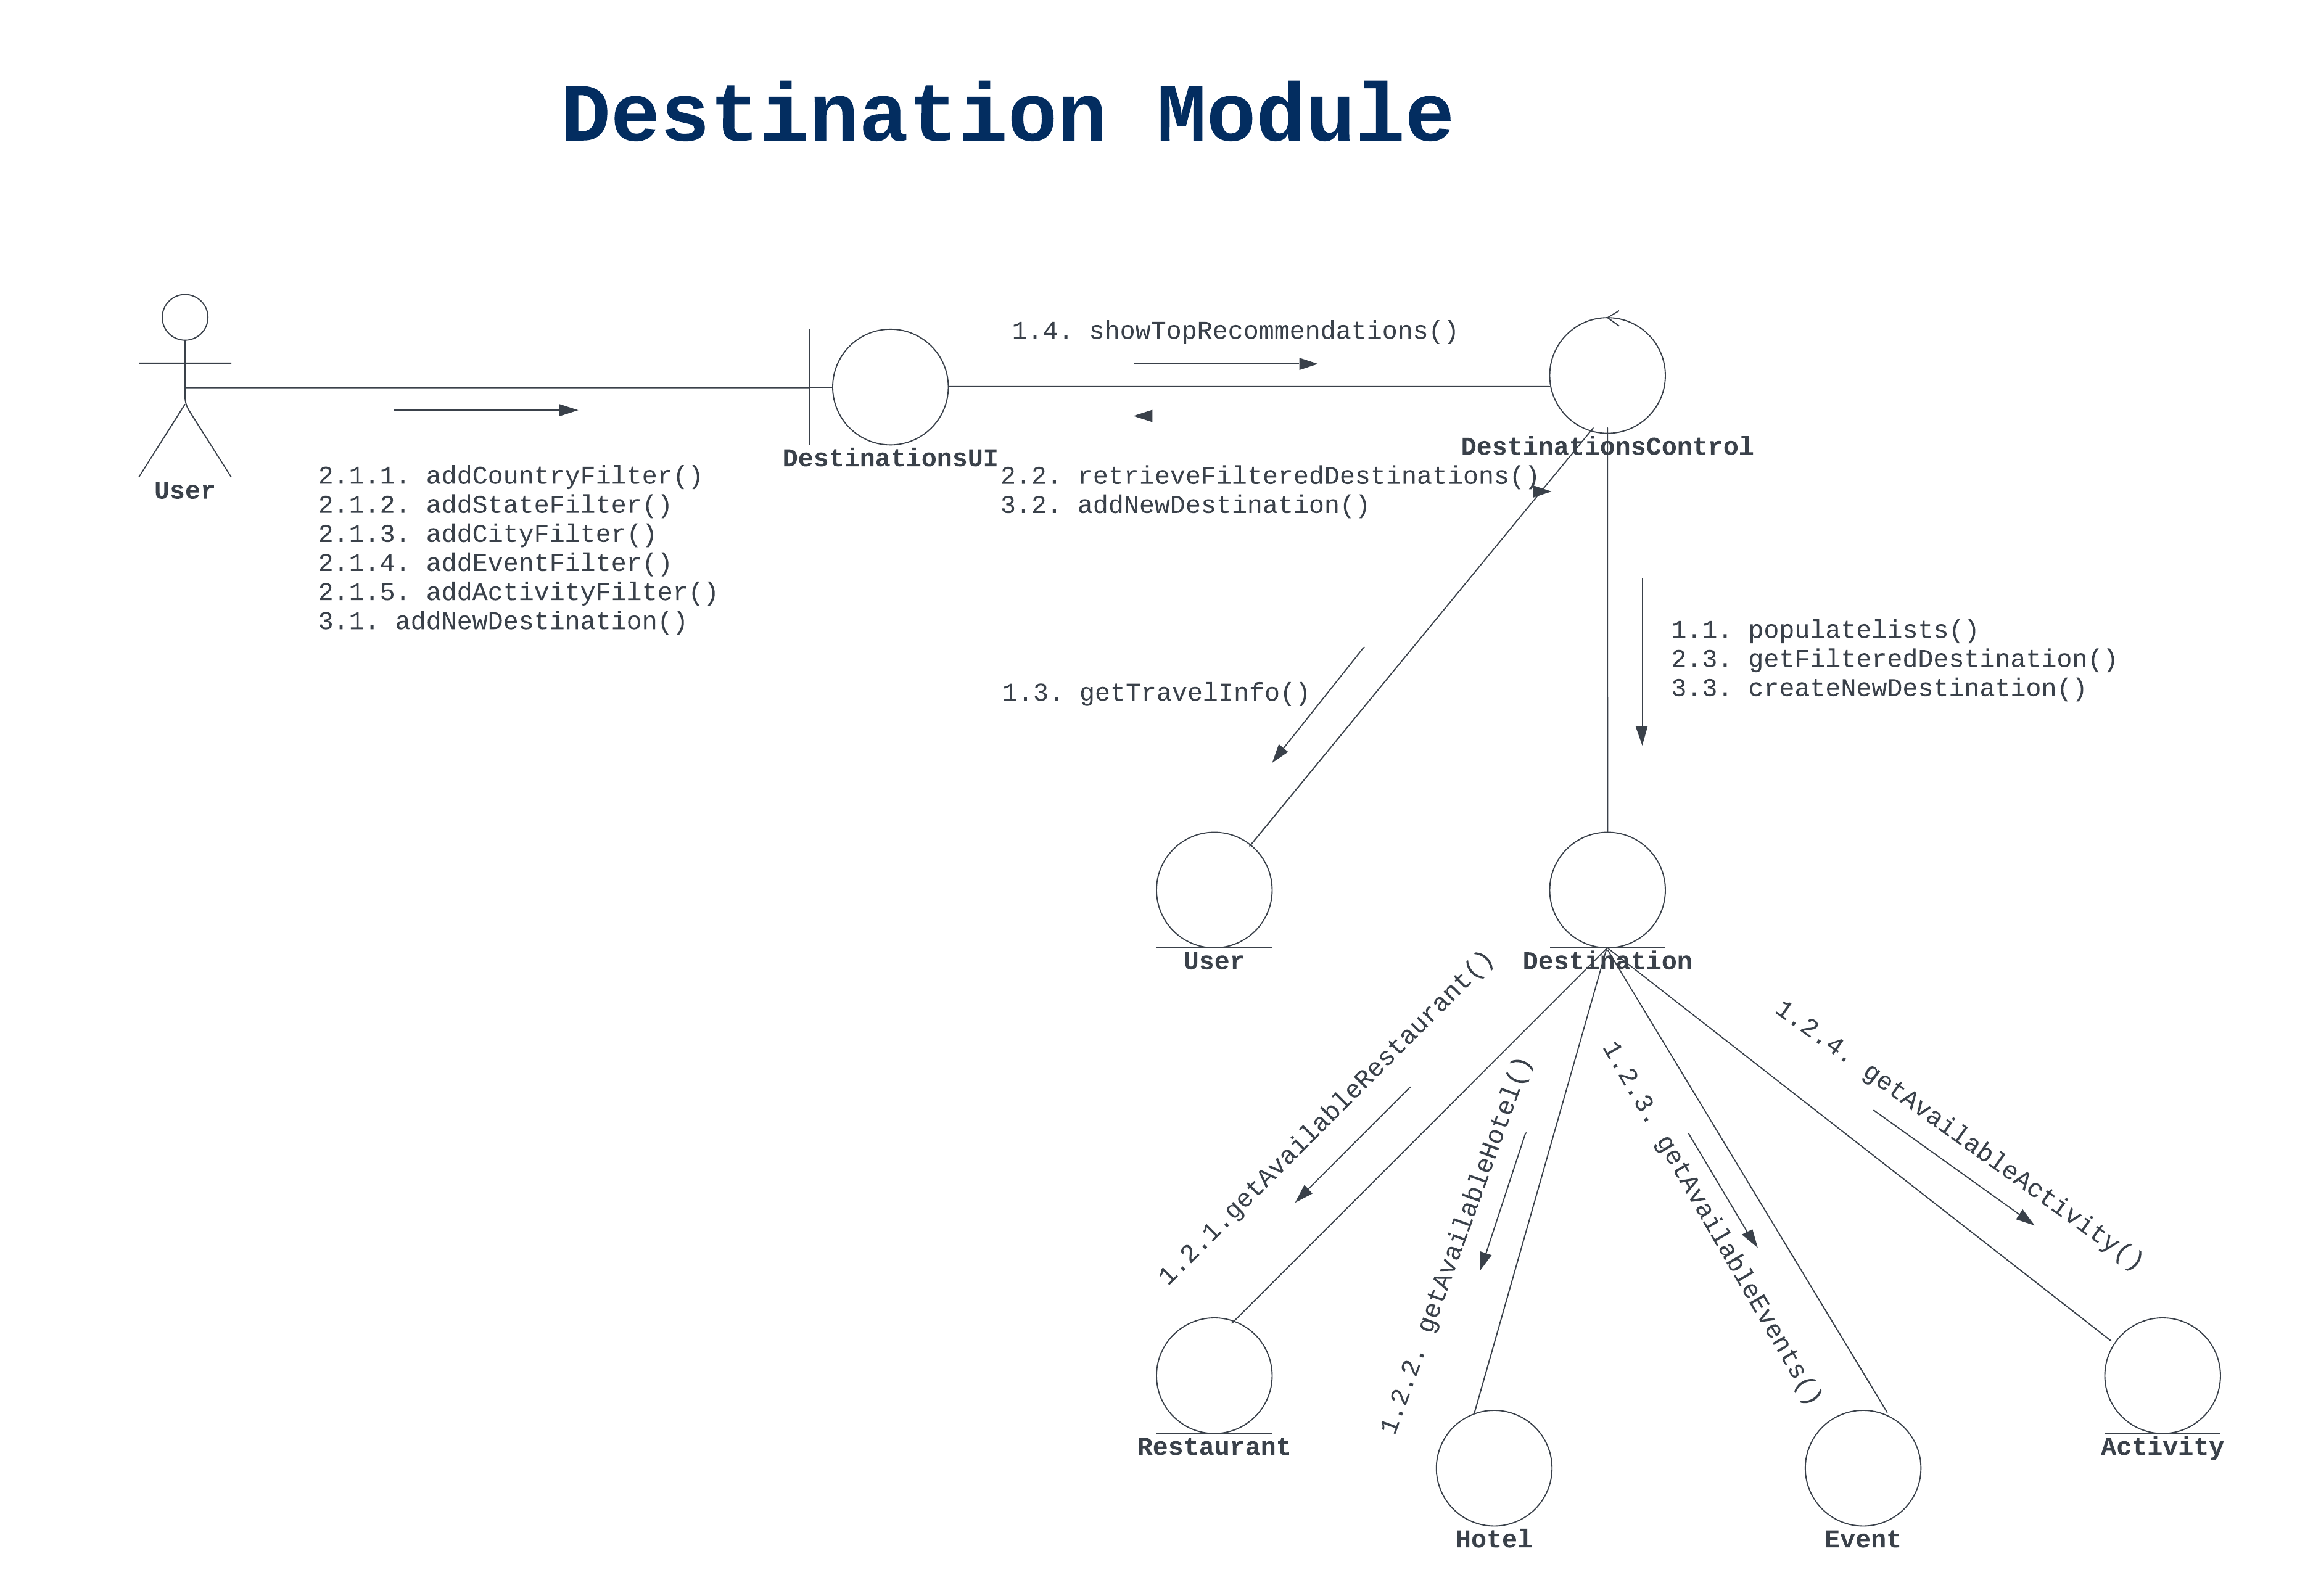
\includegraphics[width=0.95\textwidth]{Collaboration Diagram/Destinations.png}
        \label{fig:CollabDest}
    \caption{Collaboration Diagram - Destinations}
\end{figure}

\subsection{Destination Details}
\begin{figure}[H]
    \centering
        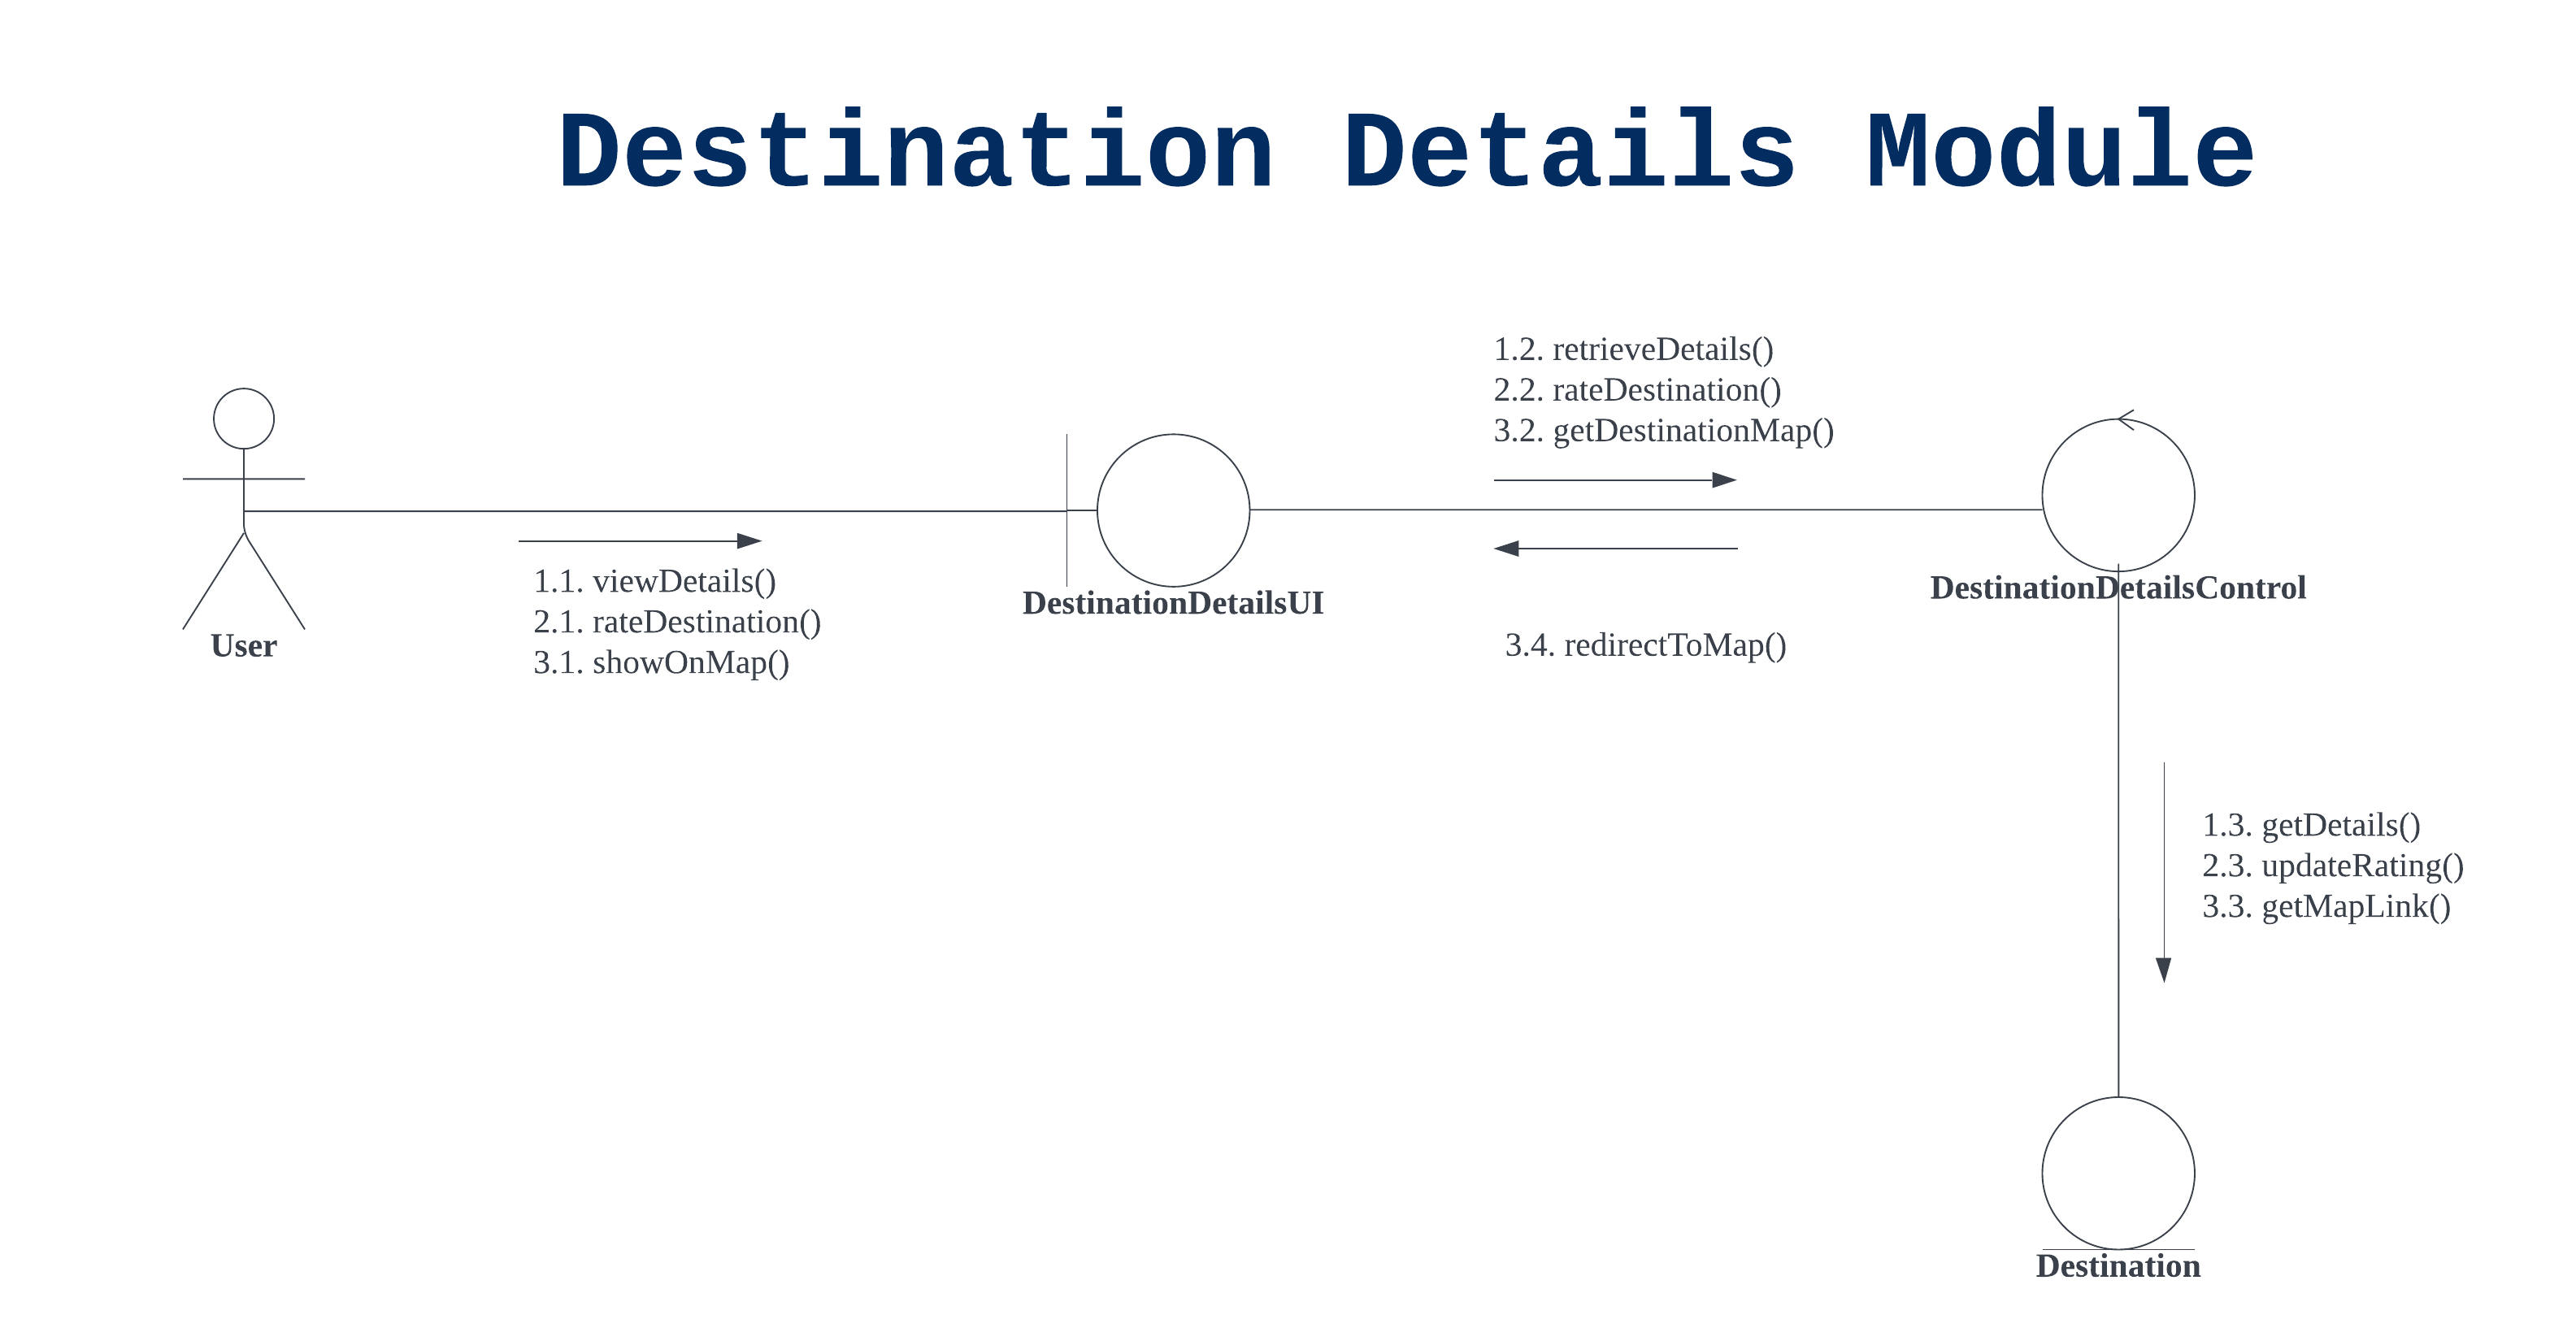
\includegraphics[width=0.95\textwidth]{Collaboration Diagram/Destination Details.png}
        \label{fig:CollabDestDetails}
    \caption{Collaboration Diagram - Destination Details}
\end{figure}

\newpage
\subsection{Plans}
\begin{figure}[H]
    \centering
        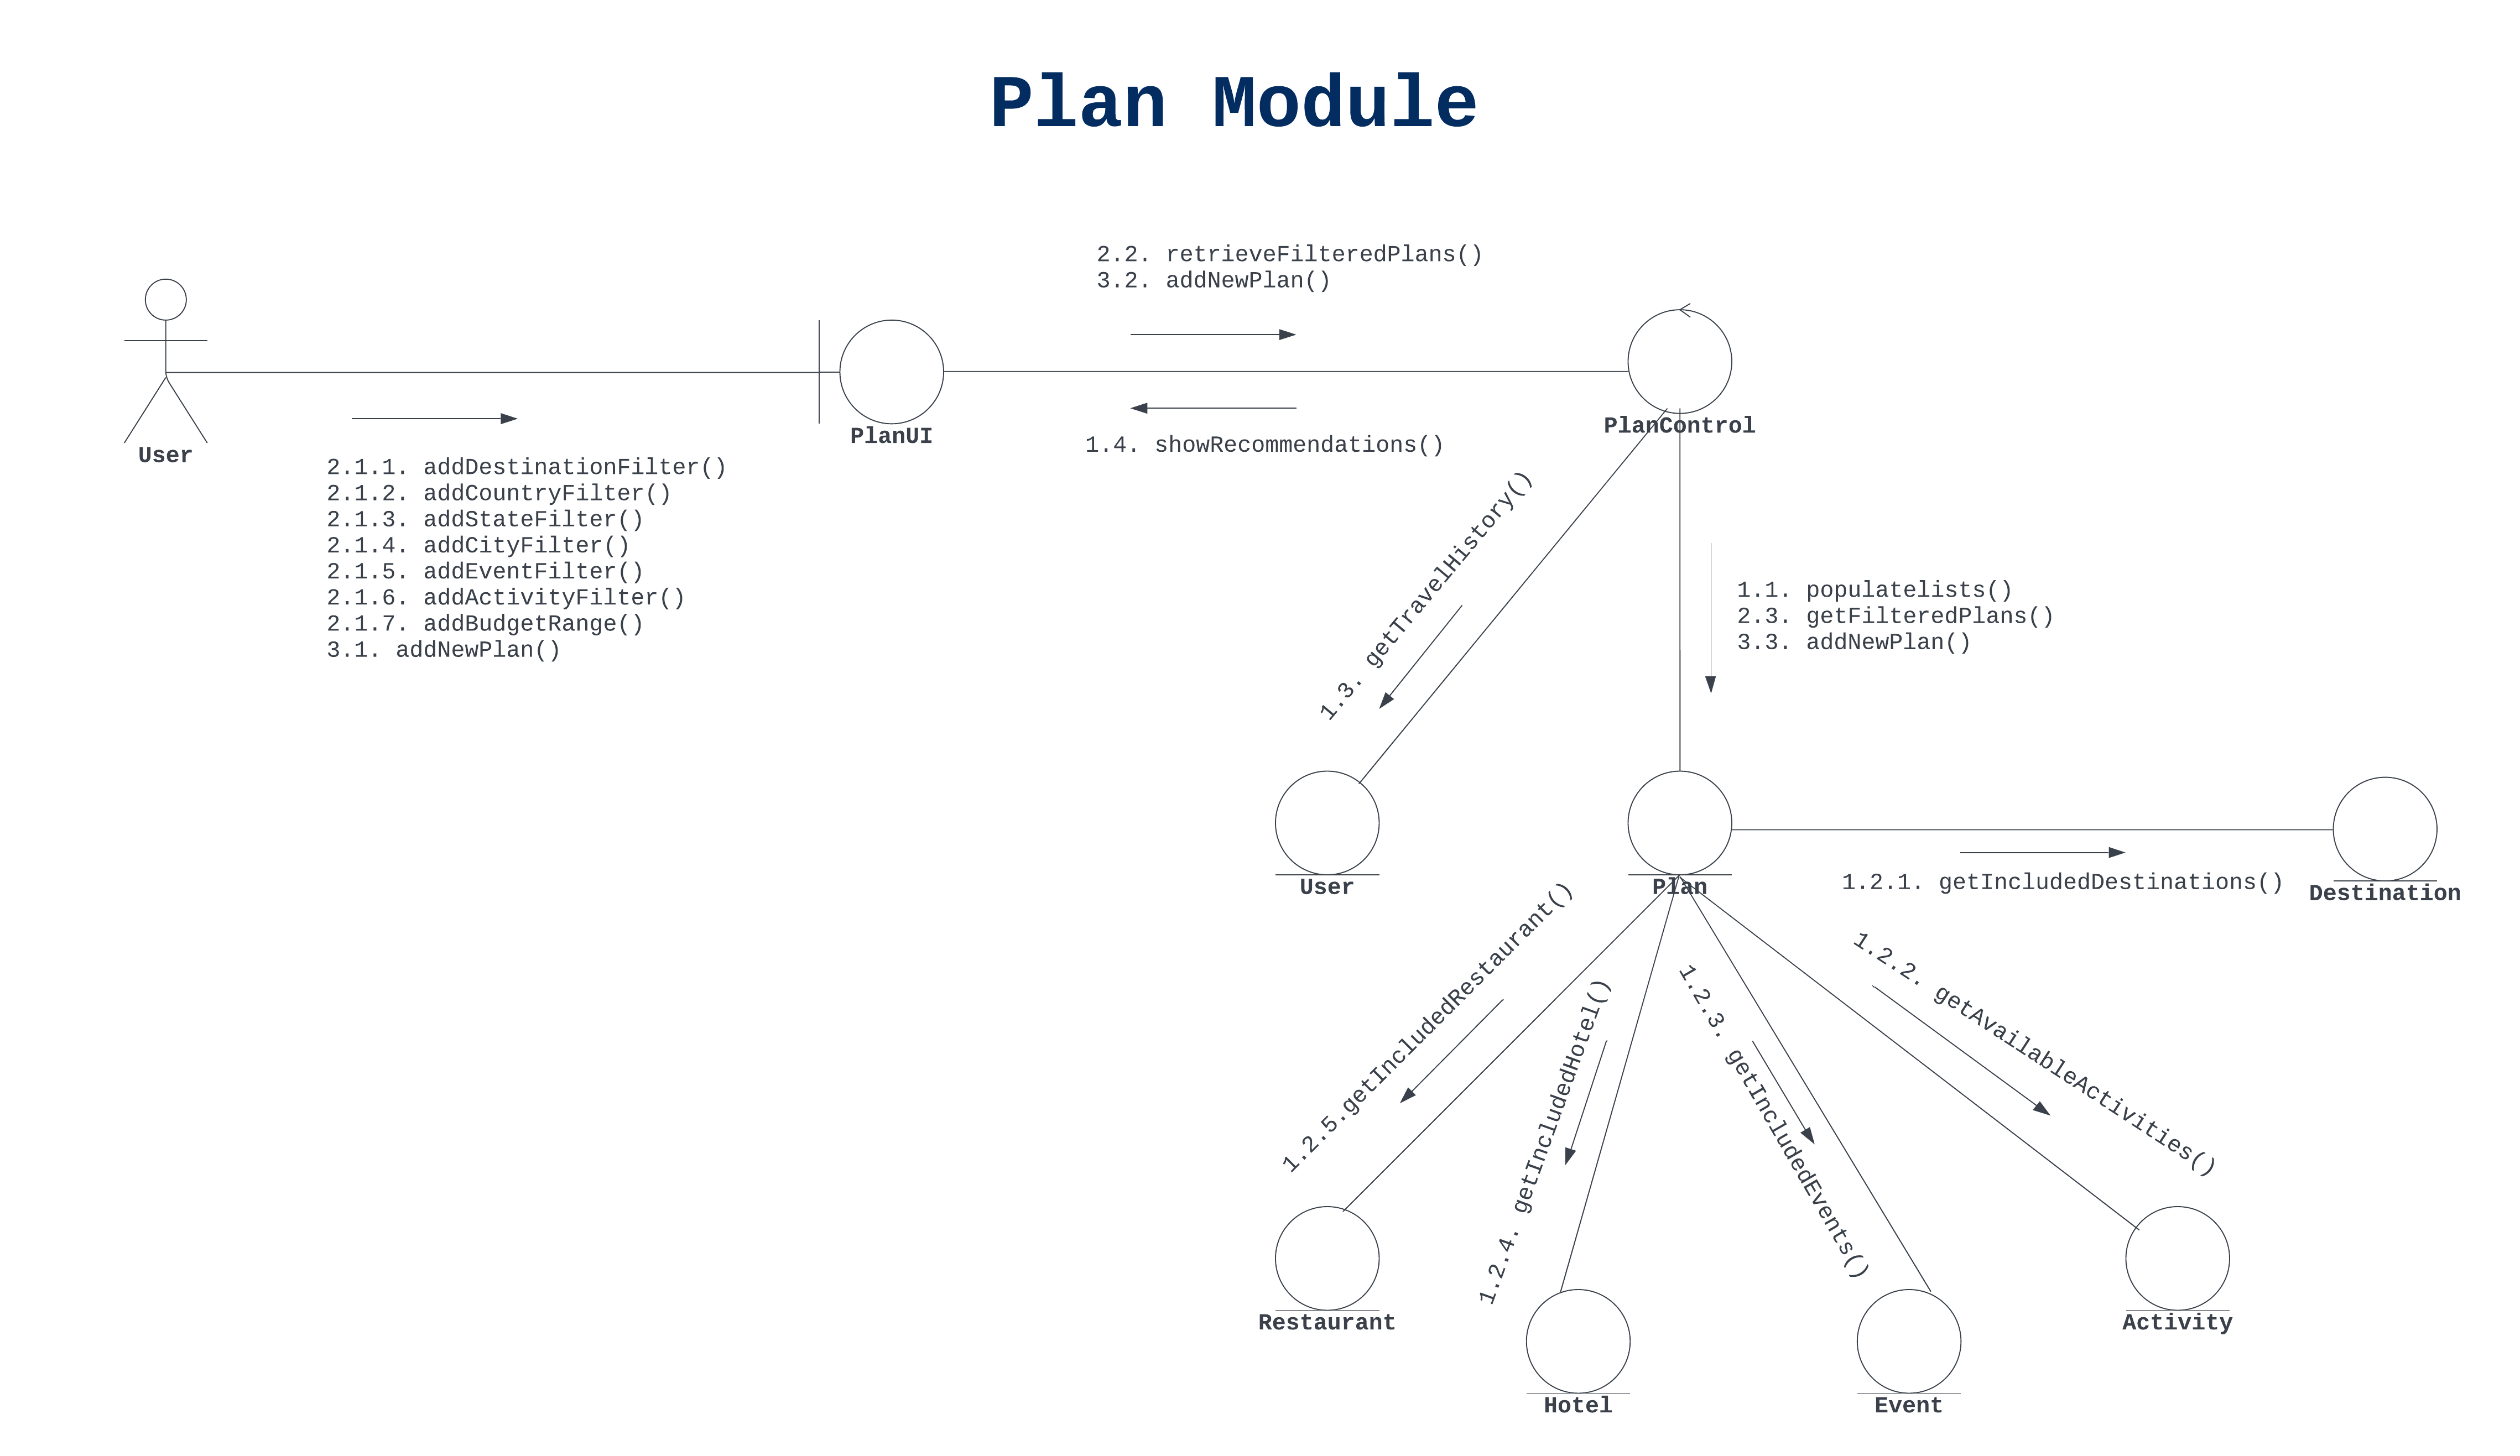
\includegraphics[width=0.95\textwidth]{Collaboration Diagram/Plans.png}
        \label{fig:CollabPlans}
    \caption{Collaboration Diagram - Plans}
\end{figure}

\subsection{Plan Details}
\begin{figure}[H]
    \centering
        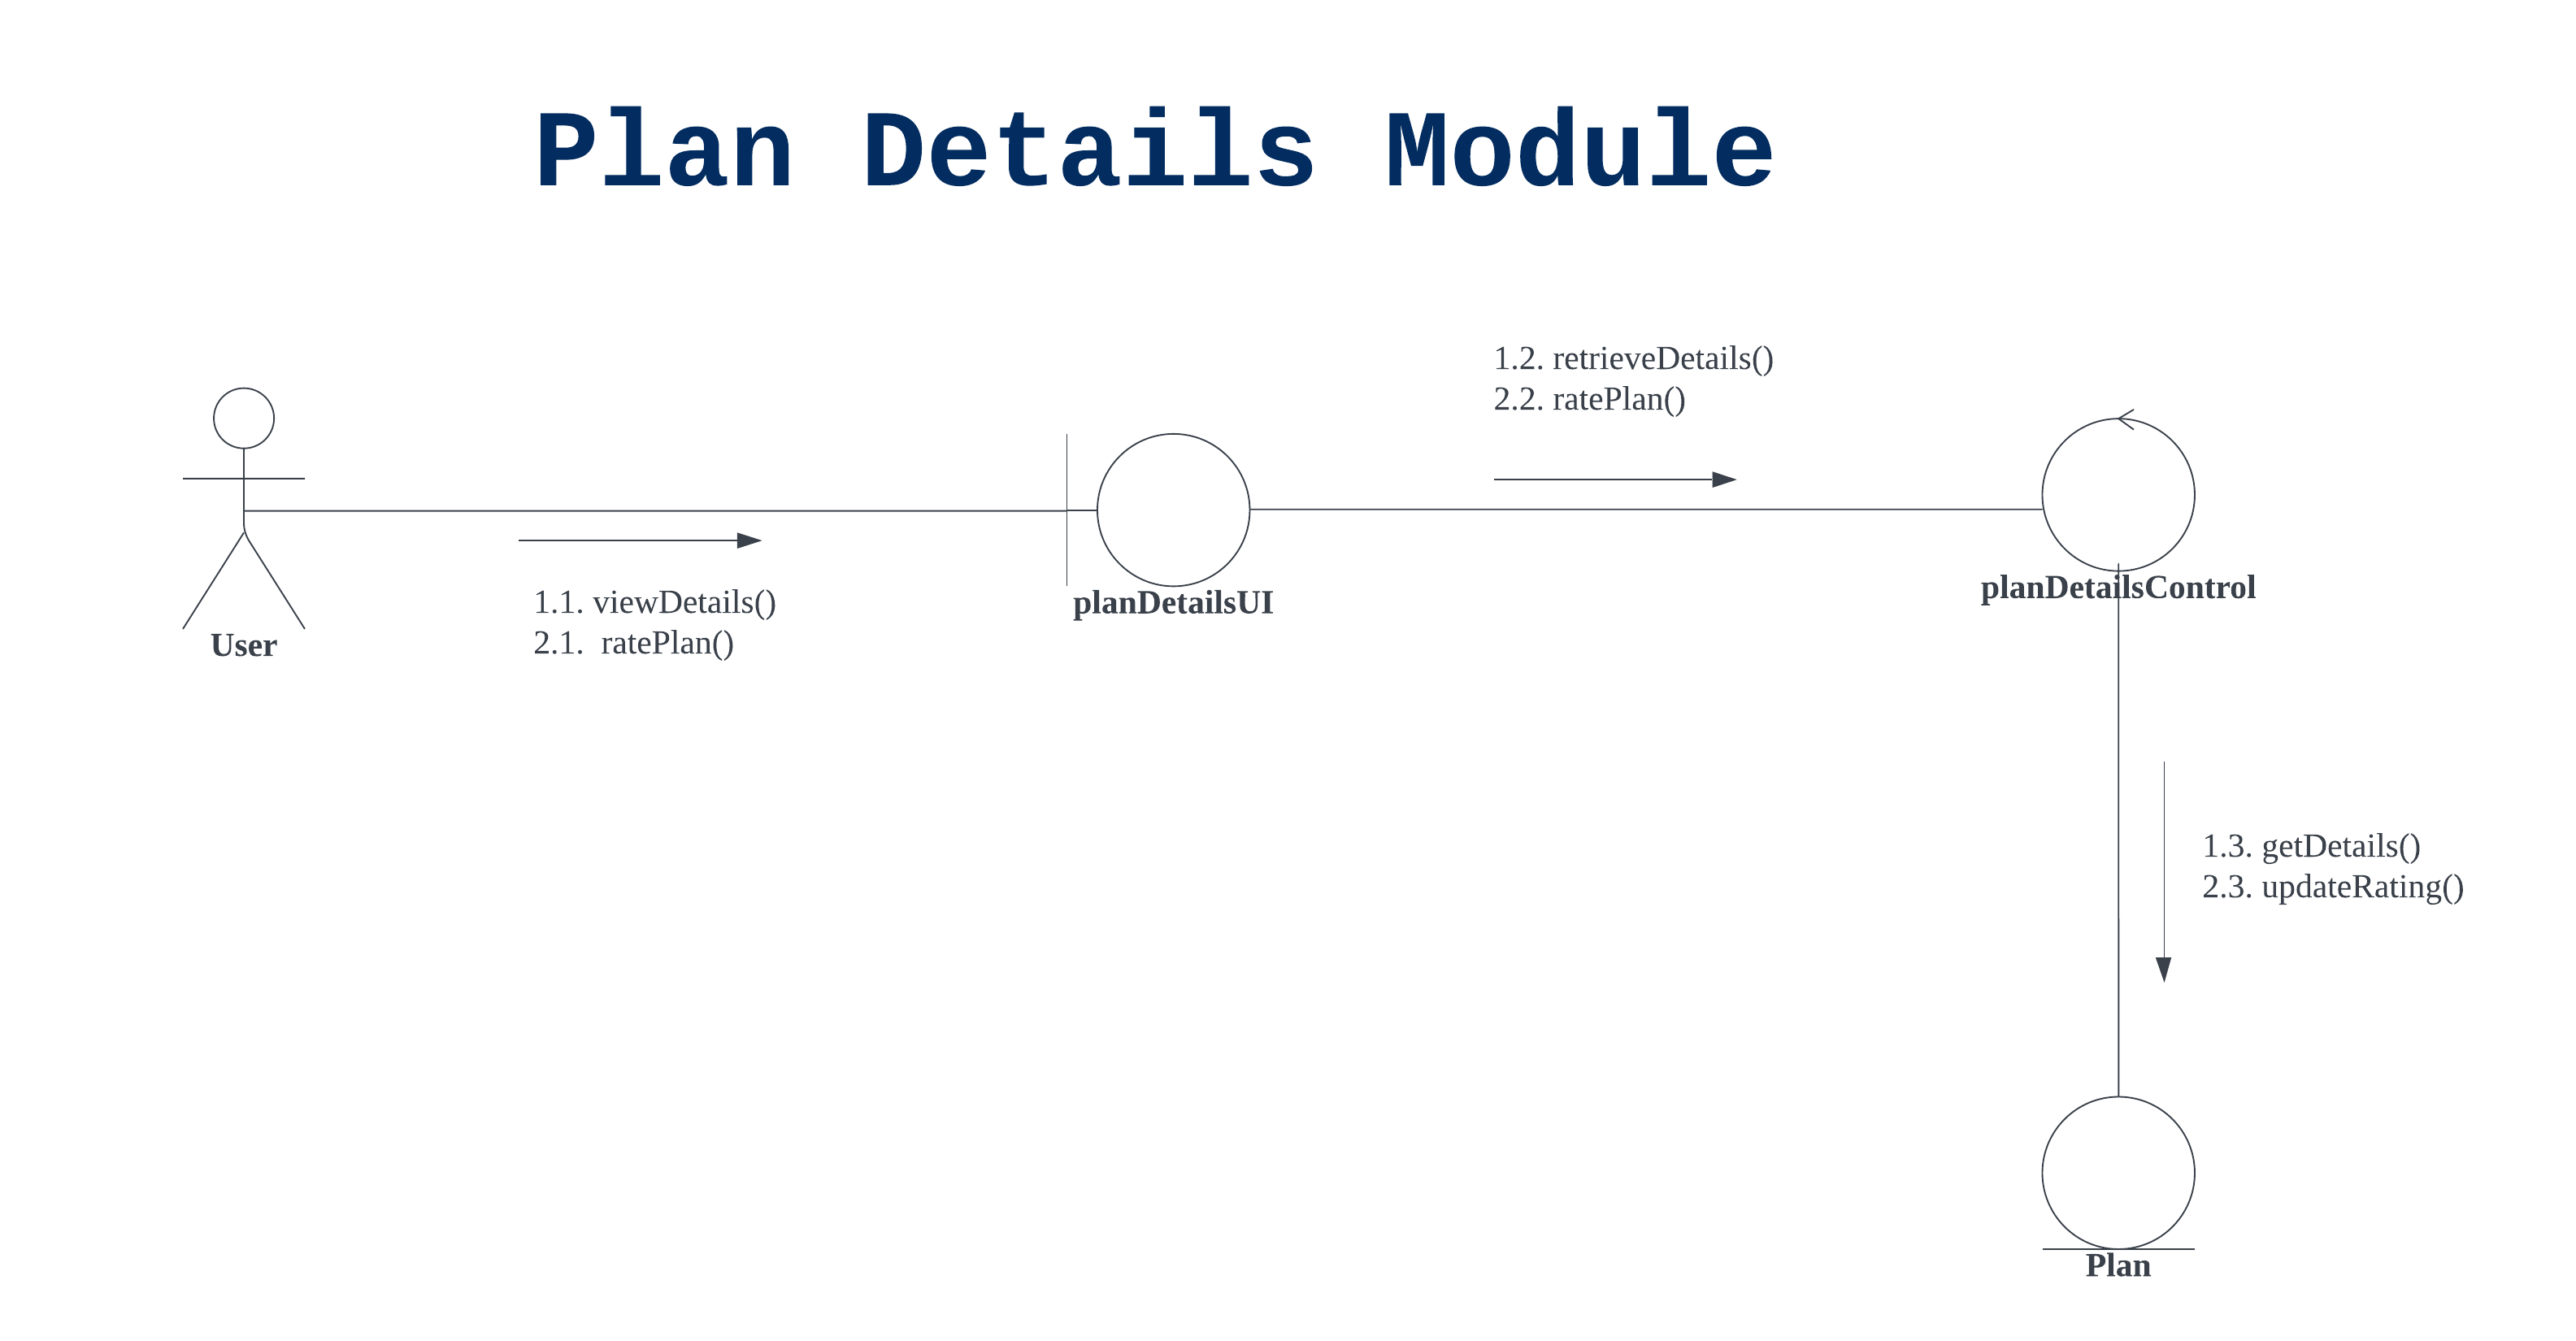
\includegraphics[width=0.95\textwidth]{Collaboration Diagram/Plan Details.png}
        \label{fig:CollabPlanDetails}
    \caption{Collaboration Diagram - Plan Details}
\end{figure}

\newpage
\subsection{Customize Plan}
\begin{figure}[H]
    \centering
        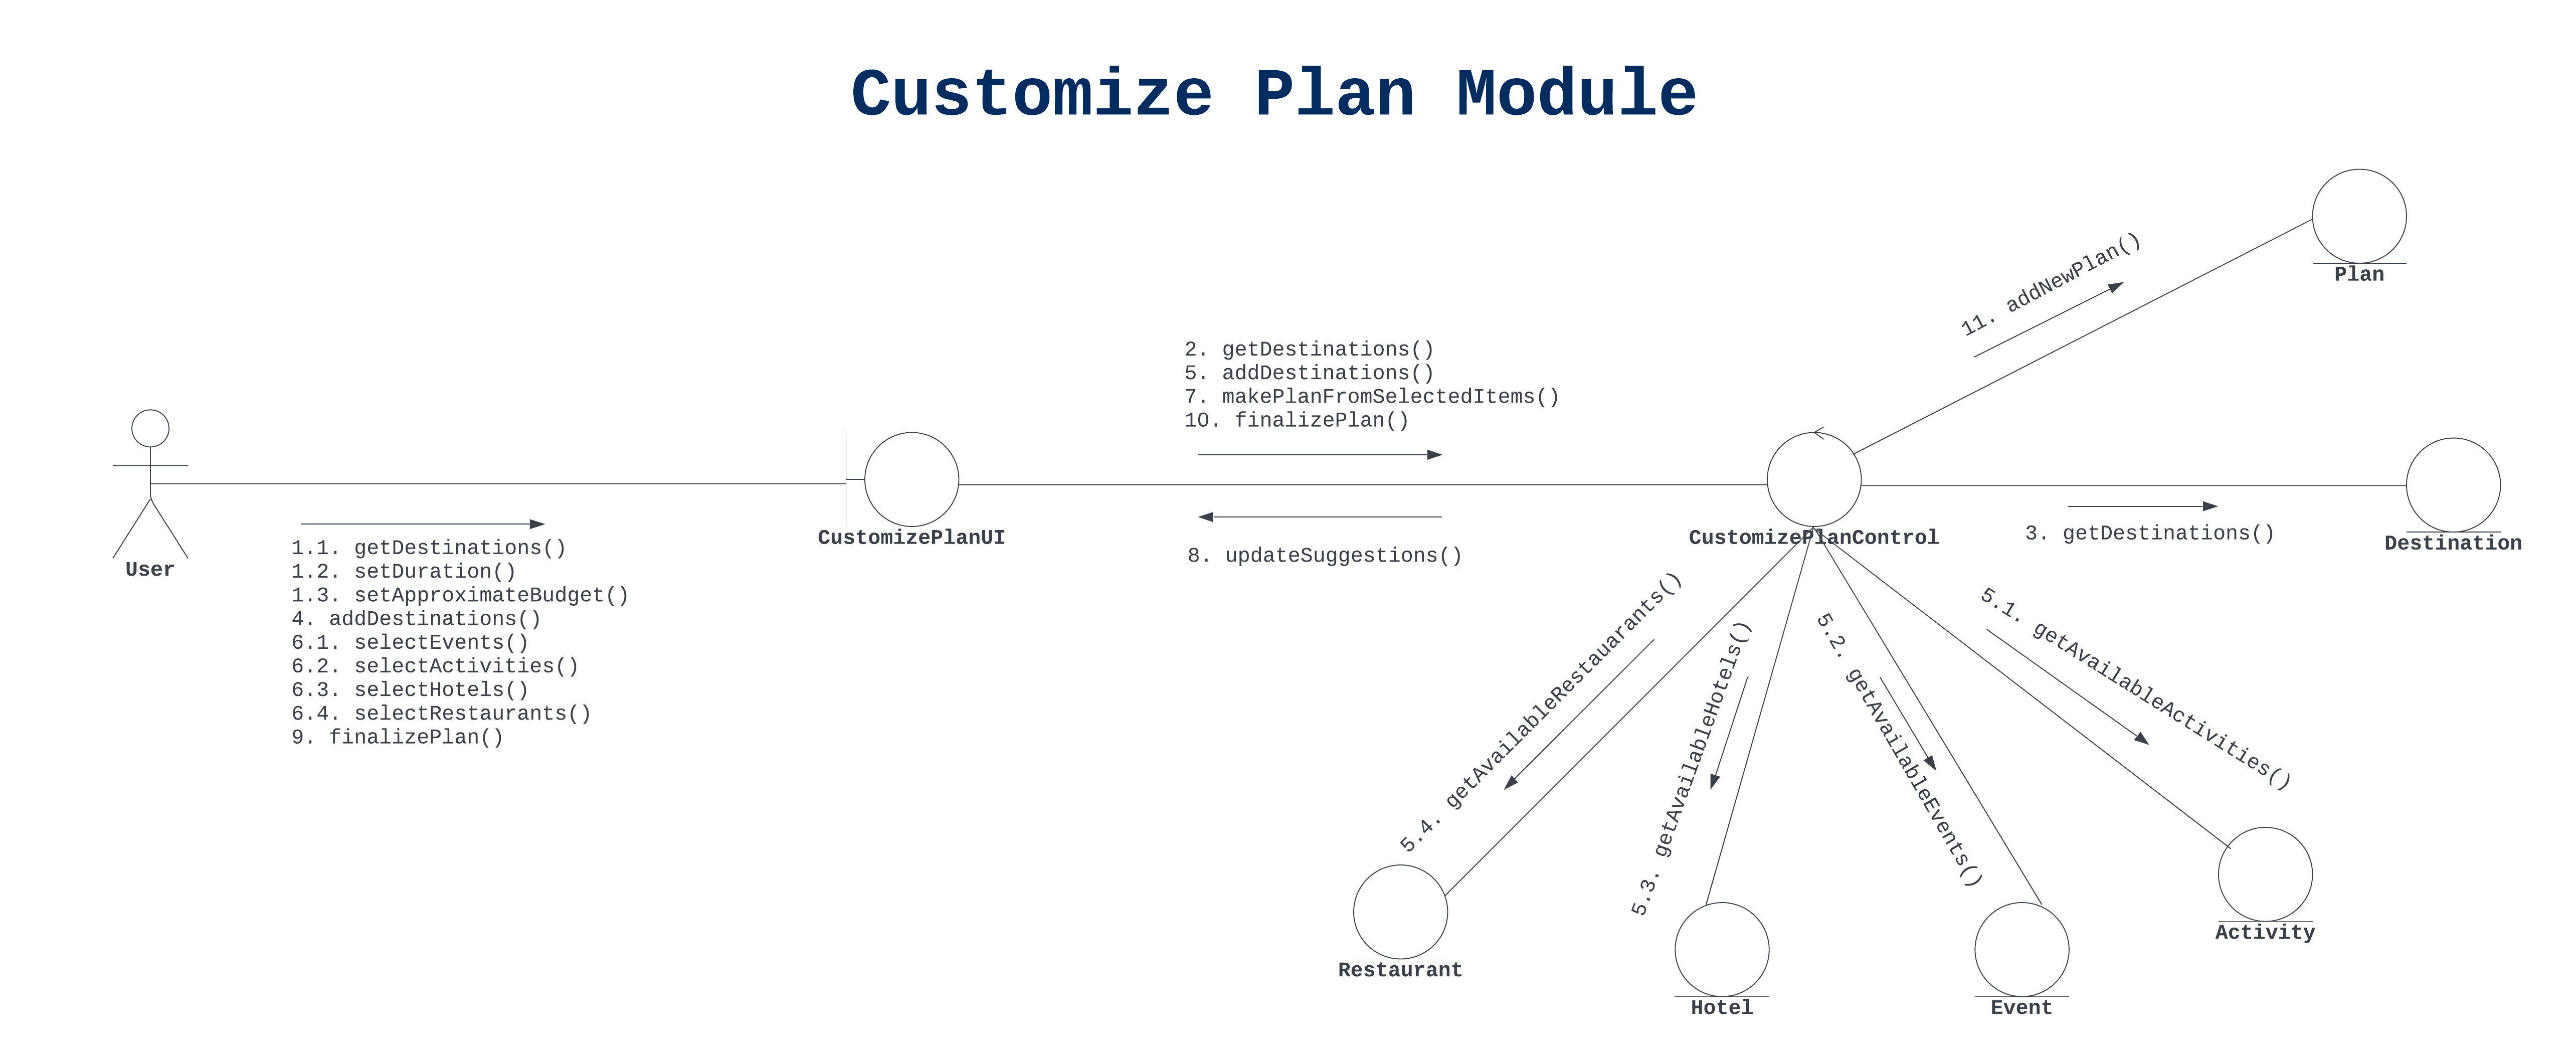
\includegraphics[width=0.95\textwidth]{Collaboration Diagram/Customize Plan.png}
        \label{fig:CollabCustomize}
    \caption{Collaboration Diagram - Customize Plan}
\end{figure}

\subsection{Tours}
\begin{figure}[H]
    \centering
        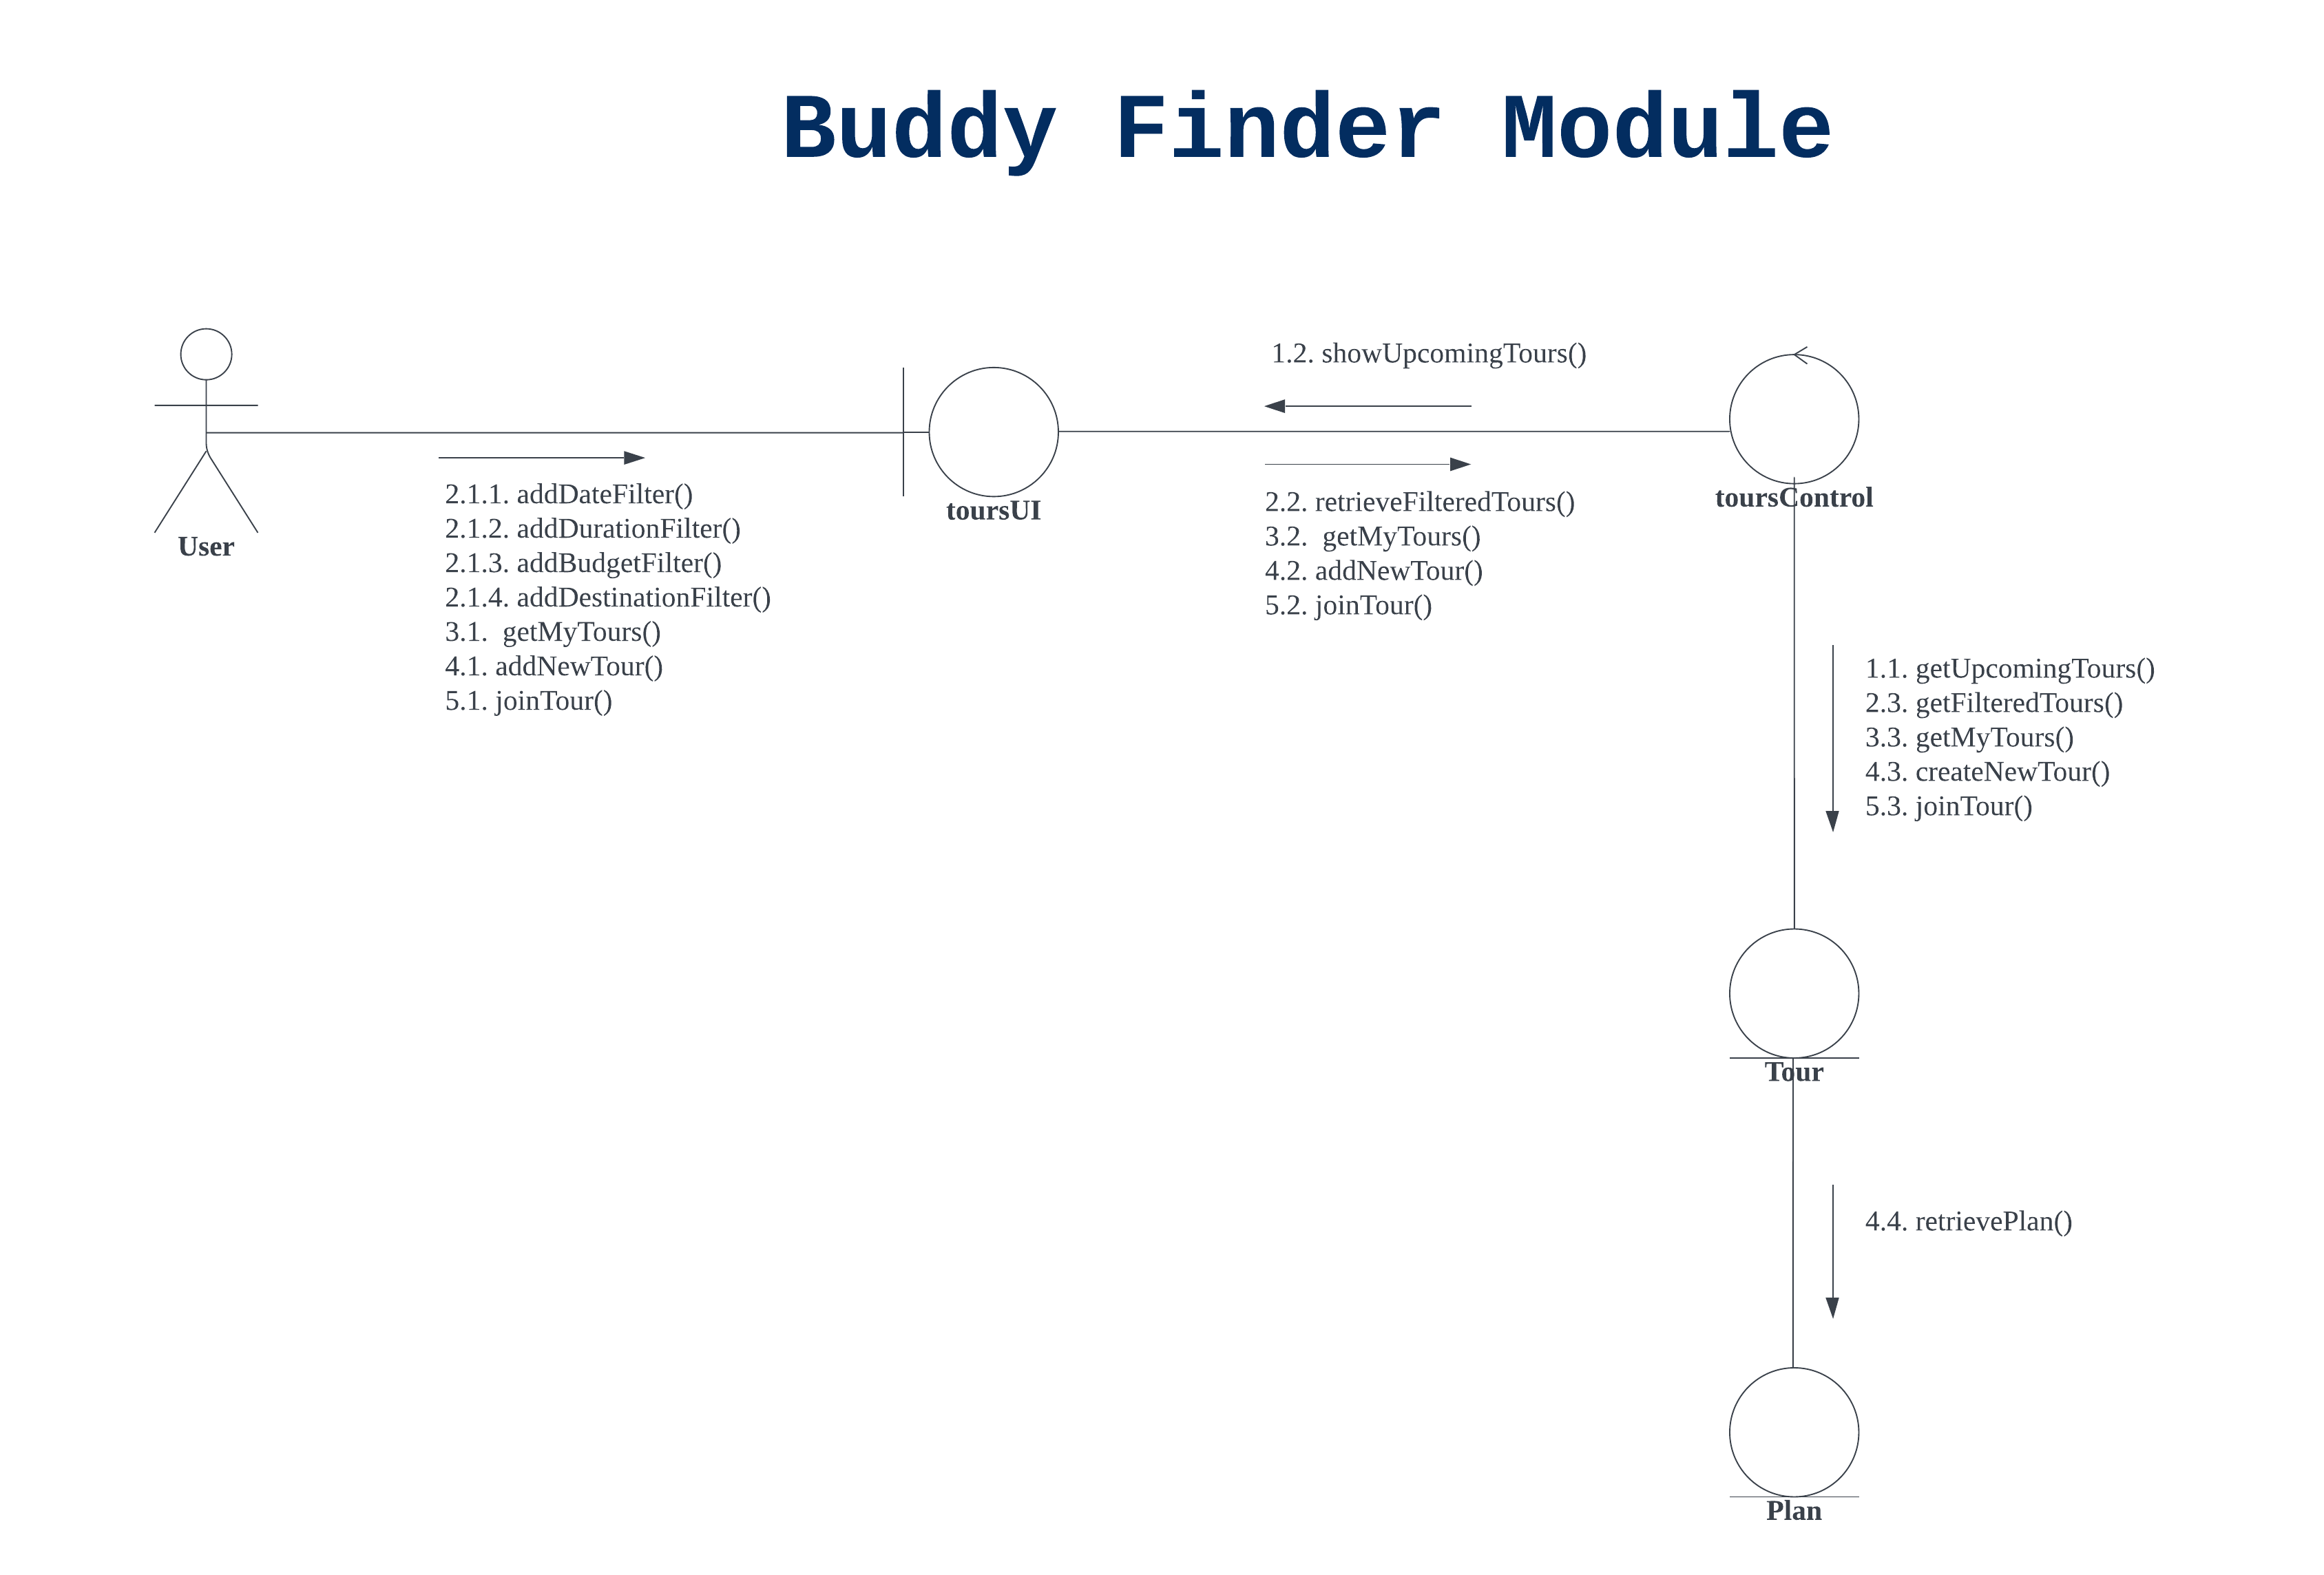
\includegraphics[width=0.95\textwidth]{Collaboration Diagram/Tours.png}
        \label{fig:CollabTour}
    \caption{Collaboration Diagram - Tours}
\end{figure}

\newpage

\section{State Diagrams}
\subsection{Feedbacks Acknowledged}

\begin{itemize}
    \item Tour cancellation is shown
\end{itemize}

\subsection{State Diagram for \emph{Plan} Class}
\begin{figure}[H]
    \centering
        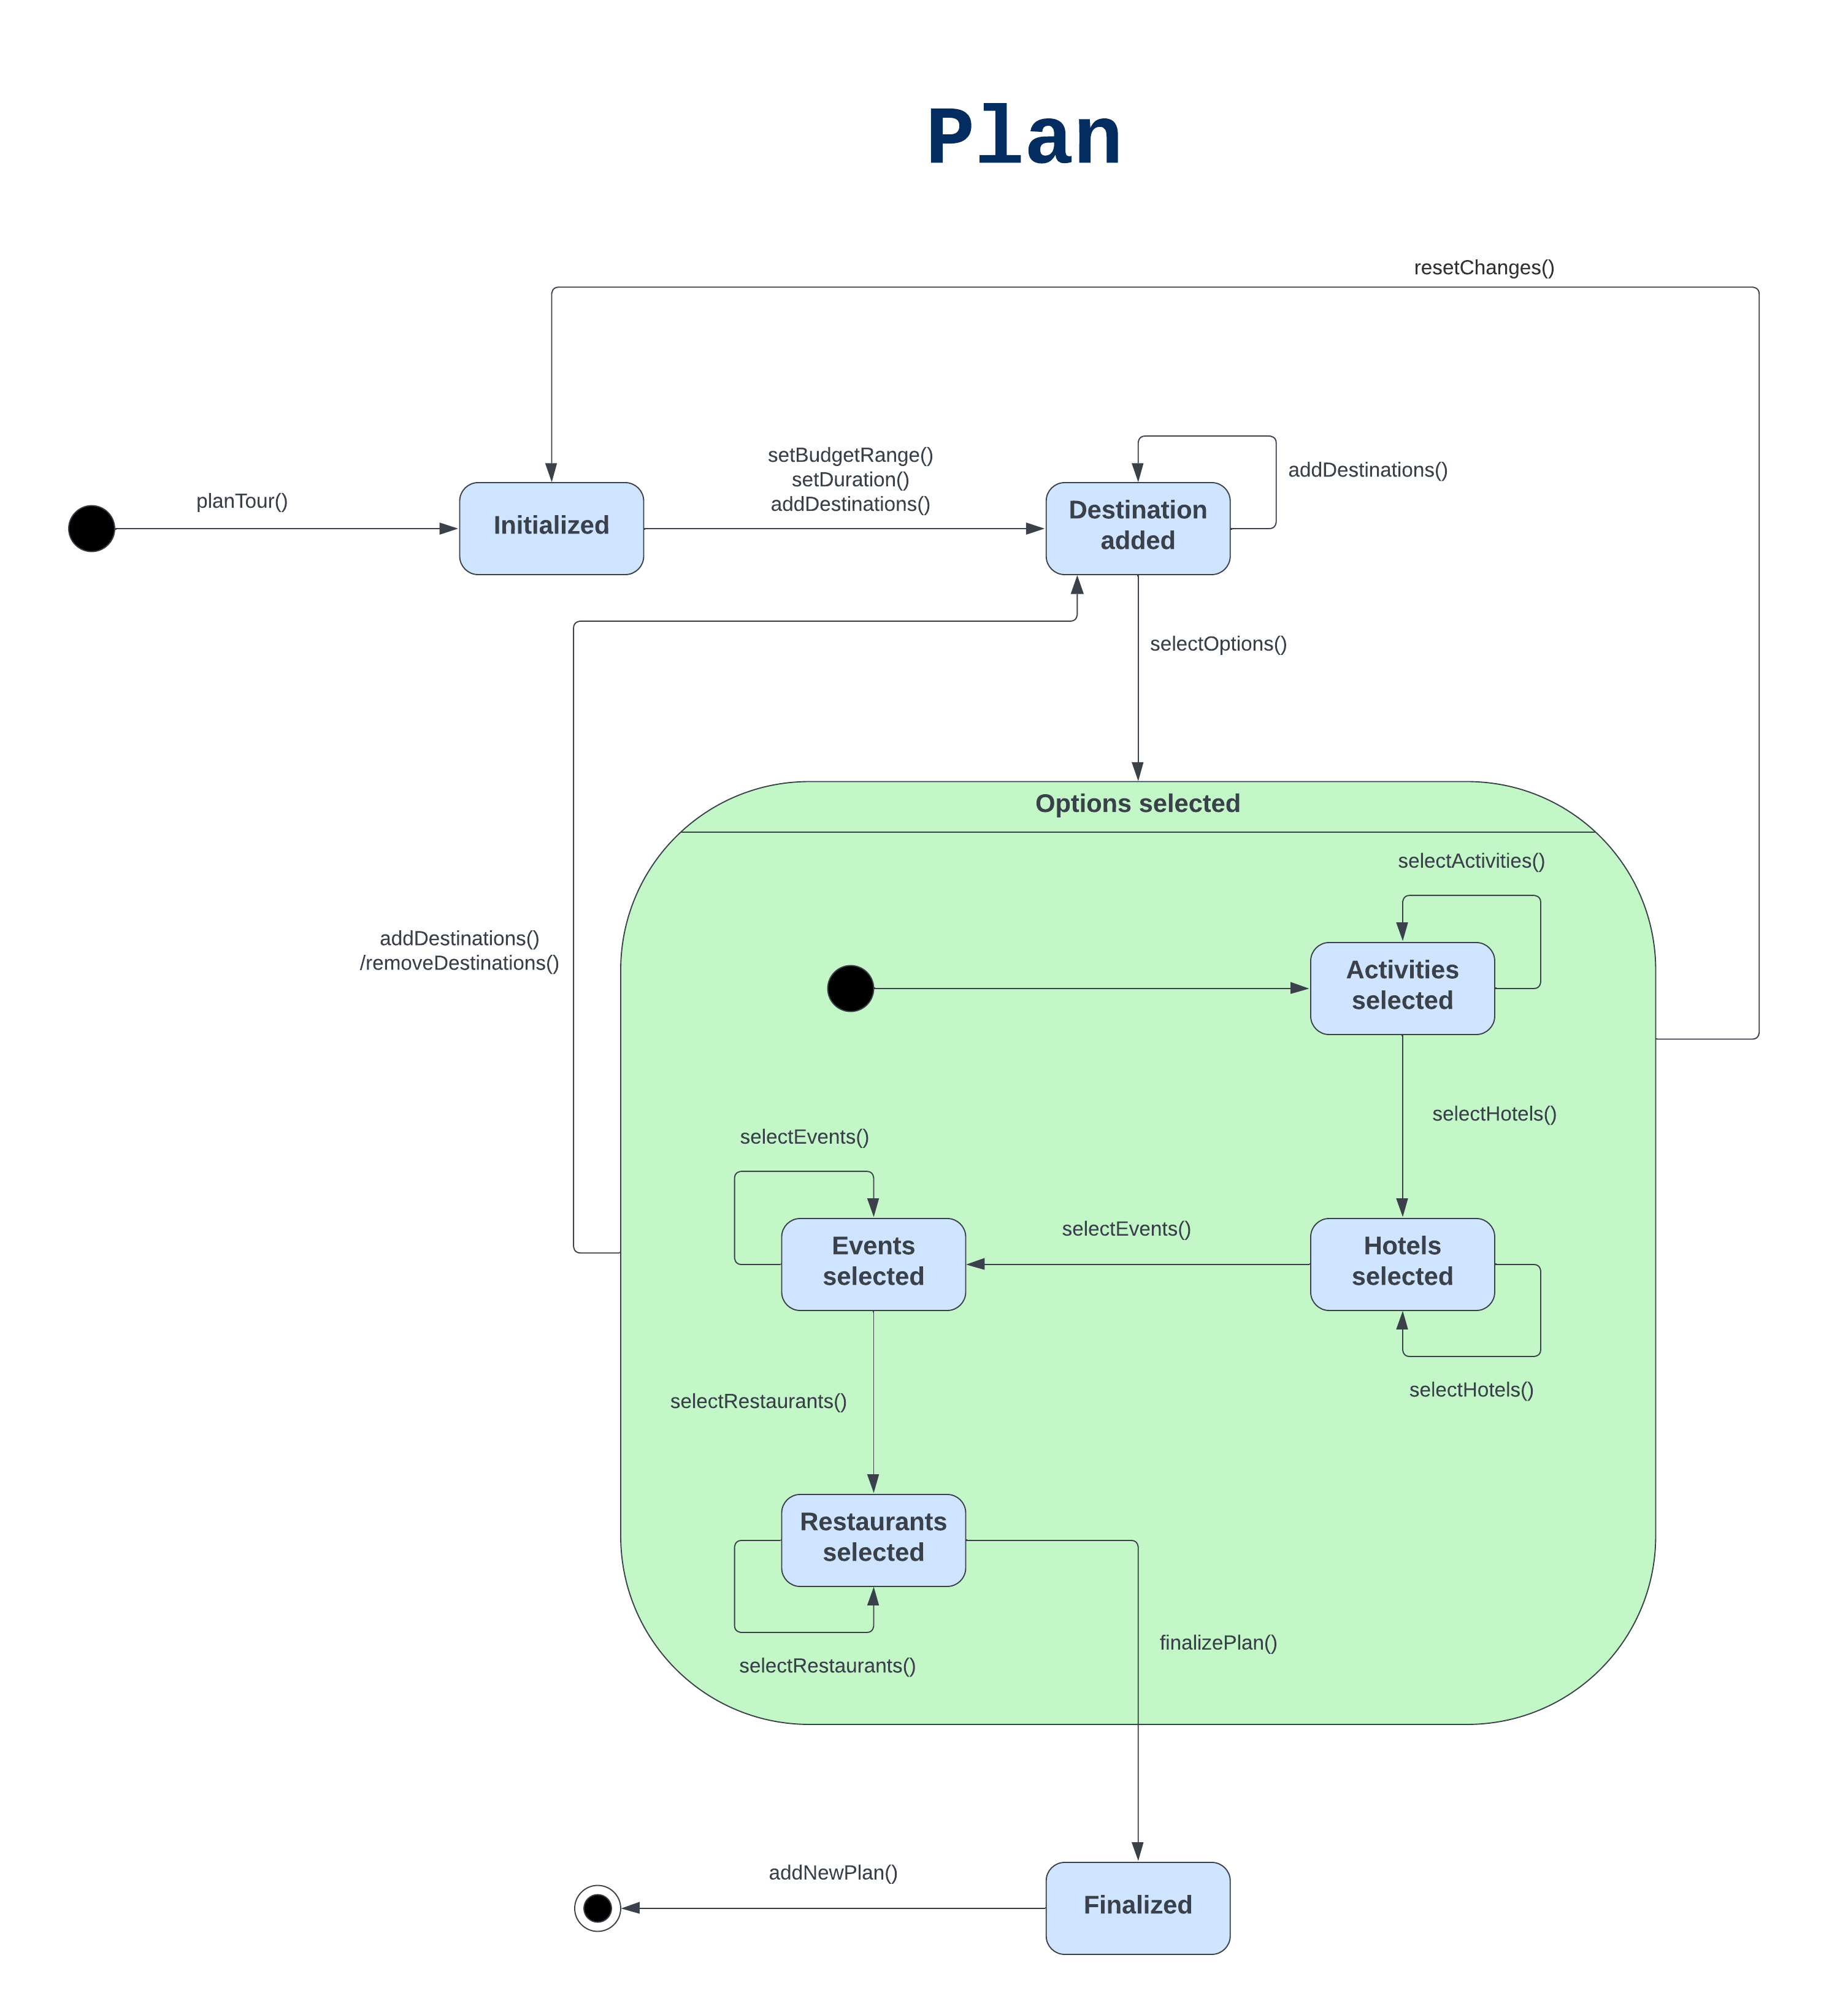
\includegraphics[width=0.85\textwidth]{State Diagram/plan2.png}
        \label{fig:StatePlan}
    \caption{State Diagram for Plan Class}
\end{figure}

\newpage
\subsection{State Diagram for \emph{Tour} Class}
\begin{figure}[H]
    \centering
        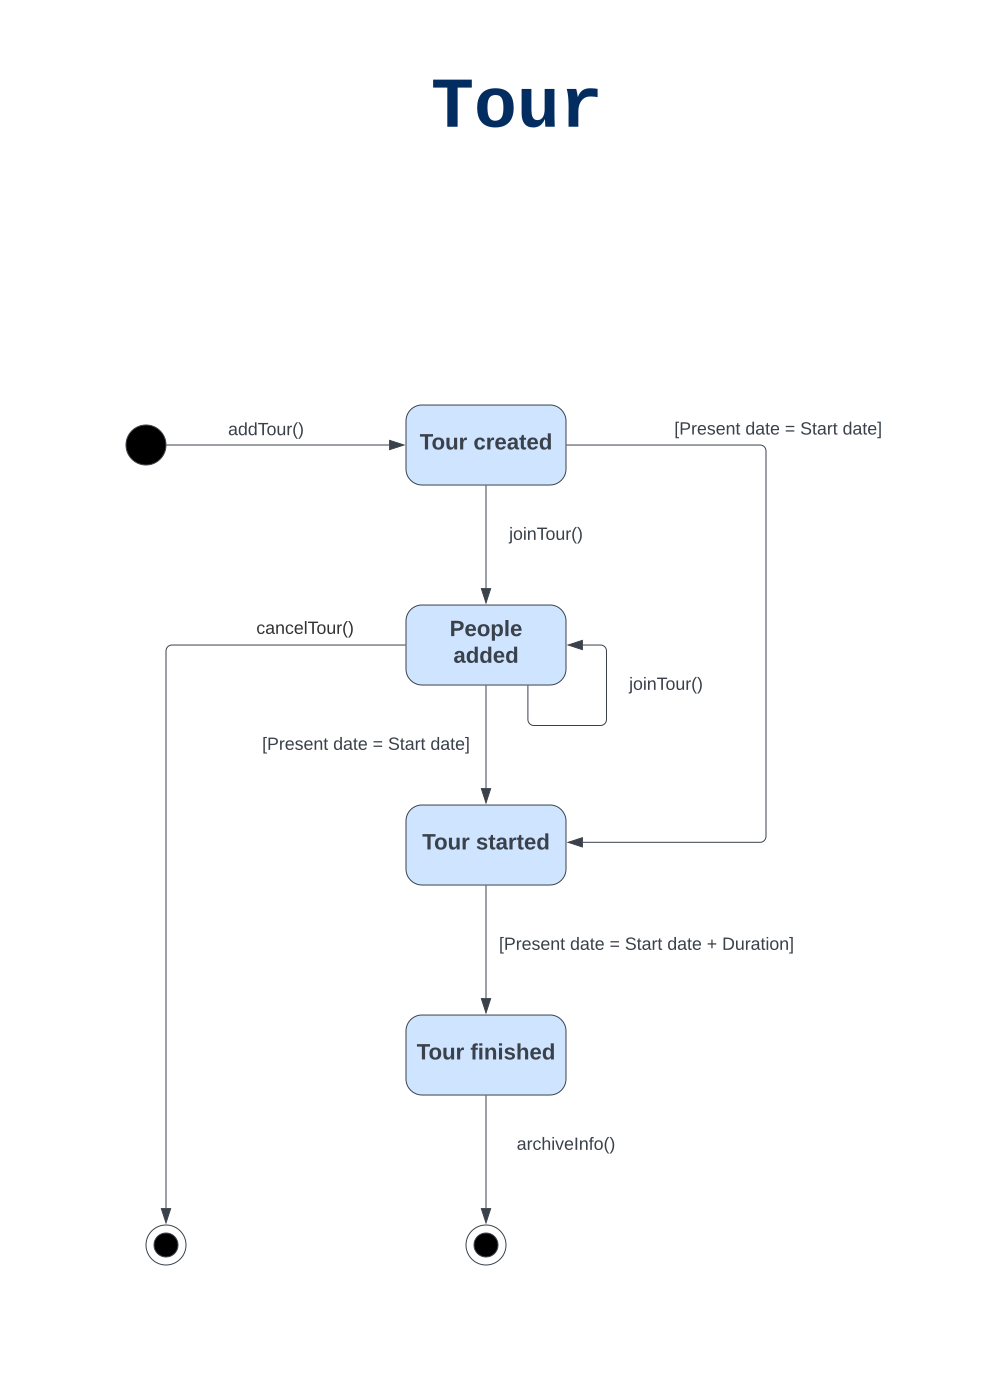
\includegraphics[width=0.85\textwidth]{State Diagram/tour.png}
        \label{fig:StateTour}
    \caption{State Diagram for Tour Class}
\end{figure}

\newpage

\section{Partial Implementation}
\subsection{Implemented Use Case}

\begin{itemize}
    \item Dynamic Plan Generation
\end{itemize}

\subsection{Snippets of the Implemented Pages}
\subsubsection{Home Page}
\begin{figure}[H]
    \centering
        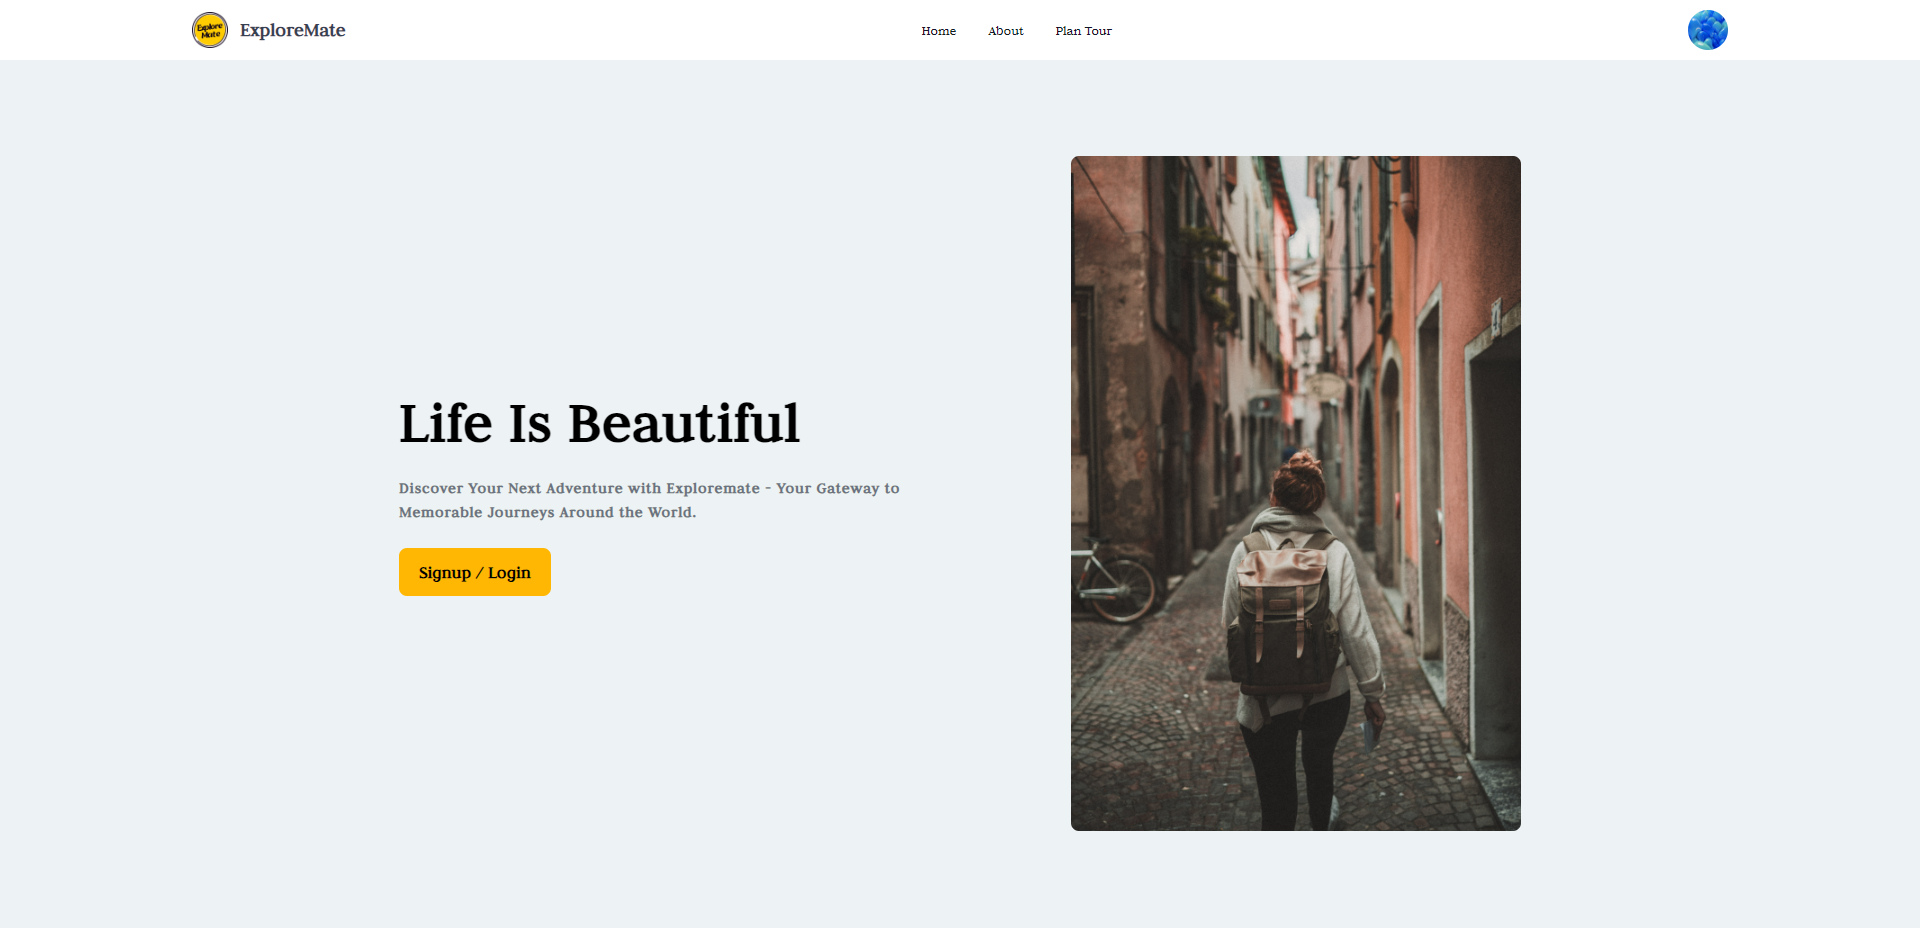
\includegraphics[width=0.85\textwidth]{Frontend SS/Home.png}
        \label{fig:HomePage}
    \caption{Home Page}
\end{figure}

\subsubsection{Plan Initialization}
\begin{figure}[H]
    \centering
        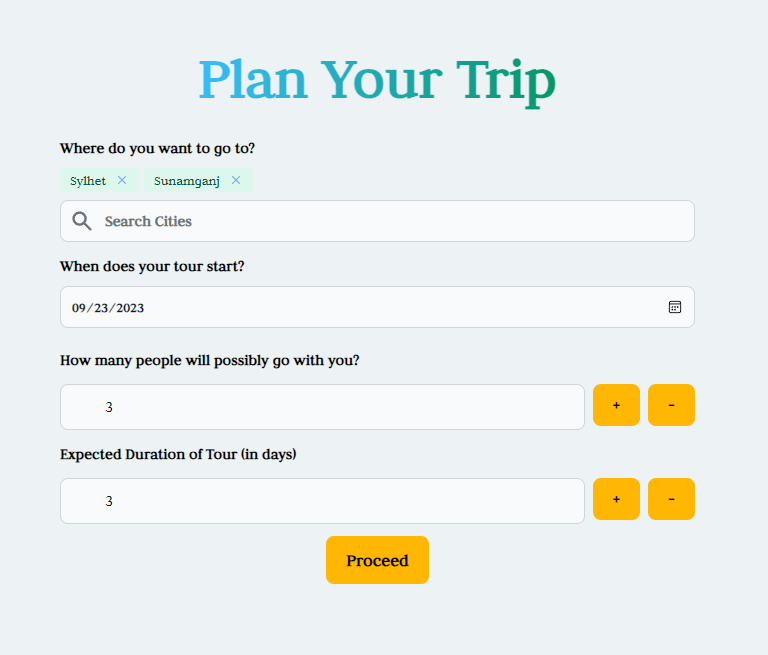
\includegraphics[width=0.60\textwidth]{Frontend SS/Plan Trip.png}
        \label{fig:PlanTrip}
    \caption{Plan Initialization}
\end{figure}

\newpage
\subsubsection{Destination Page}
\begin{figure}[H]
    \centering
        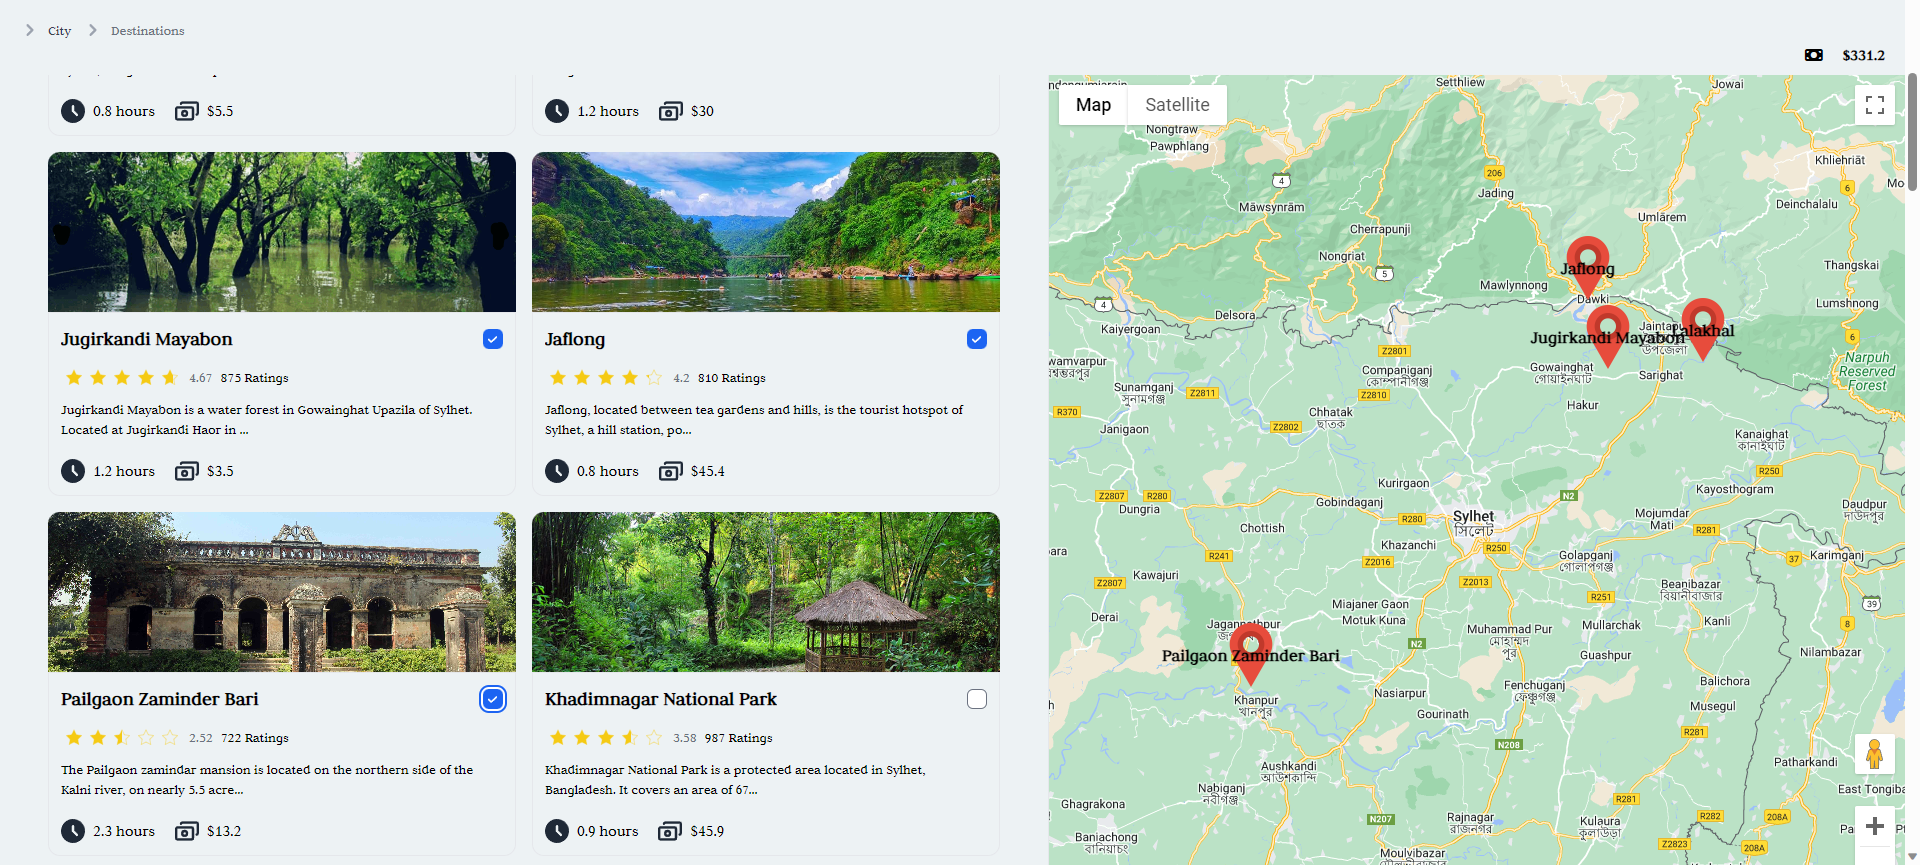
\includegraphics[width=\textwidth]{Frontend SS/Destination1.png}
        \label{fig:Destination1}
    \caption{Destination Page}
\end{figure}
\begin{figure}[H]
    \centering
        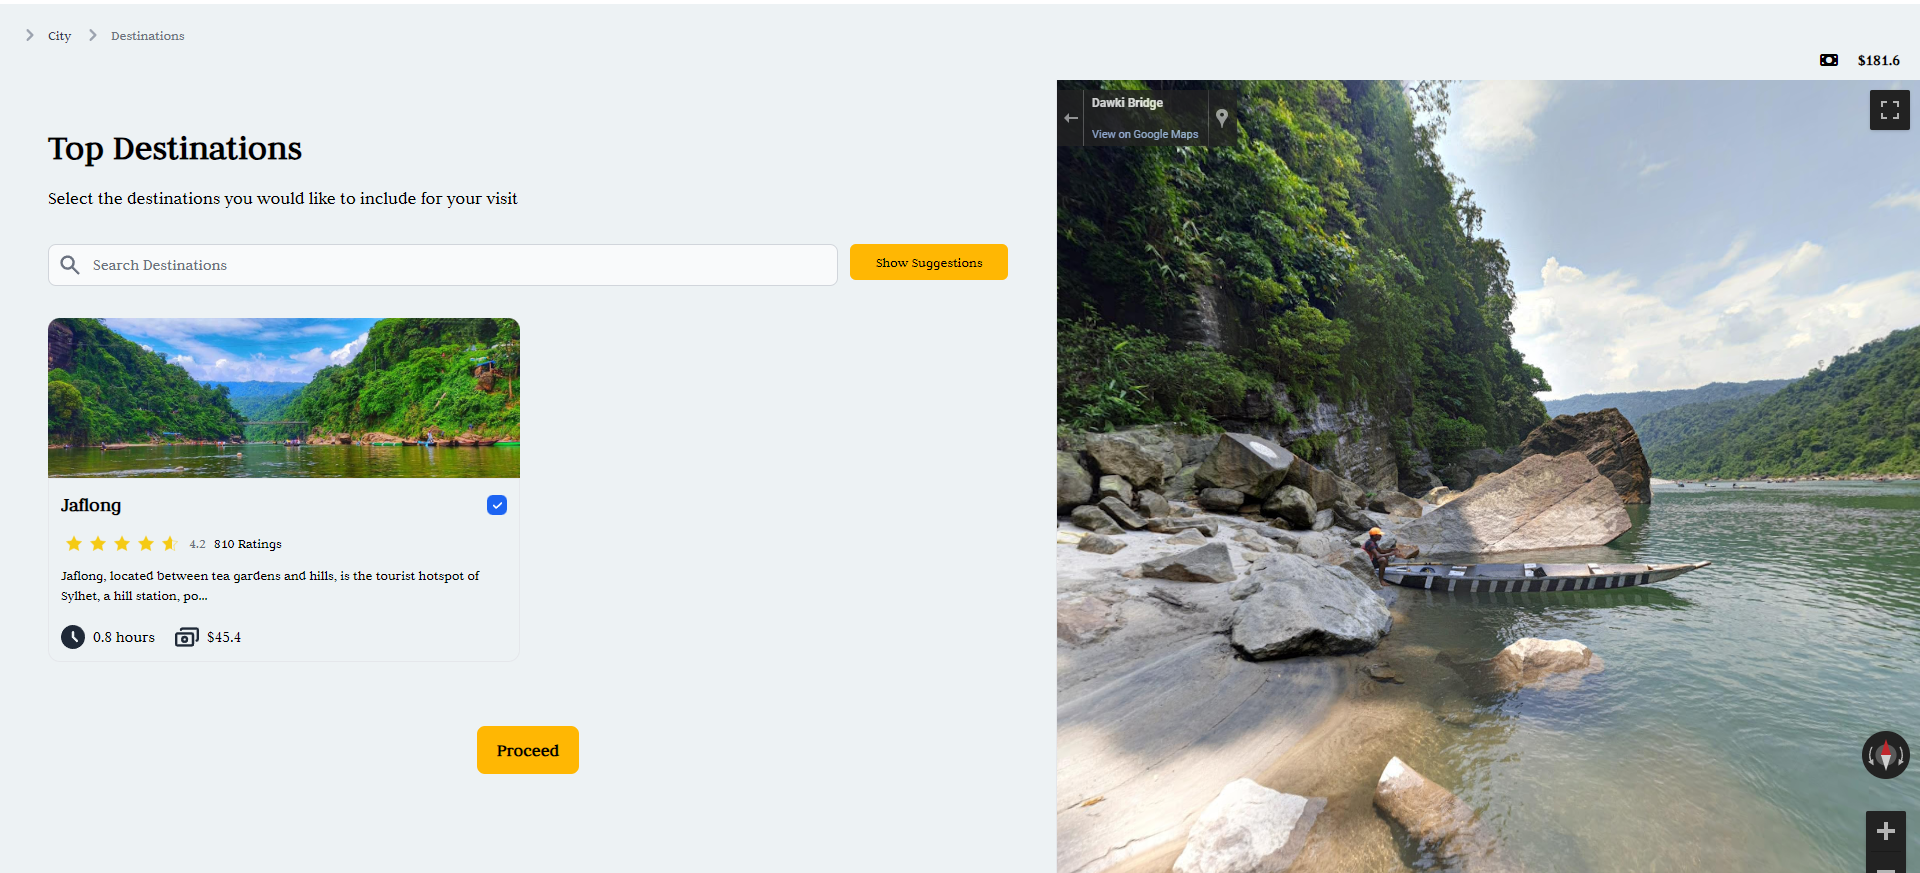
\includegraphics[width=\textwidth]{Frontend SS/Destination Street View.png}
        \label{fig:DestinationStreetView}
    \caption{A Destination with its Street View}
\end{figure}

\subsubsection{Food Page}
\begin{figure}[H]
    \centering
        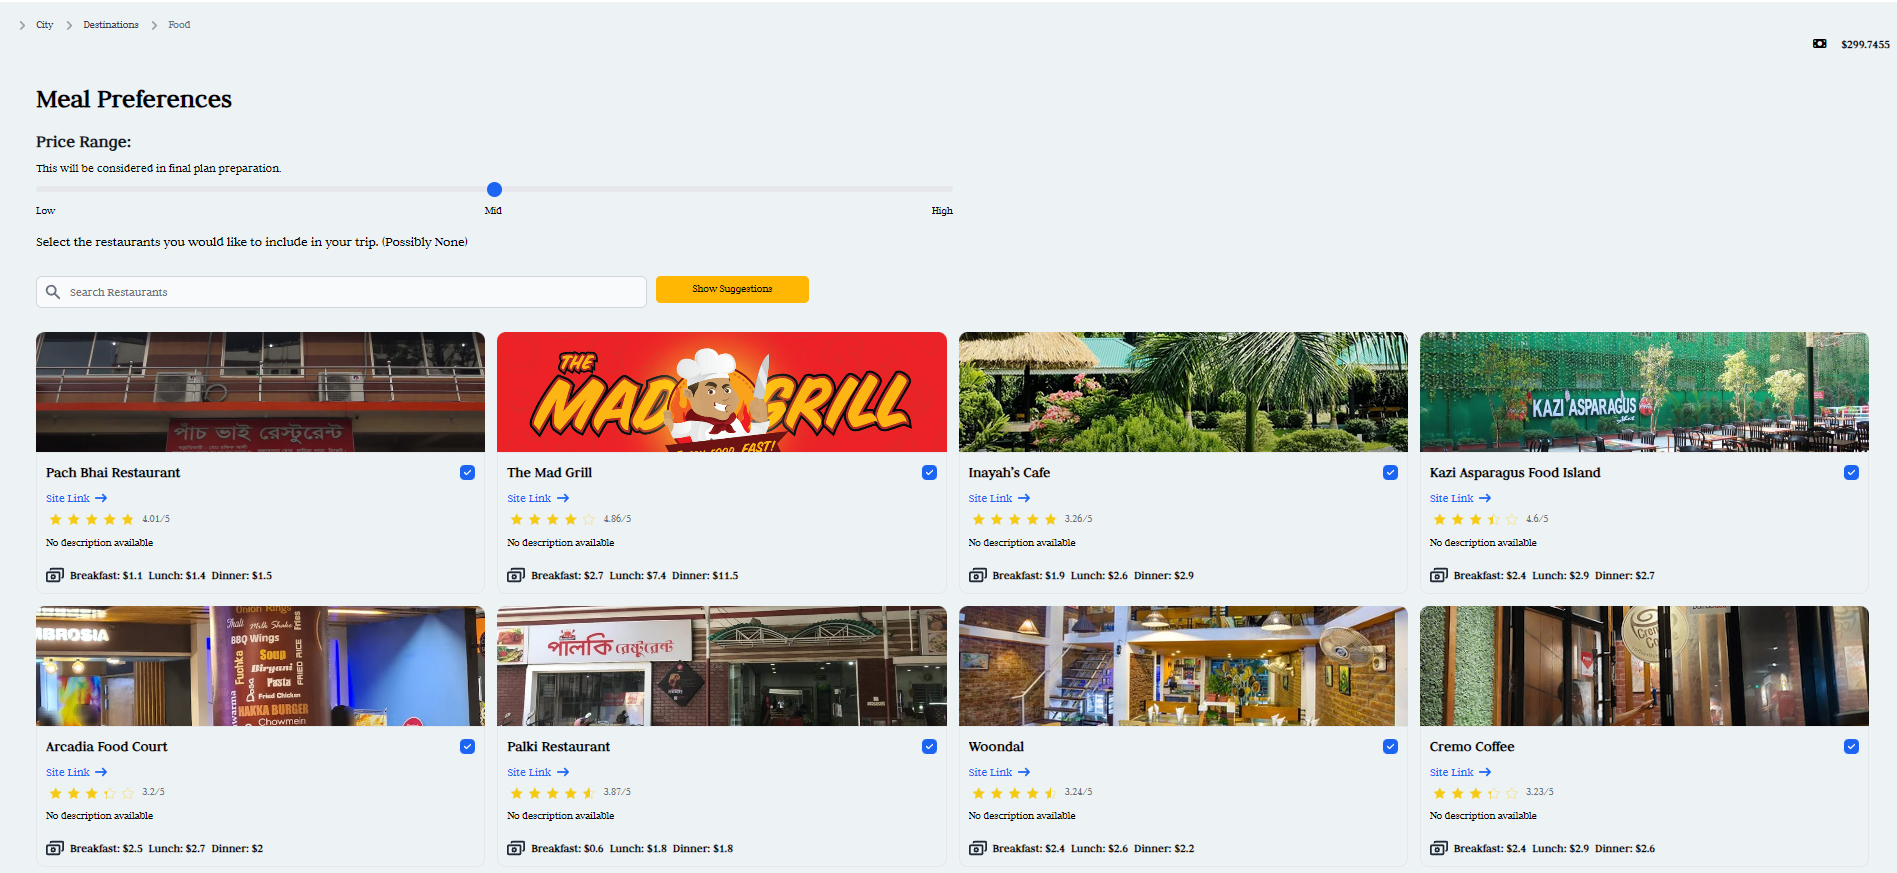
\includegraphics[width=\textwidth]{Frontend SS/Restaurant.png}
        \label{fig:Restaurant}
    \caption{Food Page}
\end{figure}

\subsubsection{Accommodation Page}
\begin{figure}[H]
    \centering
        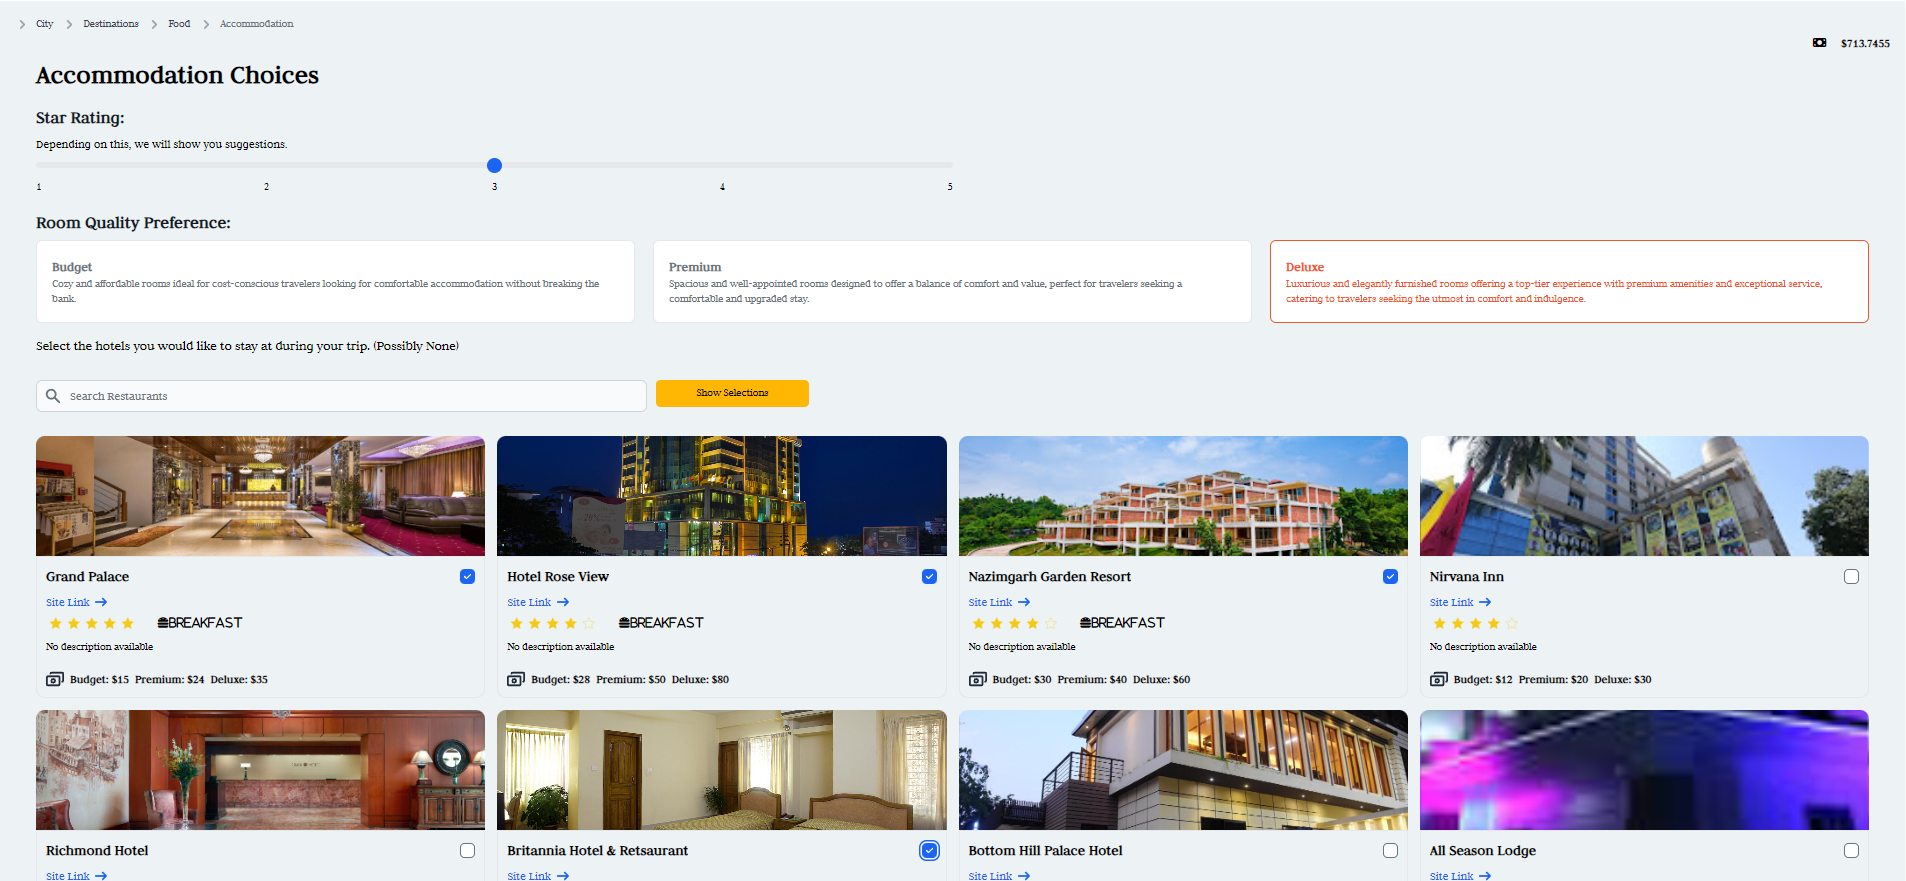
\includegraphics[width=\textwidth]{Frontend SS/Hotel.png}
        \label{fig:Hotel}
    \caption{Accommodation Page}
\end{figure}

\newpage
\subsubsection{Event and Activity Page}
\begin{figure}[H]
    \centering
        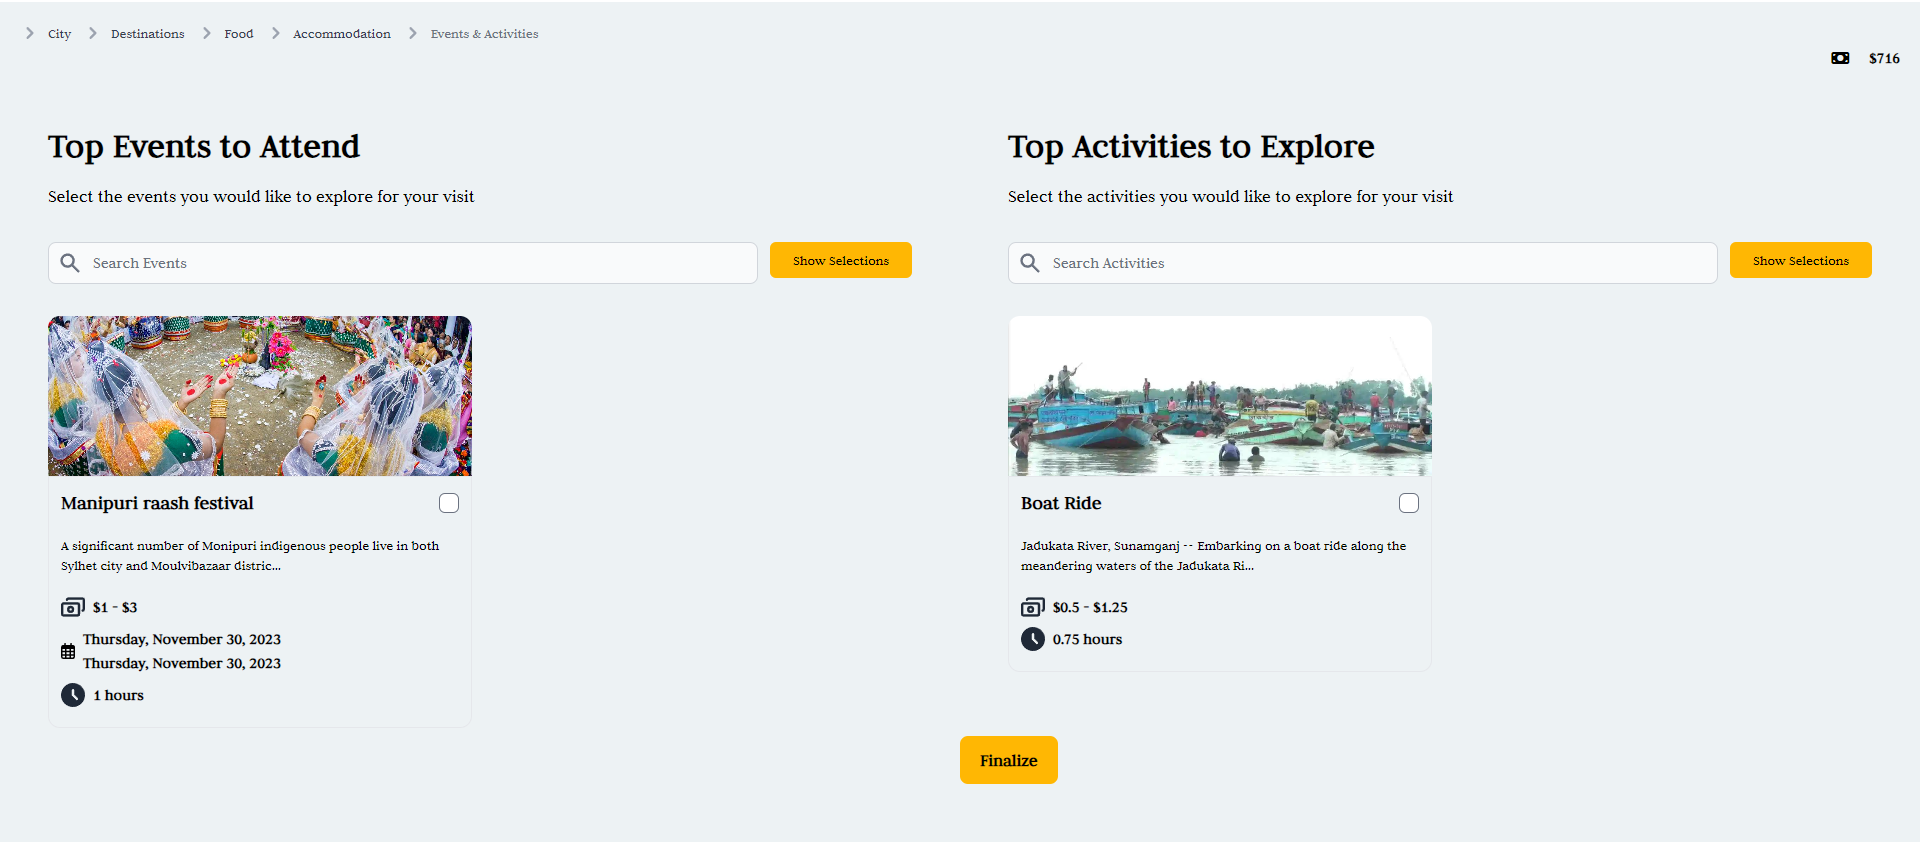
\includegraphics[width=\textwidth]{Frontend SS/Event & Activity.png}
        \label{fig:EventandActivity}
    \caption{Event and Activity Page}
\end{figure}

\subsubsection{Final Plan Page}
\begin{figure}[H]
    \centering
        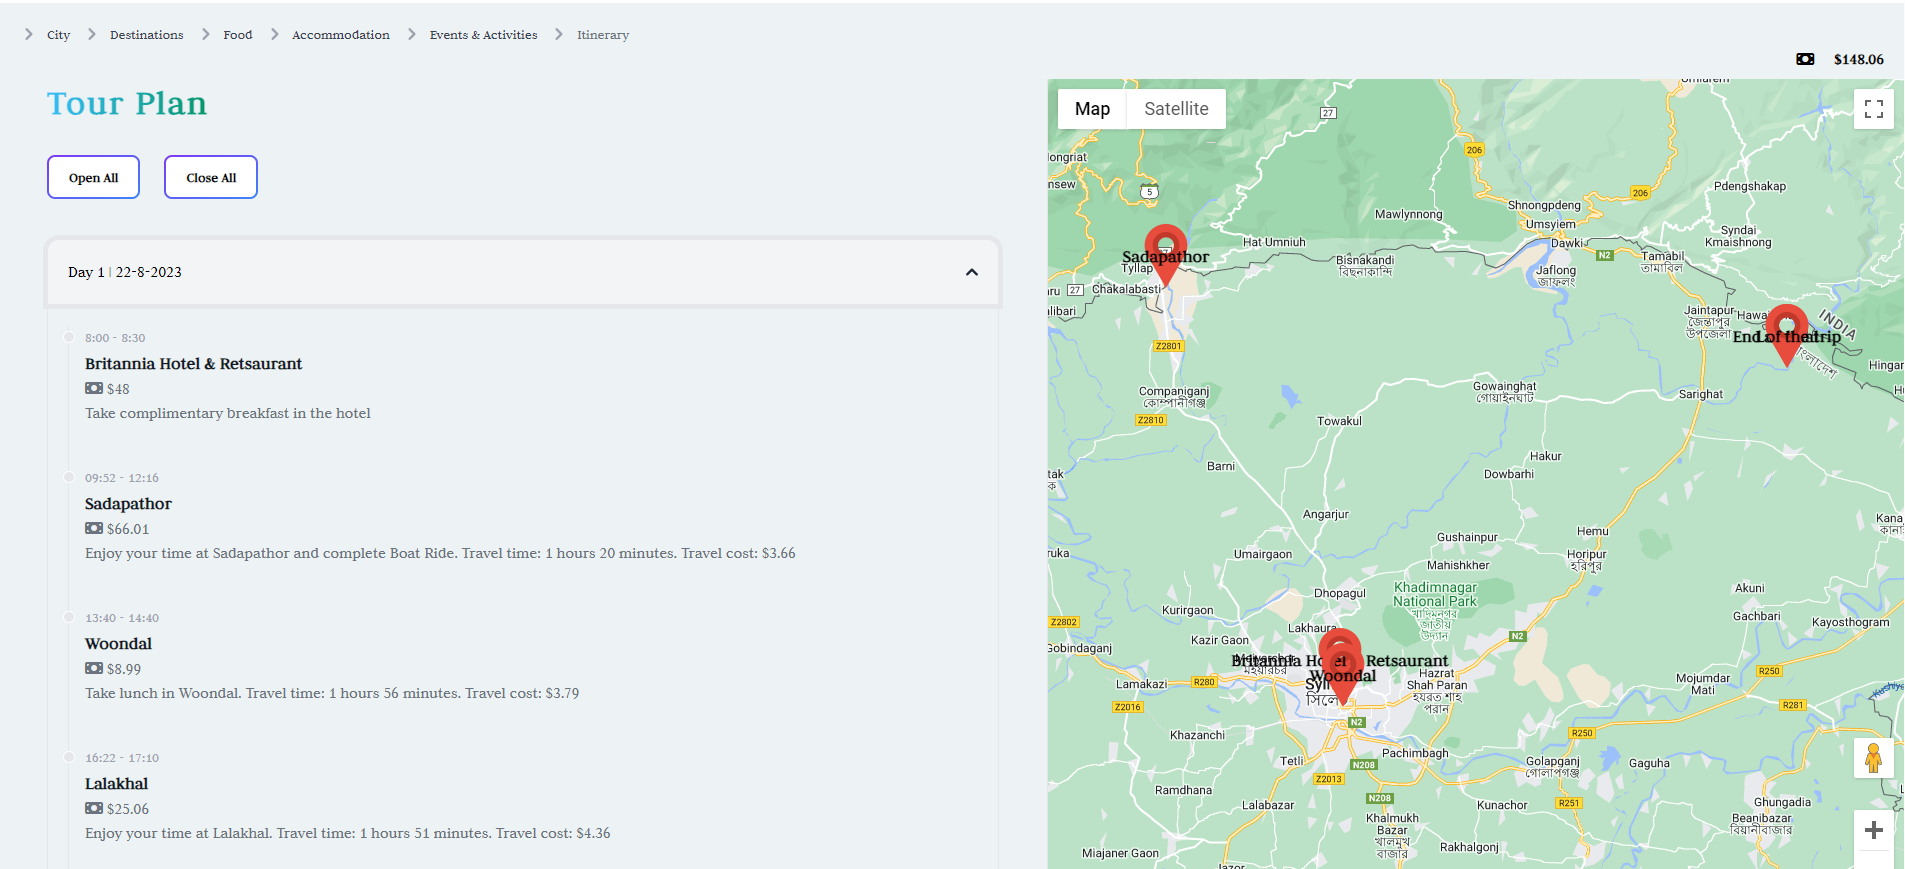
\includegraphics[width=\textwidth]{Frontend SS/Final Plan.png}
        \label{fig:FinalPlan}
    \caption{Final Plan Page}
\end{figure}
\newpage

\subsection{Technology Stack}
\begin{itemize}
    \item \textbf{Database:} PostgreSQL
    \item \textbf{Database Hosting:} SupaBase
    \item \textbf{Backend:} ExpressJS
    \item \textbf{Frontend:} SvelteKit and Tailwind CSS
    \item \textbf{Hosting for Frontend and Backend:} Vercel
    \item \textbf{External APIs:} Google Maps API, Mapbox
\end{itemize}

\subsection{Links}
\begin{itemize}
    \item \href{run: https://exploremate.vercel.app}{Site link}
    \item \href{run: https://github.com/BRAINIAC2677/ExploreMate-Frontend}{Frontend Repository}
    \item \href{run: https://github.com/Sadat-Hossain-01/ExploreMate-Backend}{Backend Repository (Local)}
    \item \href{run: https://github.com/BRAINIAC2677/exploremate-express-api}{Backend Repository (Hosted)}
\end{itemize}

% \subsection{Implemented Algorithm for Plan Generation}
% \begin{enumerate}
%     \item At first, user's selections was taken as input. It includes tour duration, list of selected destinations, hotels, restaurants, events and activities.
%     \item At first a hotel is chosen in the city (If user selects a hotel, it will be chosen, otherwise chosen according to users star preference).
%     \item Then planning from the breakfast is started. If the hotel does not have complimentary breakfast, a restaurant will be chosen (According to users selection or budget preference).
%     \item Then destinations will be selected according to shortest transportation time.
%     \item When it is time for lunch, closest restaurant will be selected for lunch (or users selected restaurant).
%     \item If any destinations are remaining in that city, they will be chosen until dinner time. Otherwise user will start for the second city.
%     \item Plan for next days and next cities will be done in similar fashion until every destination is visited.
    
% \end{enumerate}

\subsection{Feedbacks for Future Modifications}
\begin{itemize}
    \item Giving alternative options for users to choose on different decision points
    \item Adding scope for personalized plans (e.g. according to user's age, medical condition etc.)
\end{itemize}

\end{document}
